\documentclass{beamer}
\usepackage{verbatim}
\usepackage[english]{babel}
\usepackage{multirow}
\usepackage{graphicx}
\setbeamertemplate{caption}[numbered]
\usepackage{subcaption}
\usepackage{xcolor}
\title{Frame Field Generation and Singularity Graph Building}
%\subtitle{Sample Subtitle}

%\usetheme{lucid}

%\graphicspath{{img/}} 

\begin{document}
	\frame {
		\titlepage
	}
	\frame{
		\frametitle{Overall Algorithm Steps}
		\ Given input mesh, 
		\begin{figure}[]
        \center{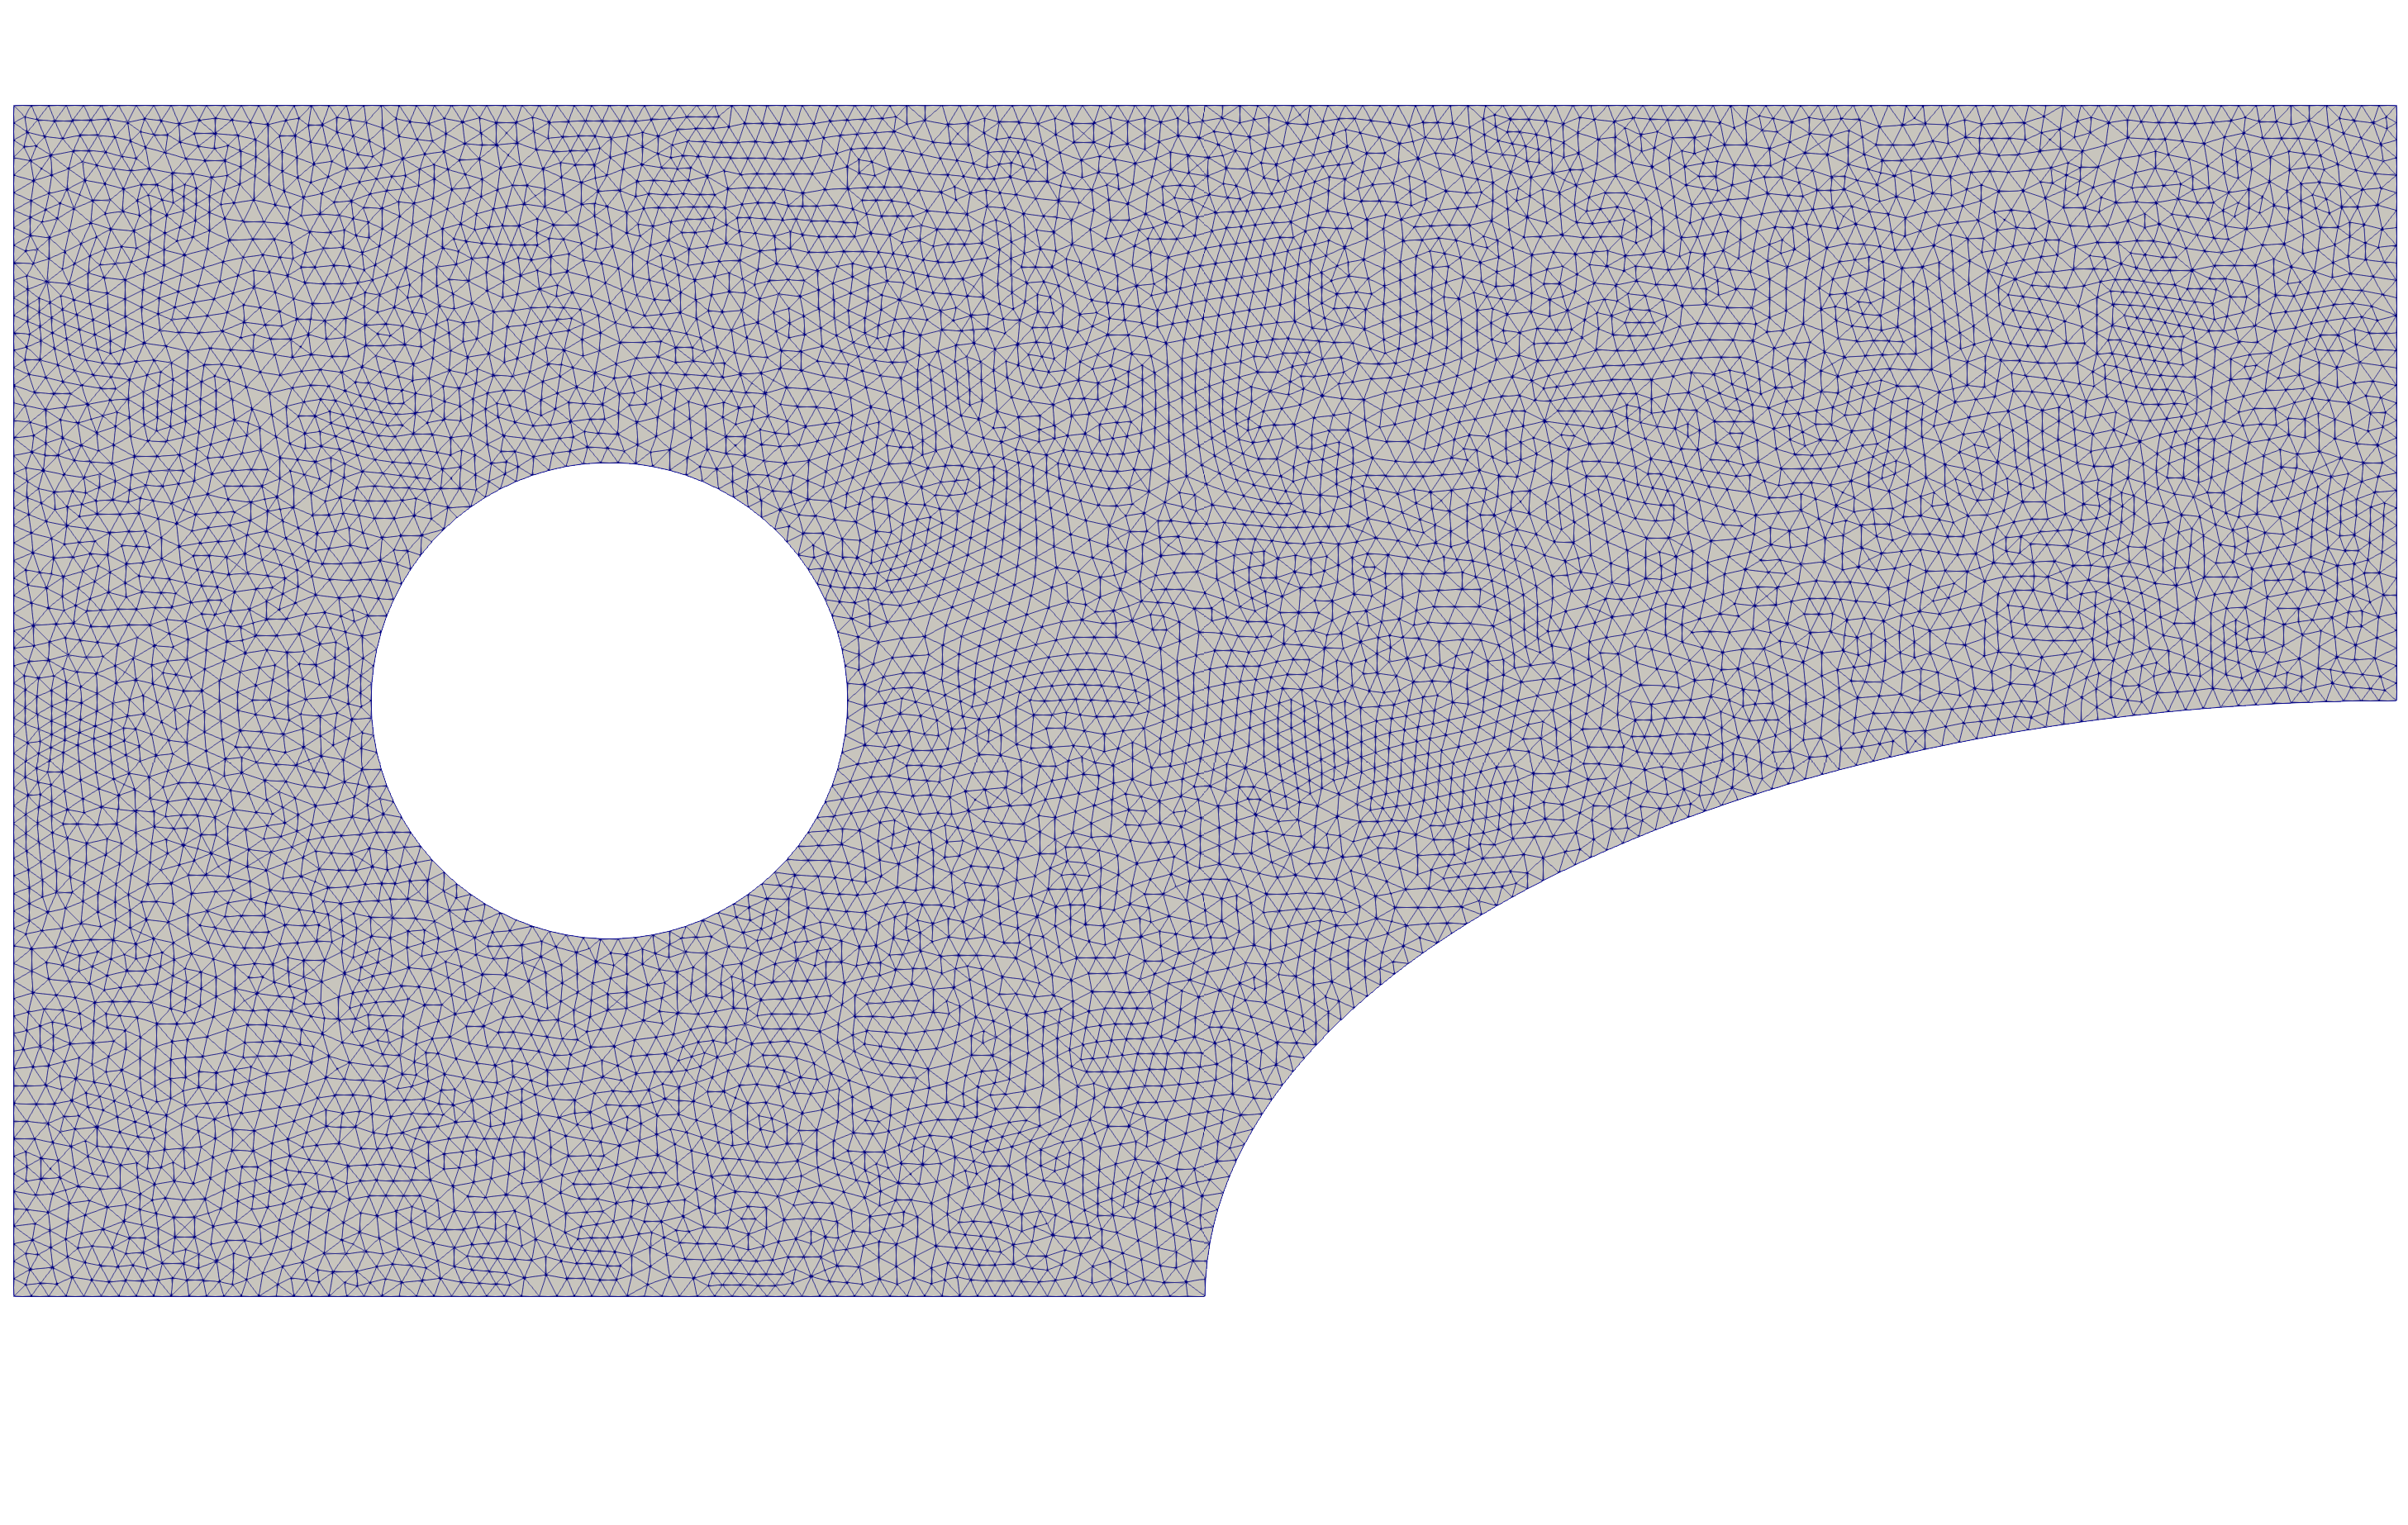
\includegraphics[width=10cm]
        {img/HIS-orig.png}}
        \caption{ Mesh HIS}
      \end{figure}
		 %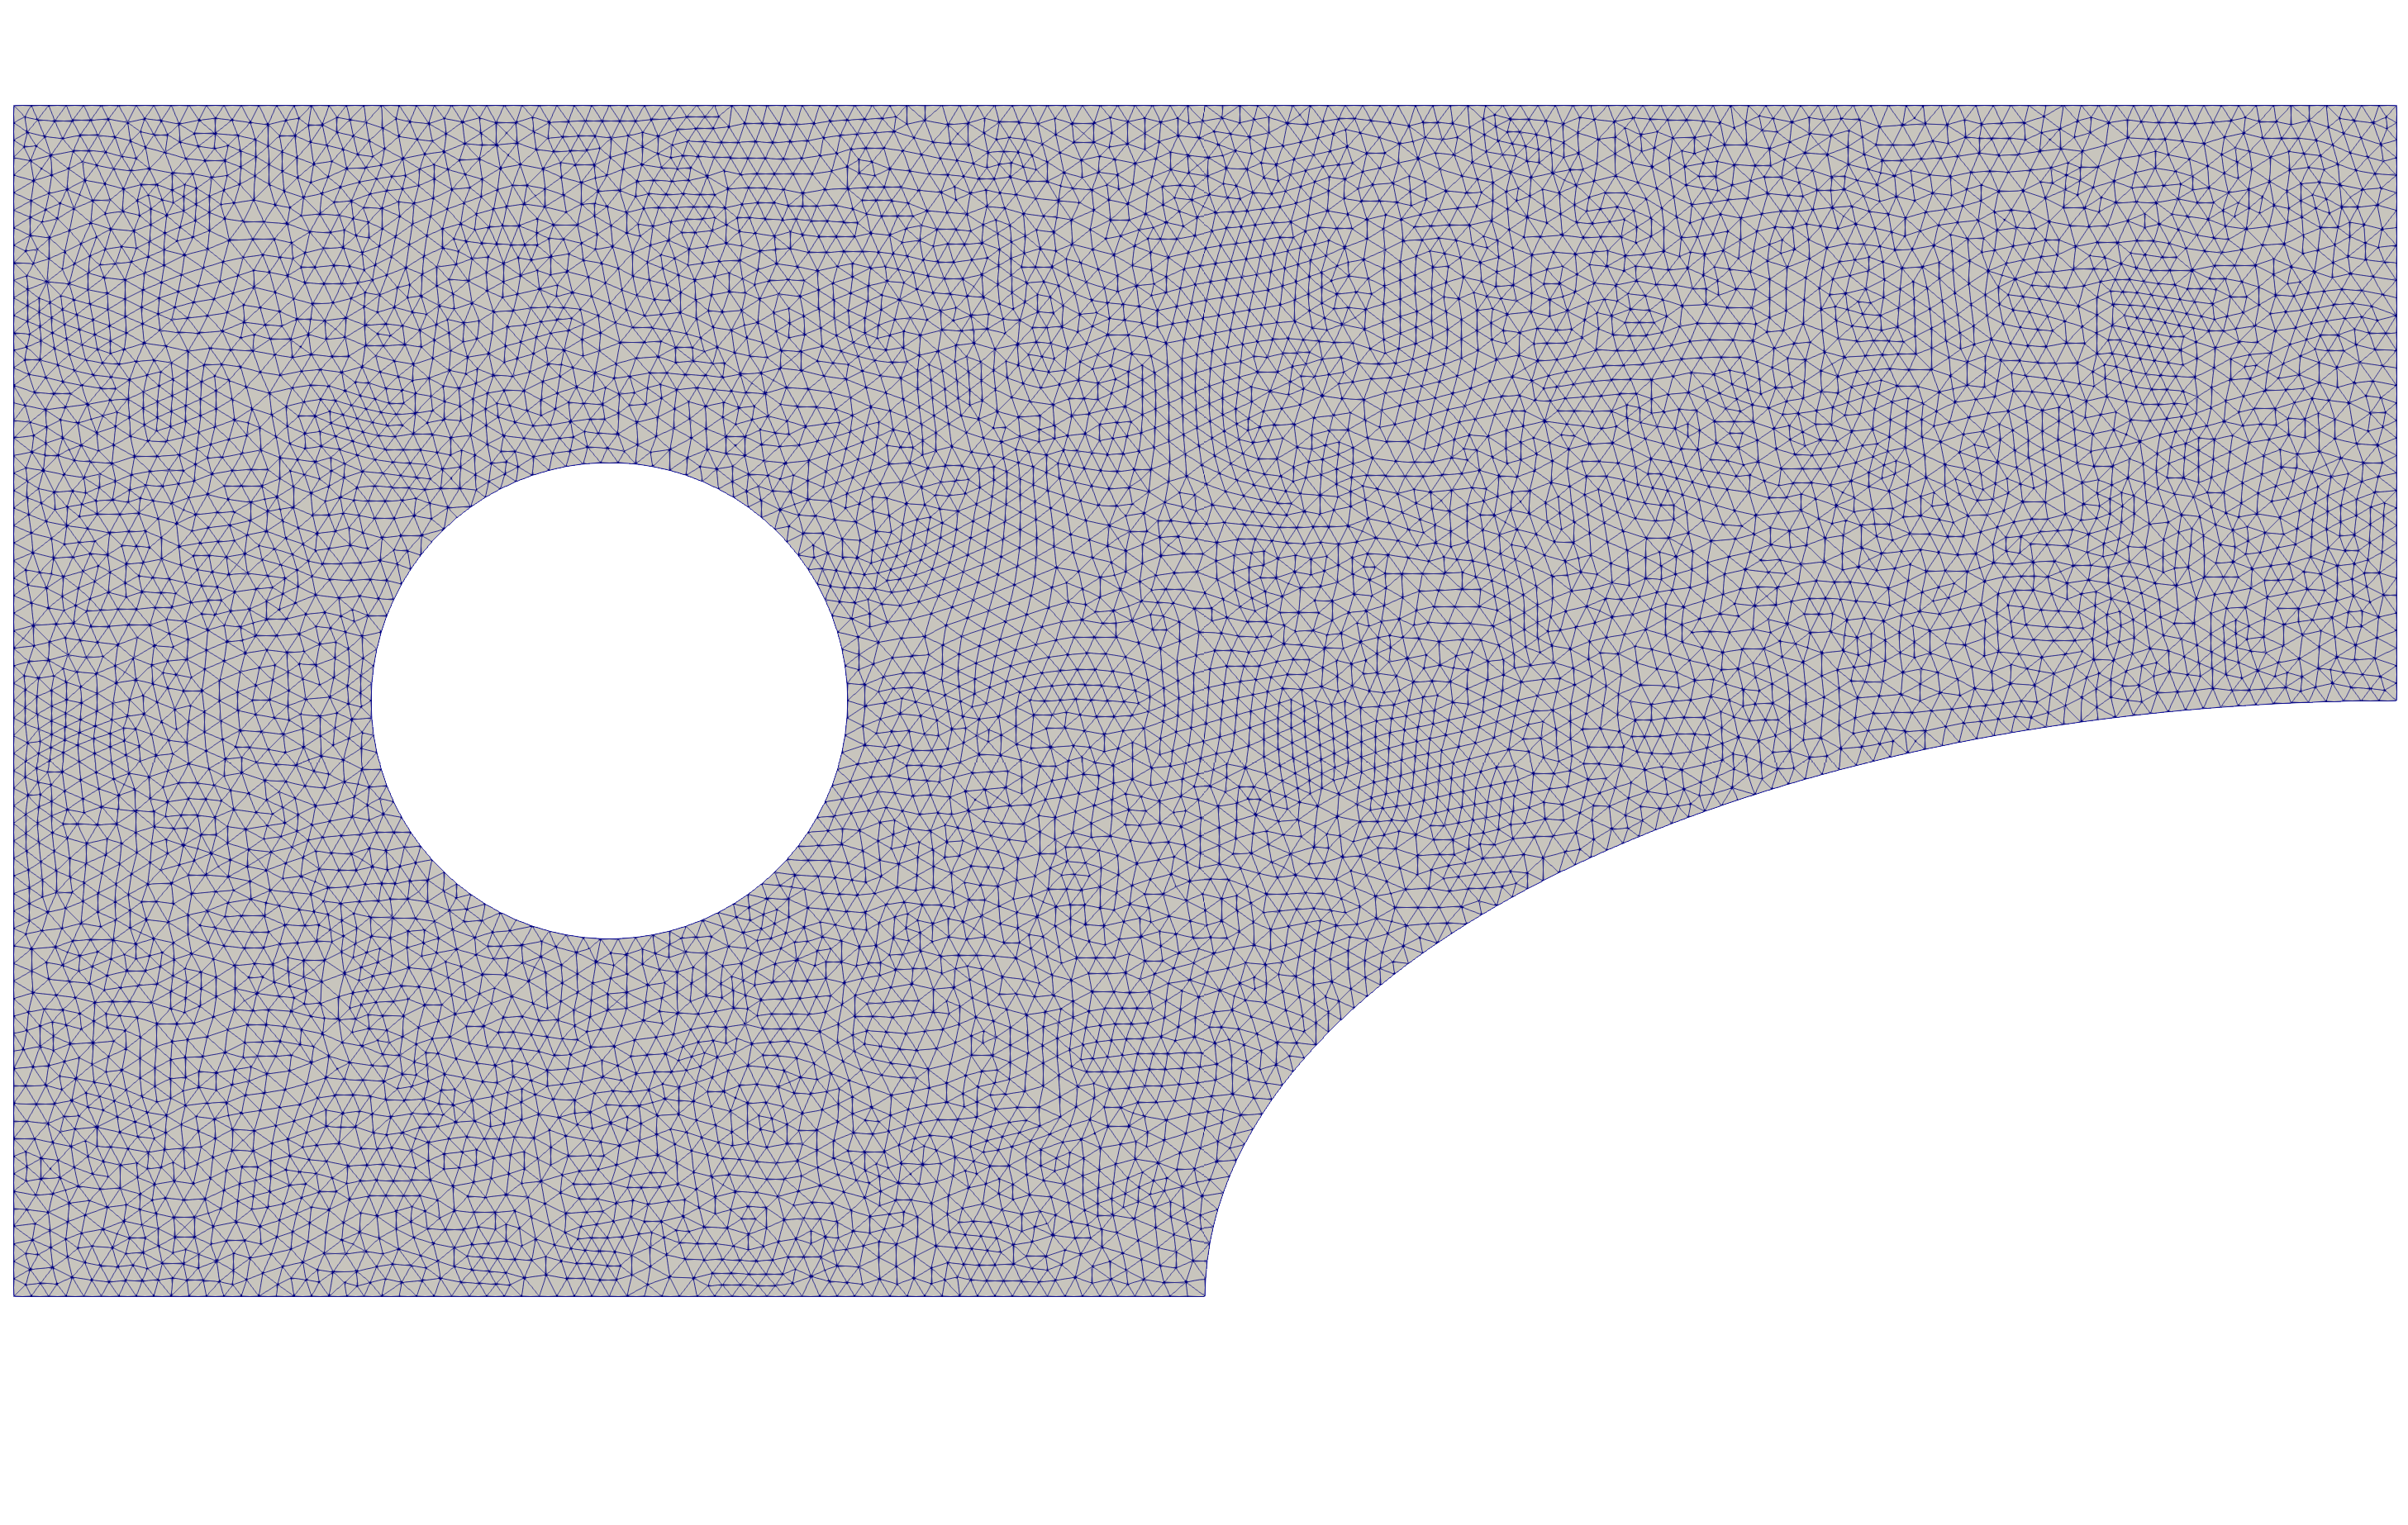
\includegraphics[height=7cm]{img/HIS-orig.png}
	}
	
	%%%%%%%%%%%%%%%%%%%%%%%%%%%%%%%%%%%%%%%%%%%%%%%%%%%%%%%%%%%%%%%%%%%%%%%%%%%%%%%%%%%%%%%%
	\frame{
		\frametitle{Overall Algorithm Steps}		
		\begin{itemize}
			\item 1. Construct Frame Field			
			
		\end{itemize}
		
		\begin{figure}[]
        \center{\includegraphics[width=10cm]
        {img/HIS-frame.png}}
        \caption{ Mesh HIS - Frame Field}
      \end{figure}
		%\includegraphics[height=7cm]{img/HIS-frame.png}
	}
	%%%%%%%%%%%%%%%%%%%%%%%%%%%%%%%%%%%%%%%%%%%%%%%%%%%%%%%%%%%%%%%%%%%%%%%%%%%%%%%%%%%%%%%%
	
	\frame{
		\frametitle{Overall Algorithm Steps}		
		\begin{itemize}
			\item 1. Construct Frame Field			
			
		\end{itemize}
		\begin{figure}[]
        \center{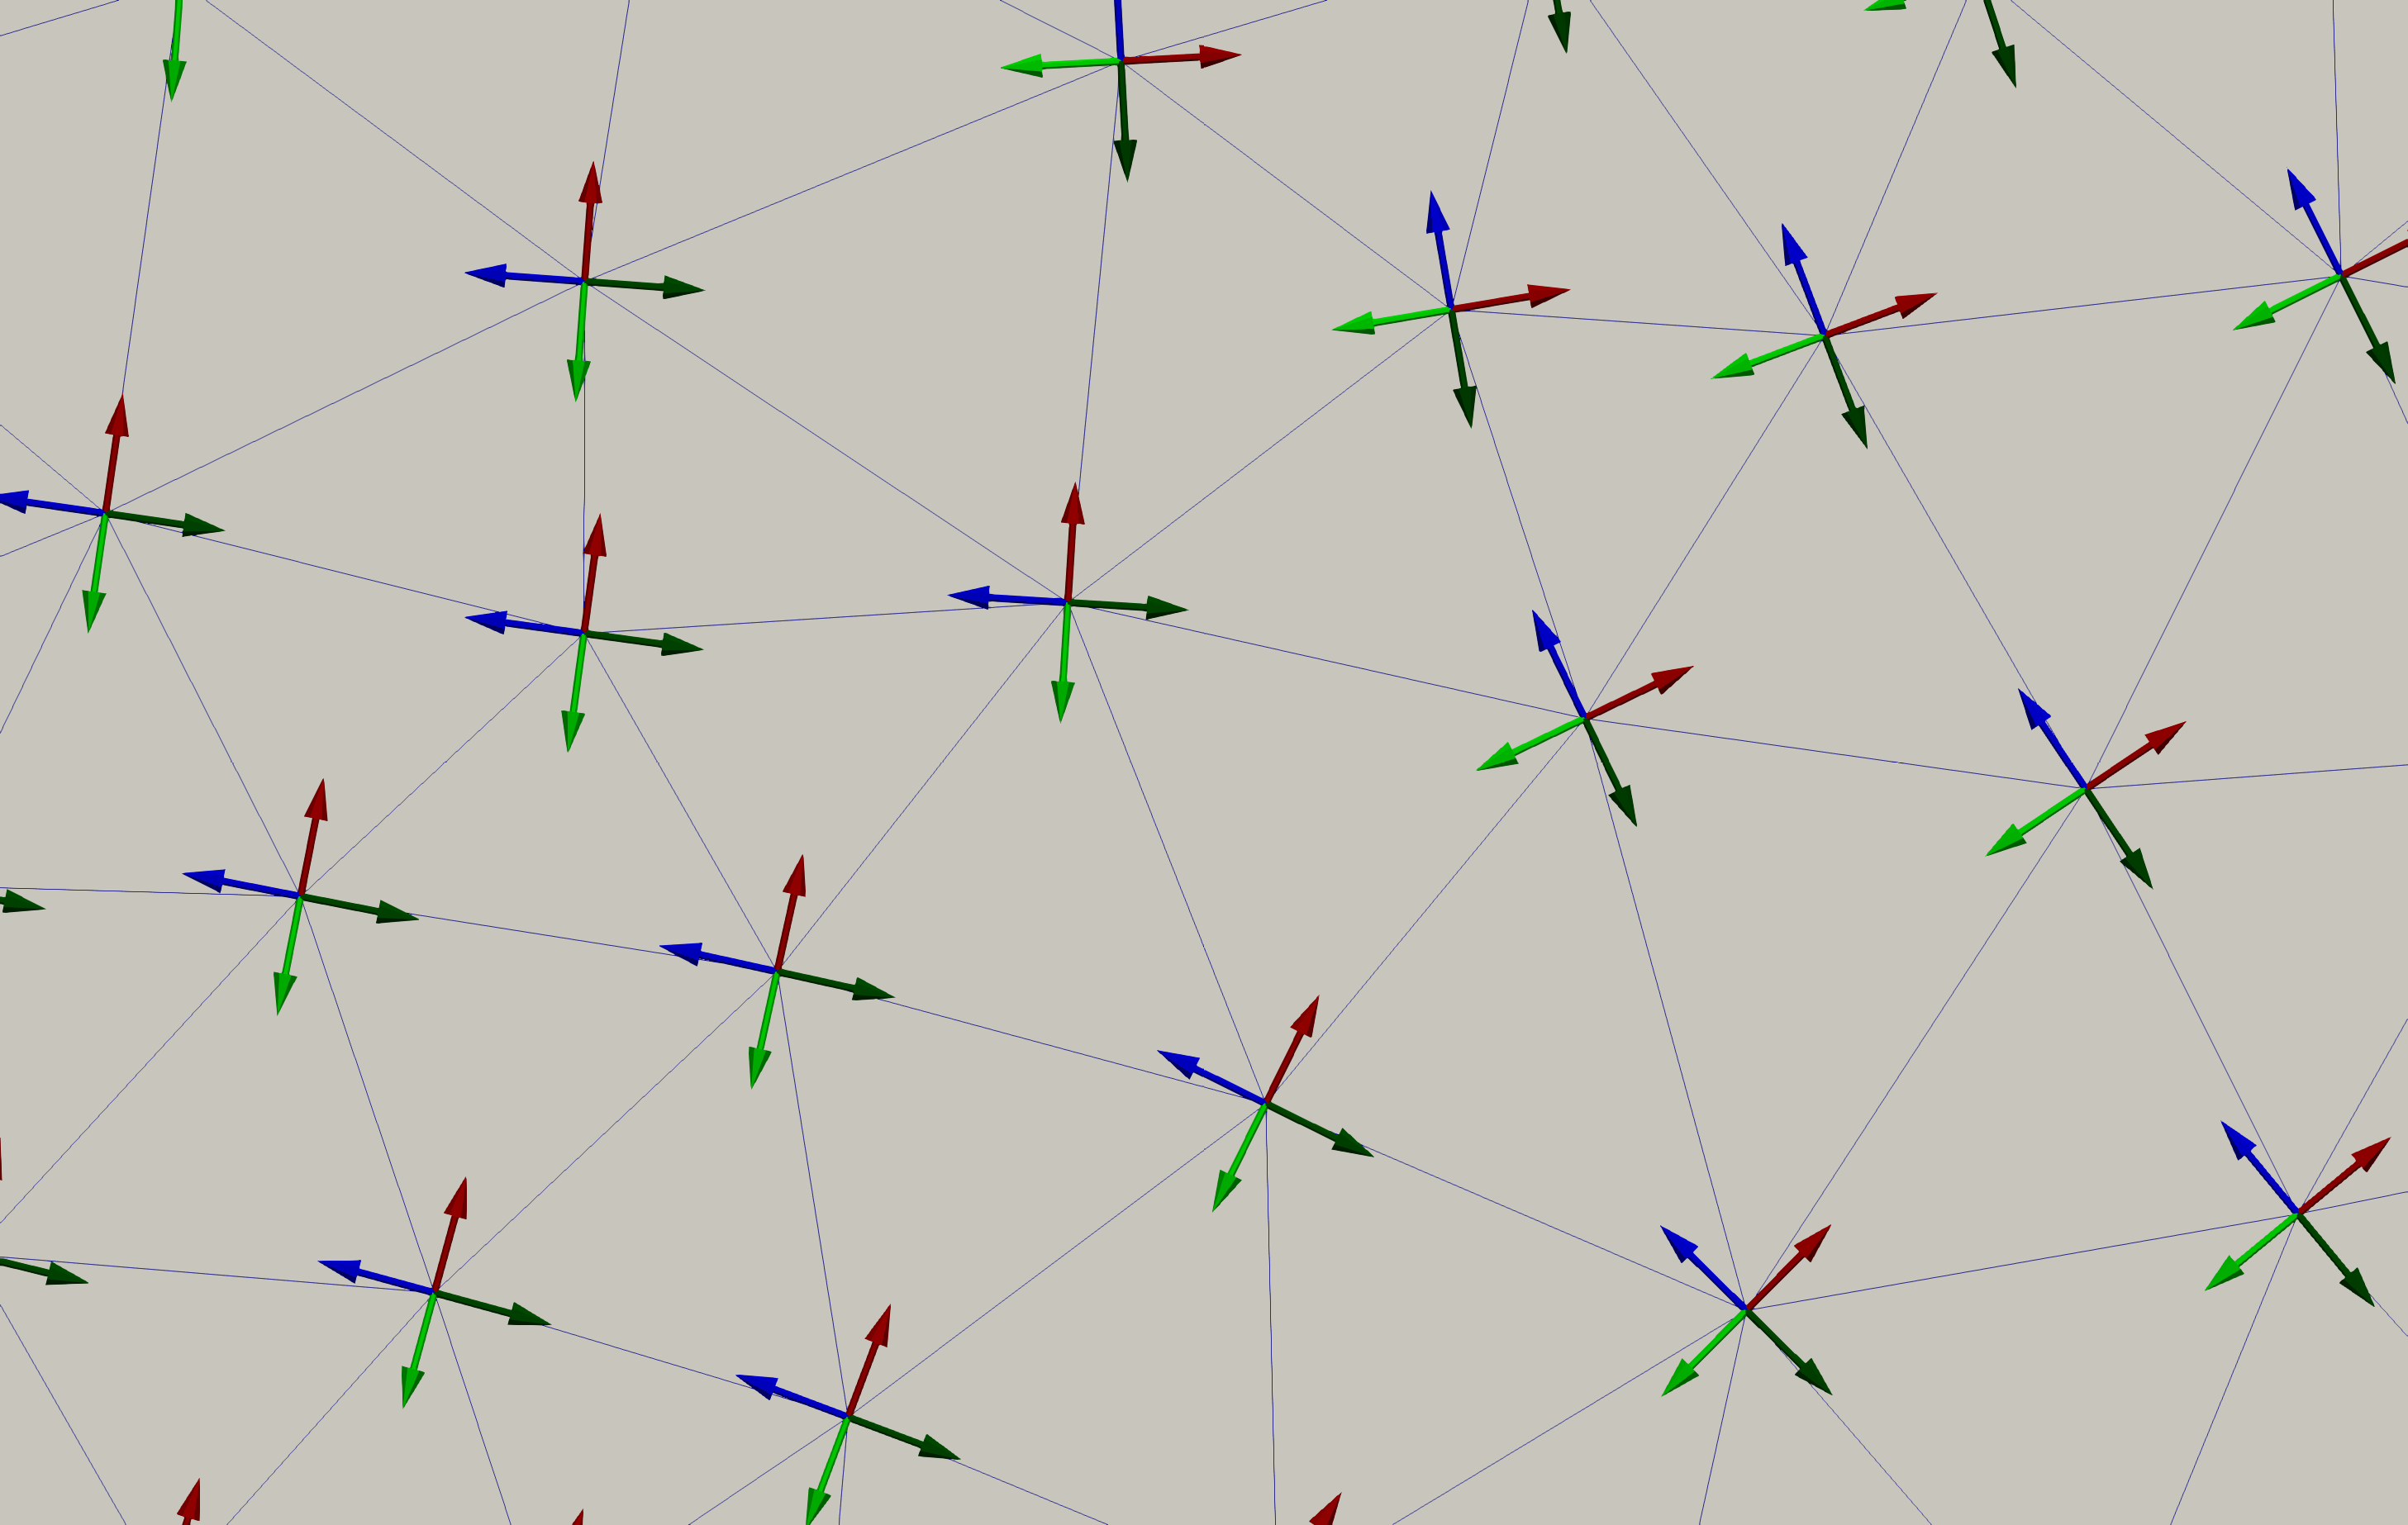
\includegraphics[width=10cm]
        {img/HIS-frame-close-up.png}}
        \caption{ Mesh HIS - Frame Field - close-up}
      \end{figure}
		%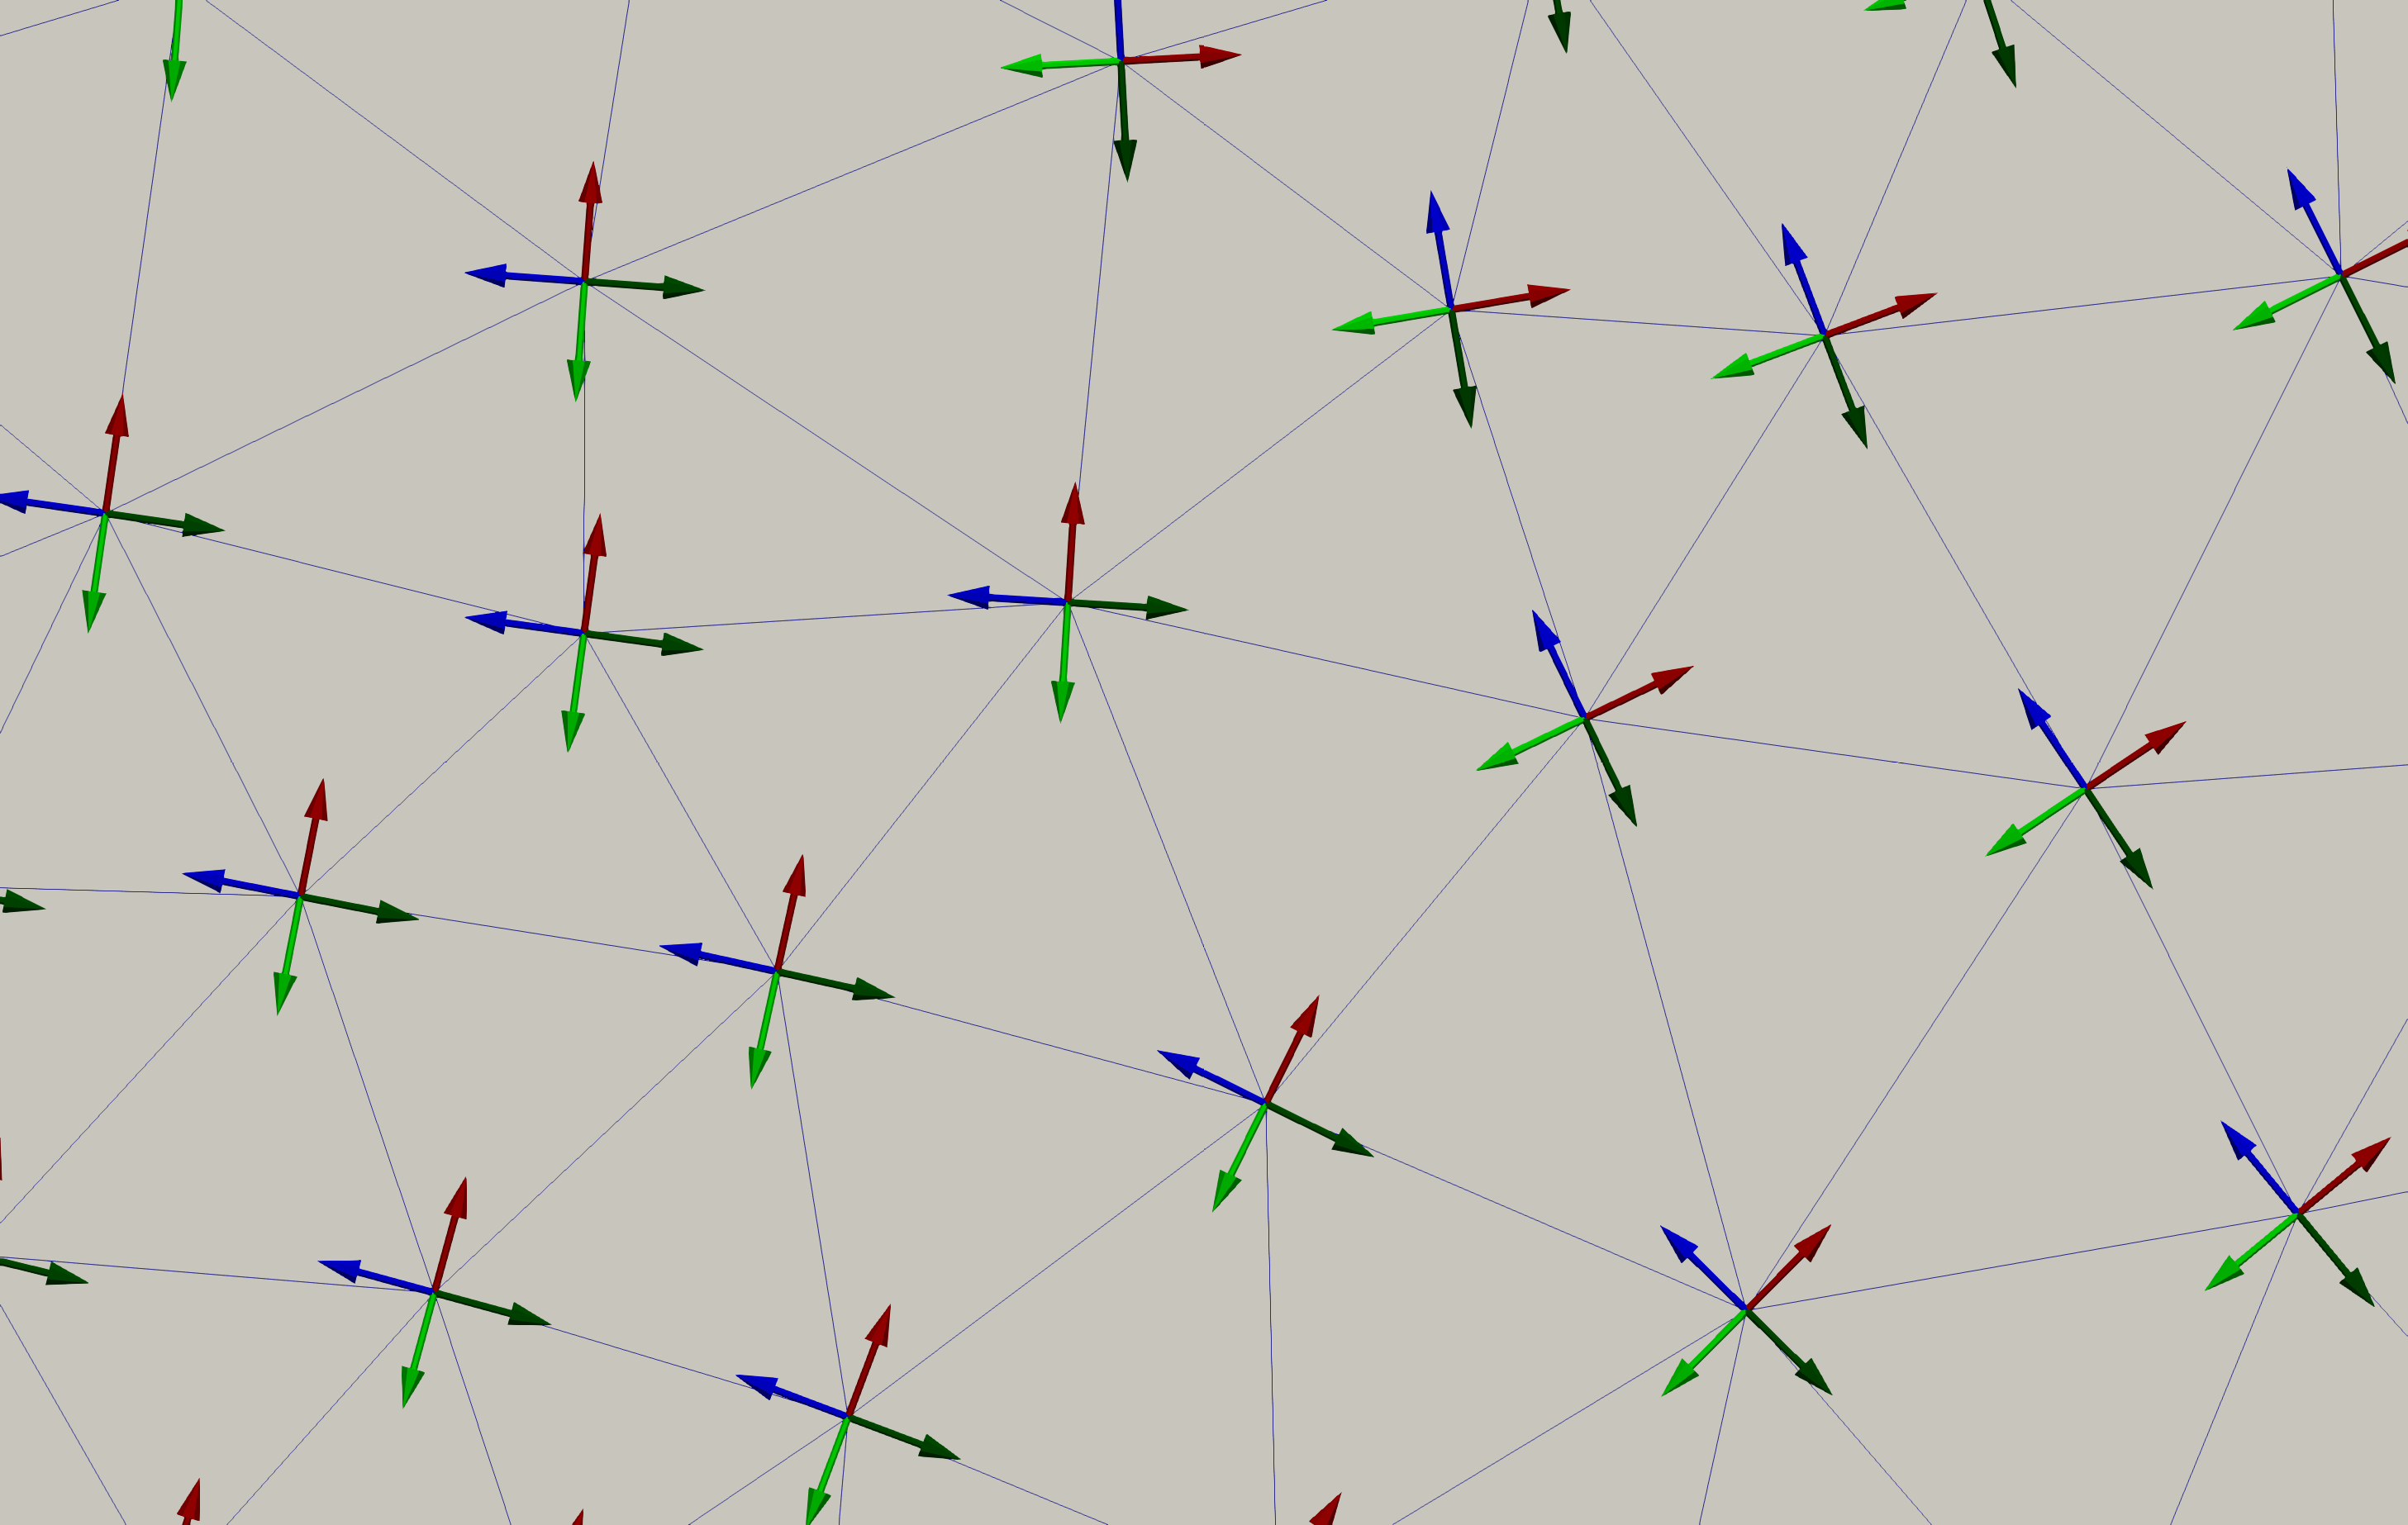
\includegraphics[height=7cm]{img/HIS-frame-close-up.png}
	}
	
	%%%%%%%%%%%%%%%%%%%%%%%%%%%%%%%%%%%%%%%%%%%%%%%%%%%%%%%%%%%%%%%%%%%%%%%%%%%%%%%%%%%%%%%%
	\frame{
		\frametitle{Overall Algorithm Steps}		
		\begin{itemize}				
			\item 2. Construct Singularity Graph
			
		\end{itemize}
		\begin{figure}[]
        \center{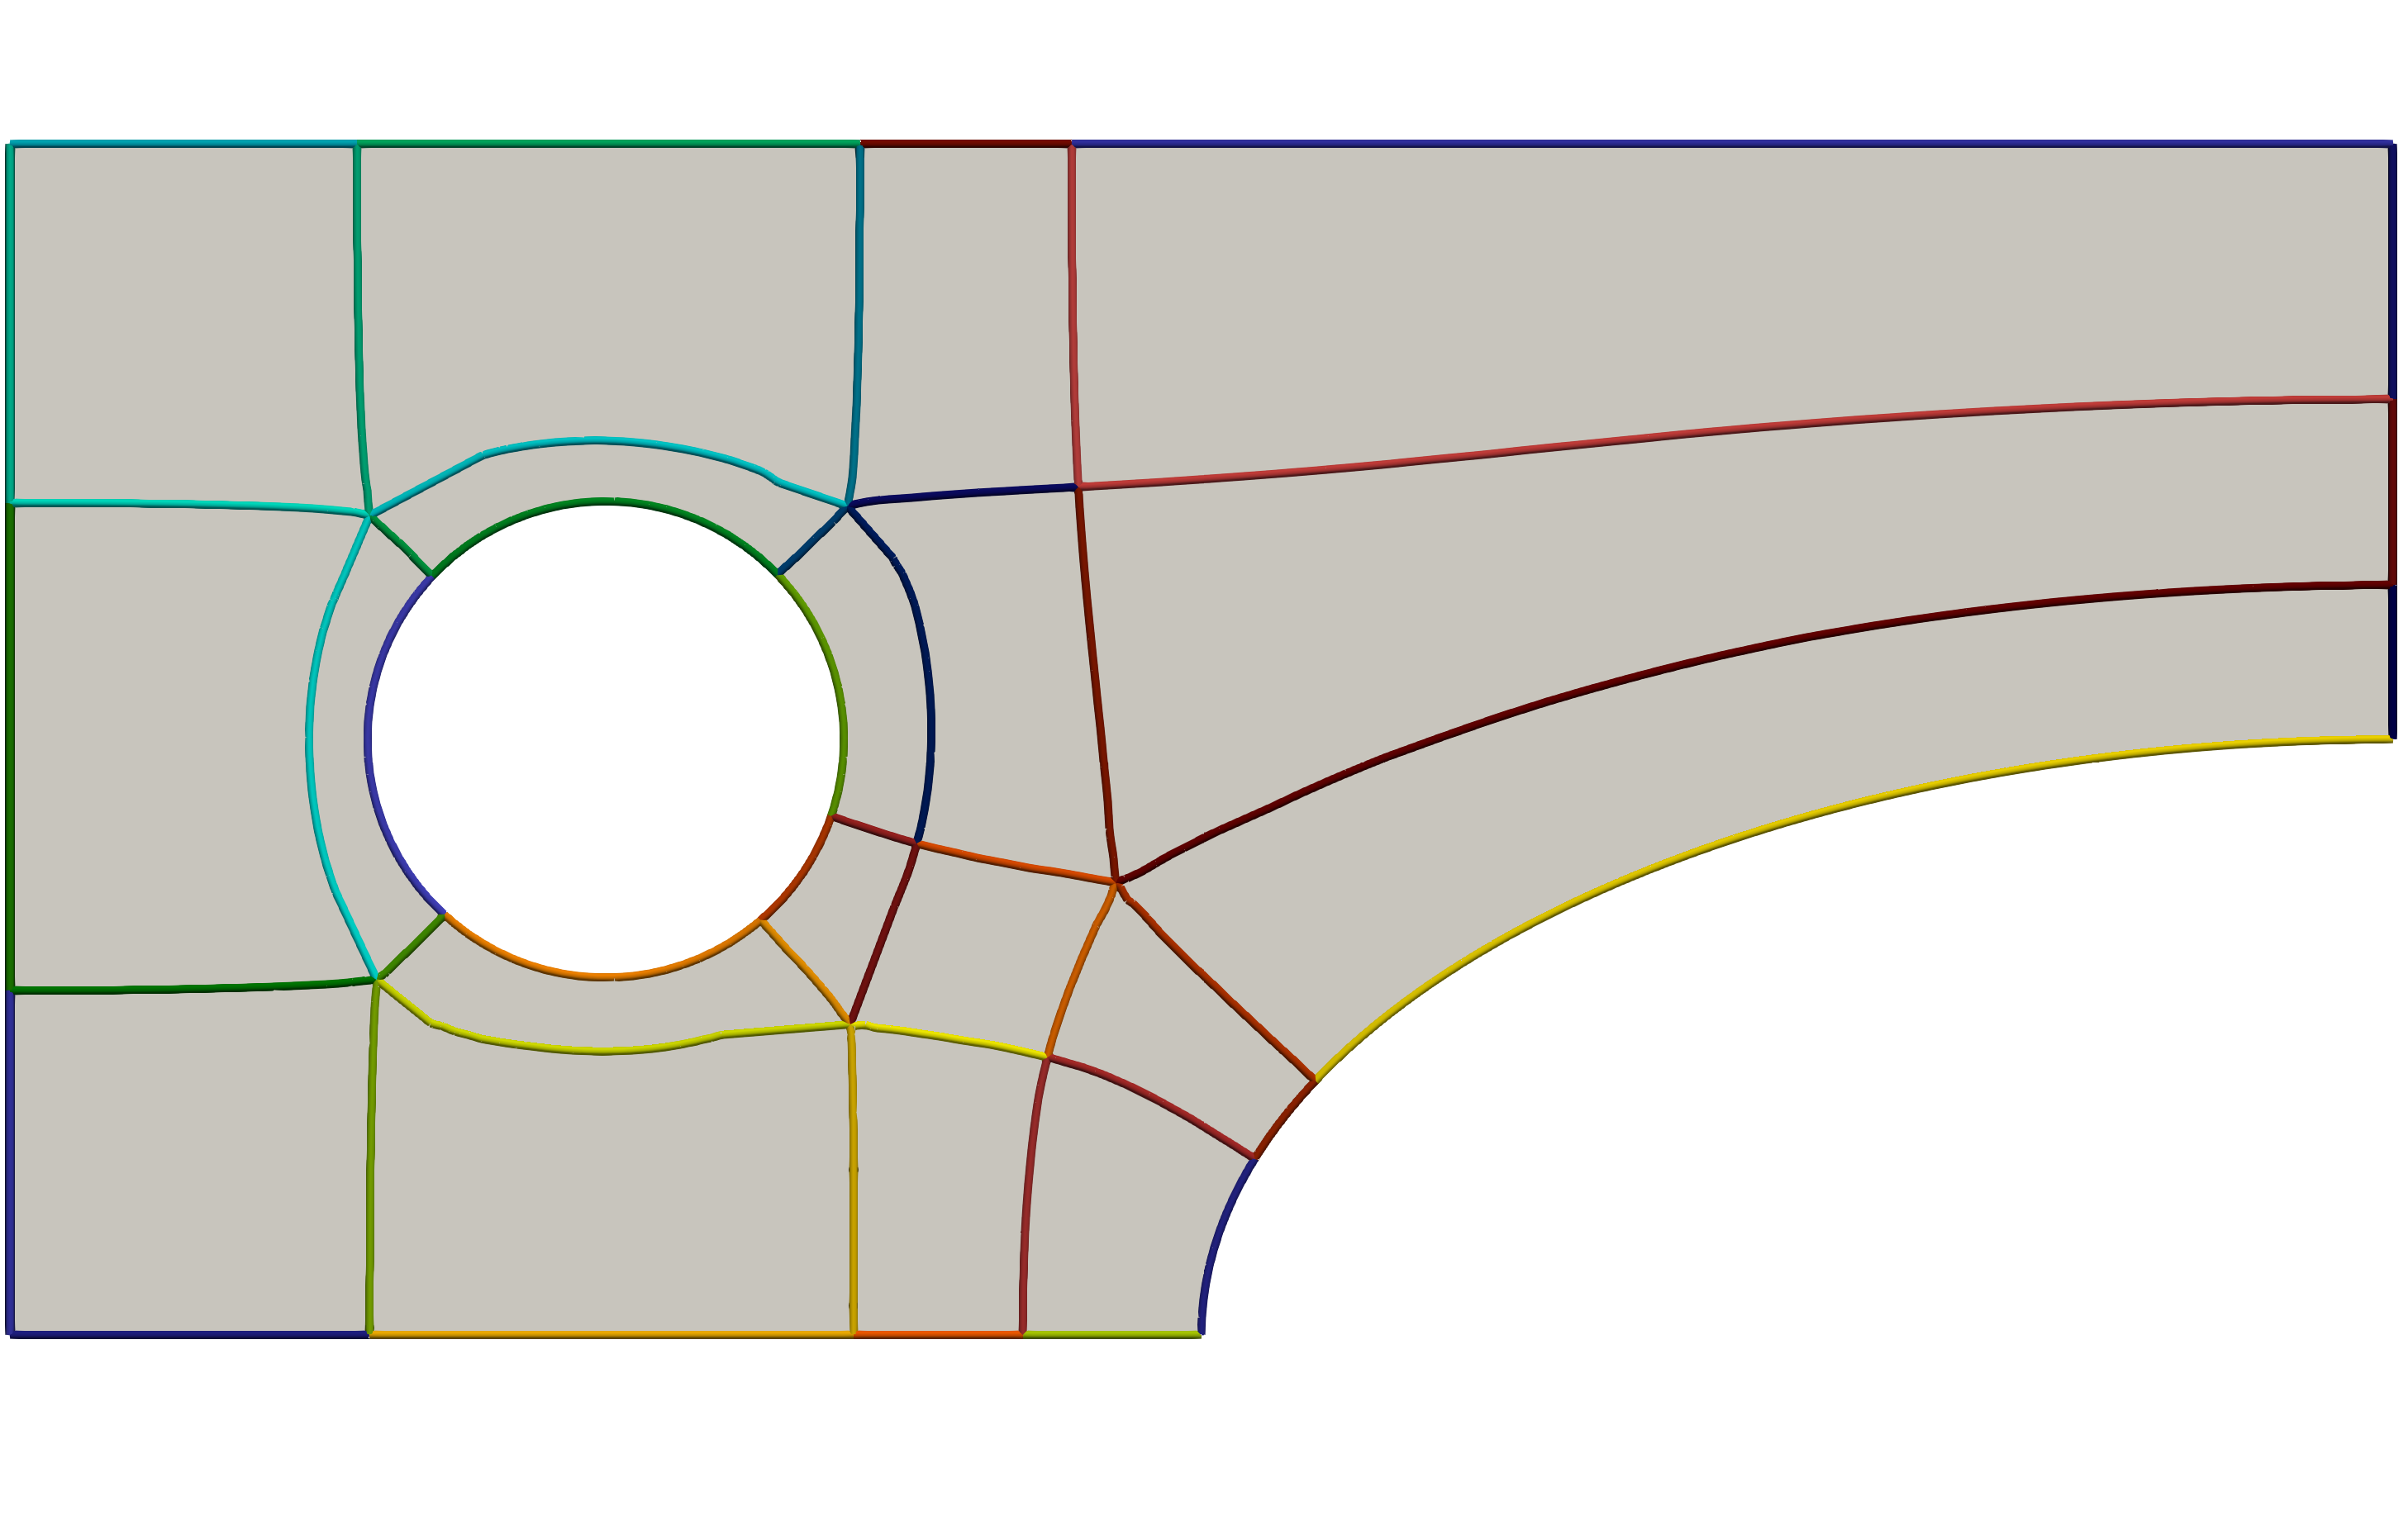
\includegraphics[width=10cm]
        {img/HIS-SingGraphOriginal-ConfusBallRad005.png}}
        \caption{ Mesh HIS - Singularity Graph}
      \end{figure}
		%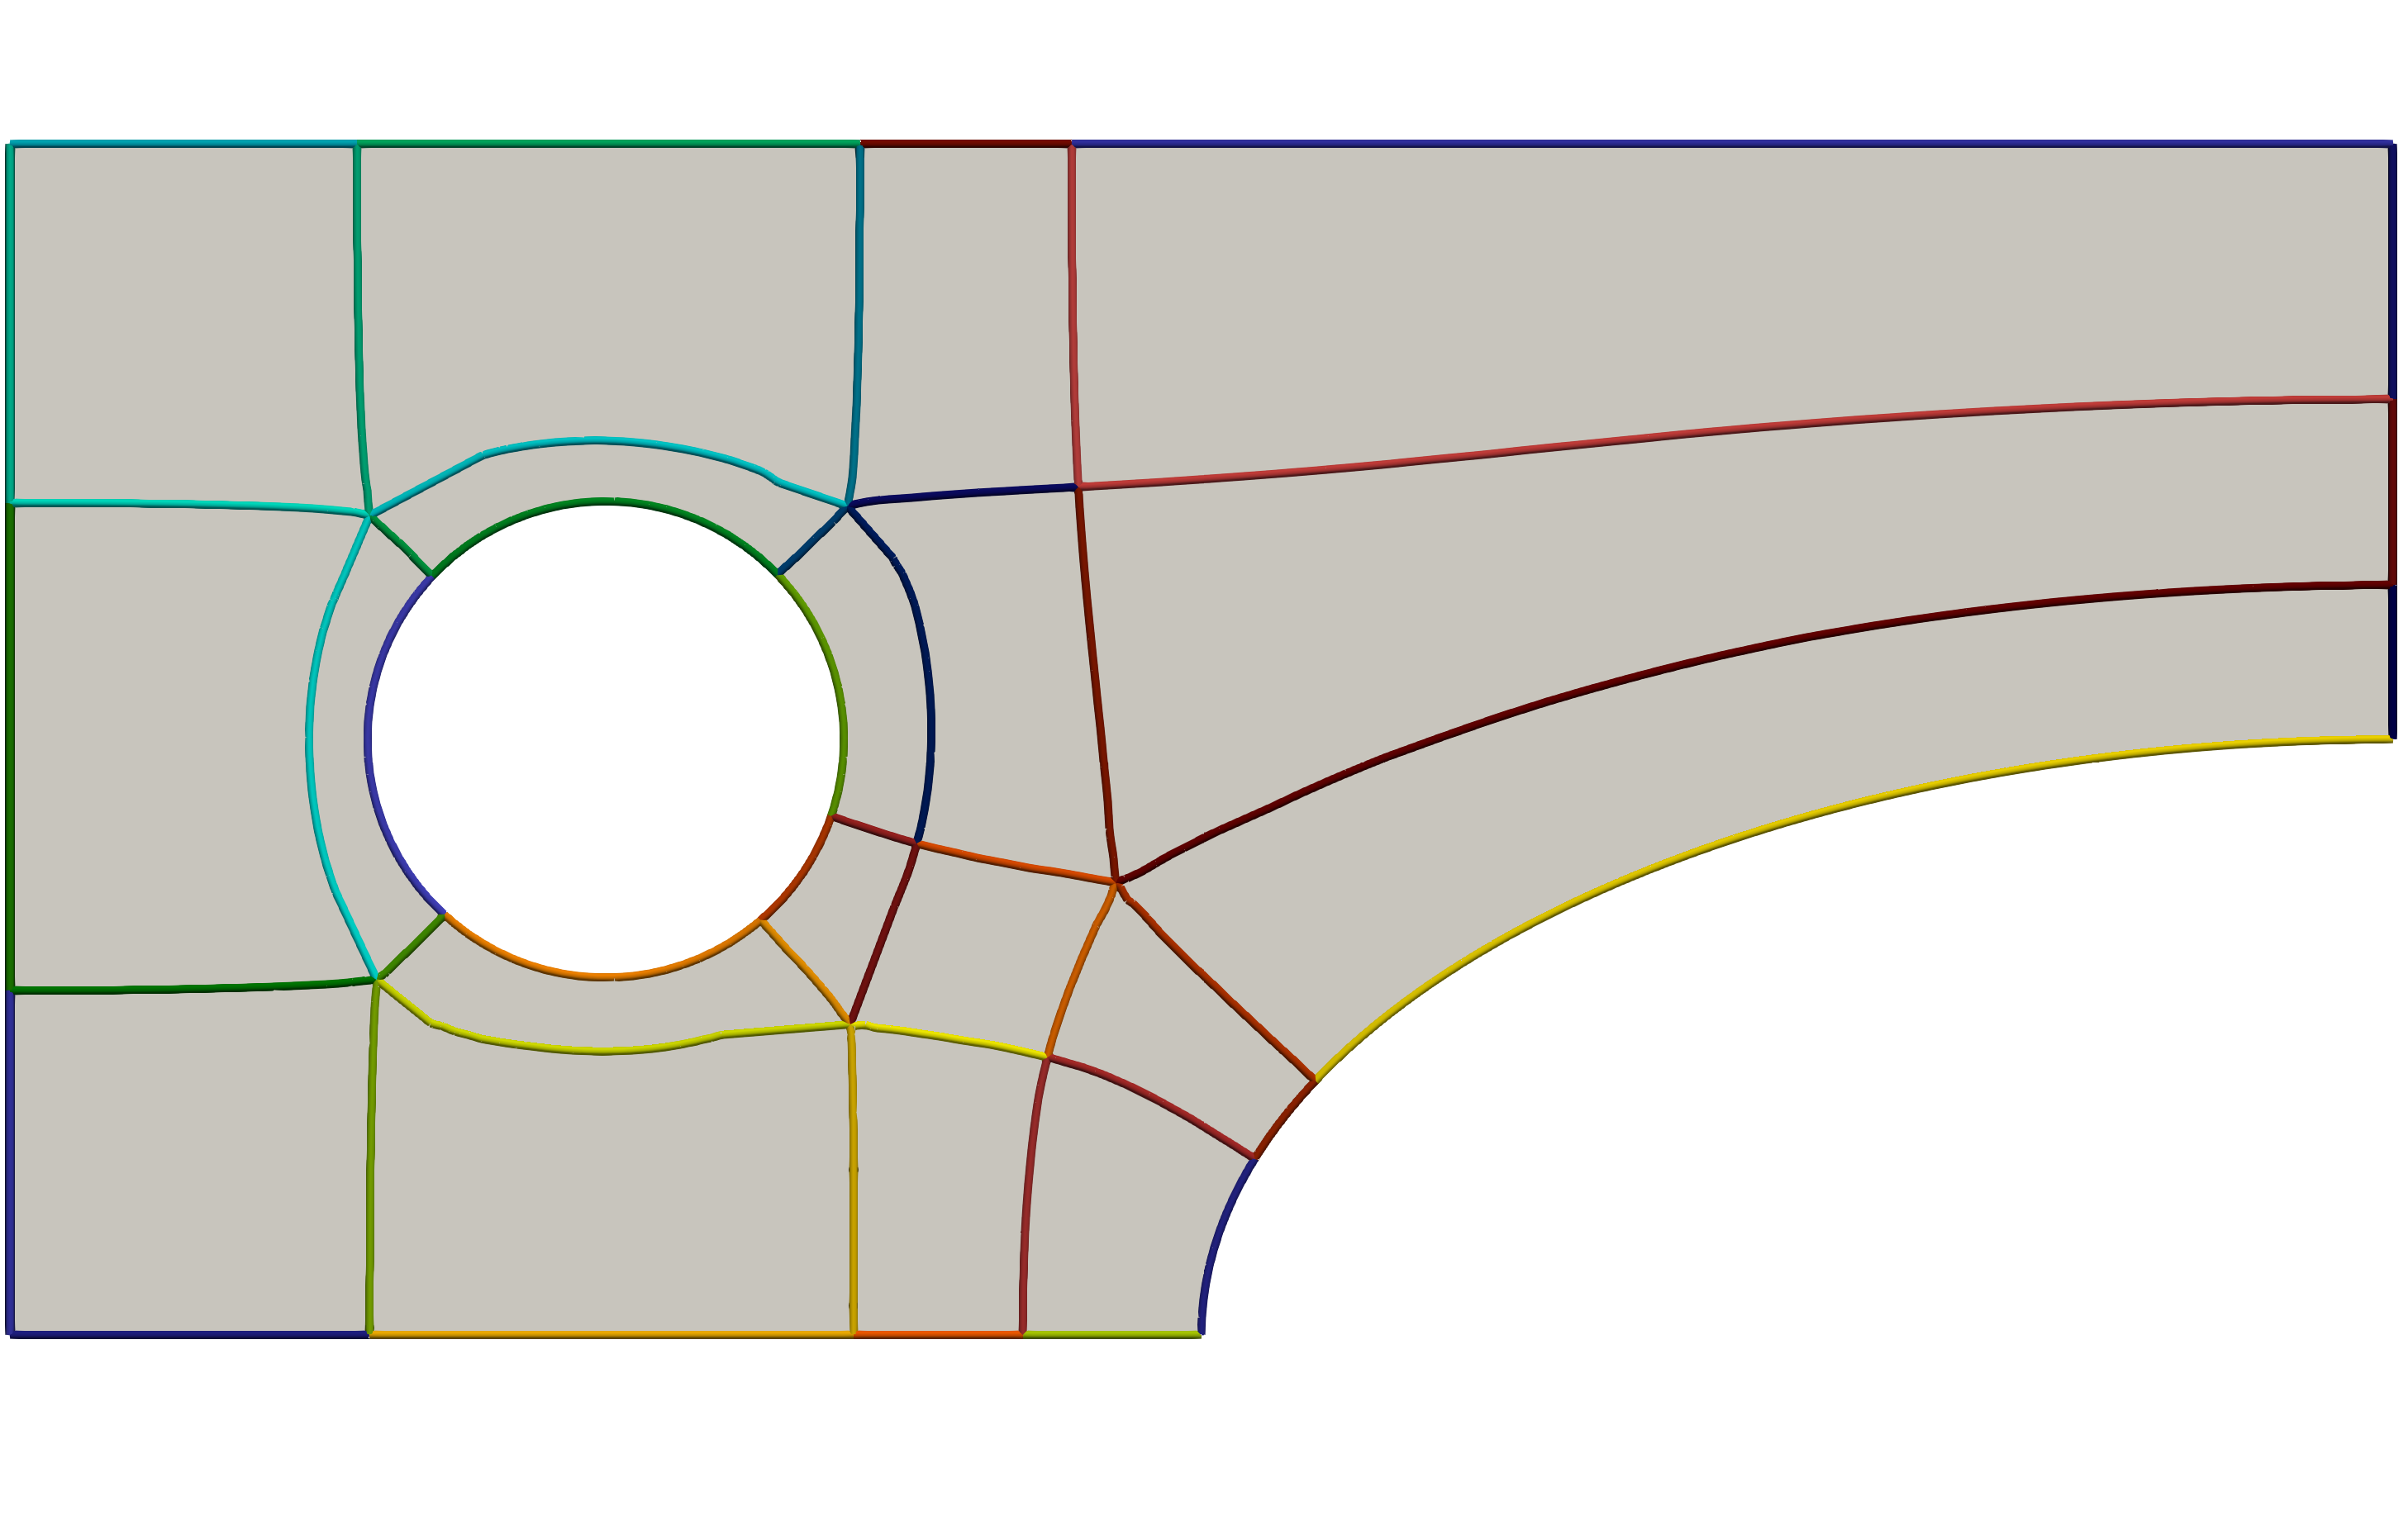
\includegraphics[height=7cm]{img/HIS-SingGraphOriginal-ConfusBallRad005.png}
	}
	
	%%%%%%%%%%%%%%%%%%%%%%%%%%%%%%%%%%%%%%%%%%%%%%%%%%%%%%%%%%%%%%%%%%%%%%%%%%%%%%%%%%%%%%%%
	\frame{
		\frametitle{Overall Algorithm Steps}	
		\begin{itemize}			
			\item 3. Remesh resulted quad patches 
		\end{itemize}
		\begin{figure}[]
        \center{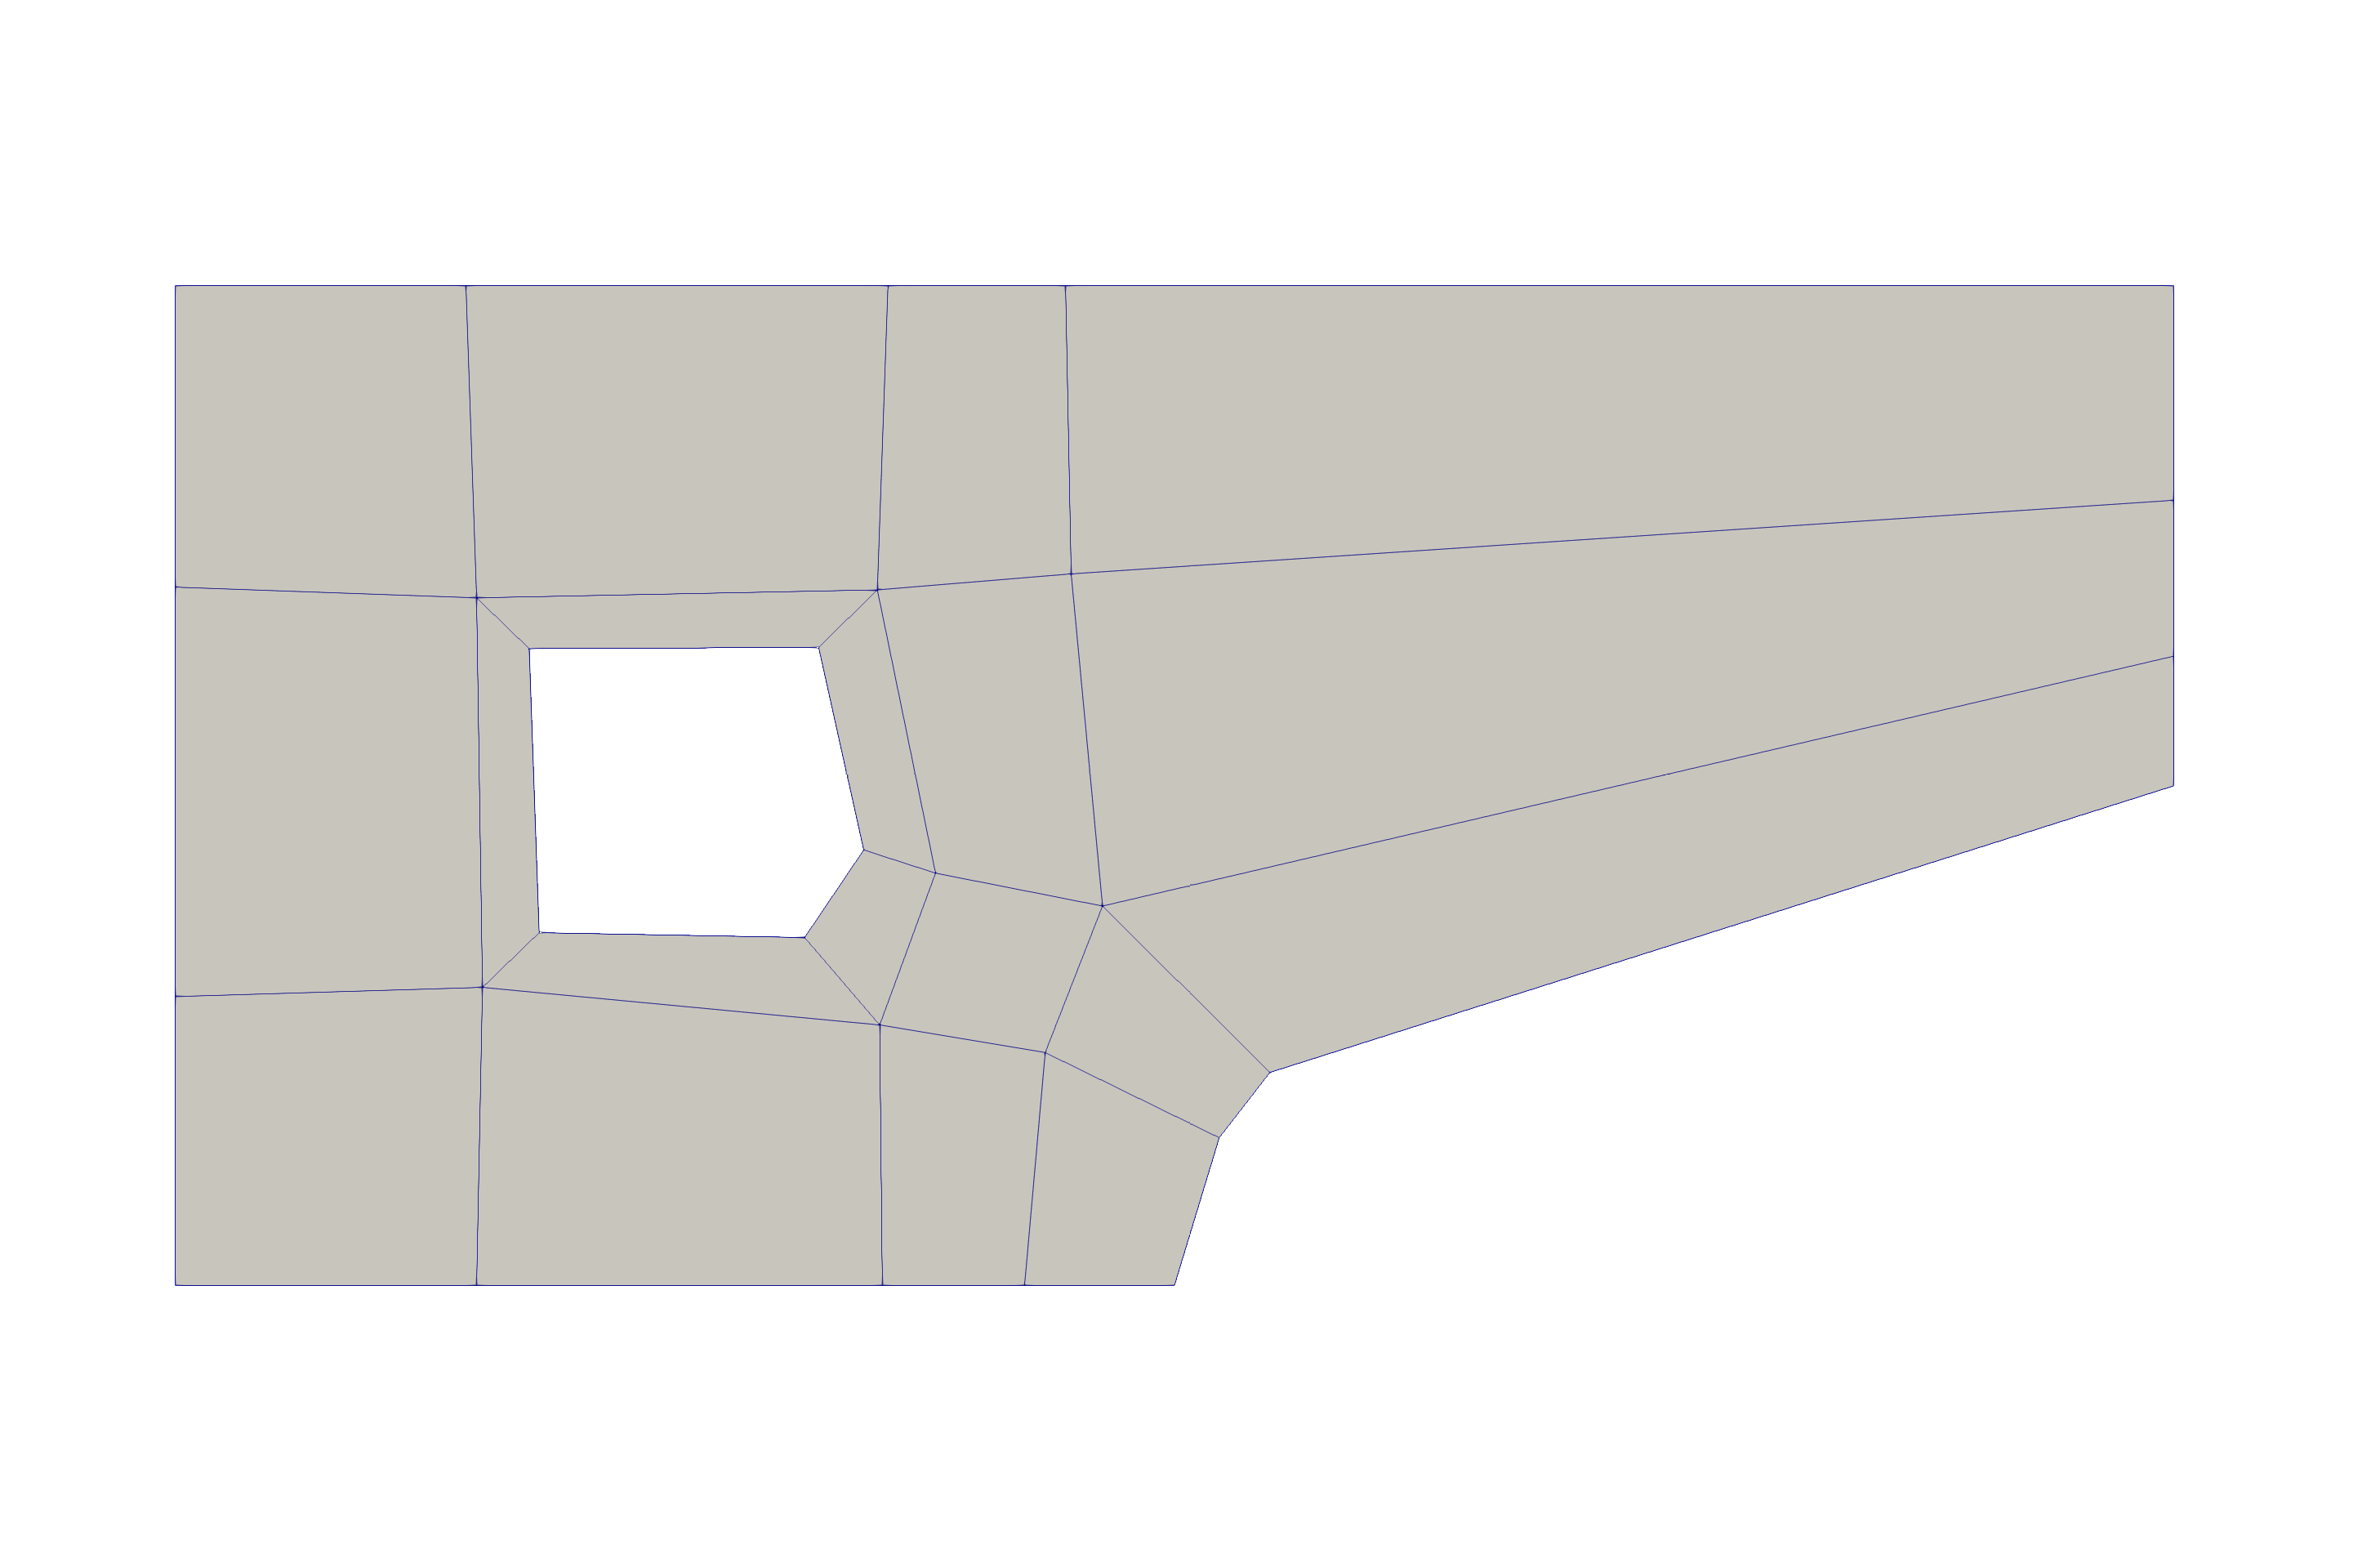
\includegraphics[width=10cm]
        {img/HIS-patches.png}}
        \caption{ Mesh HIS - Patches}
      \end{figure}
		%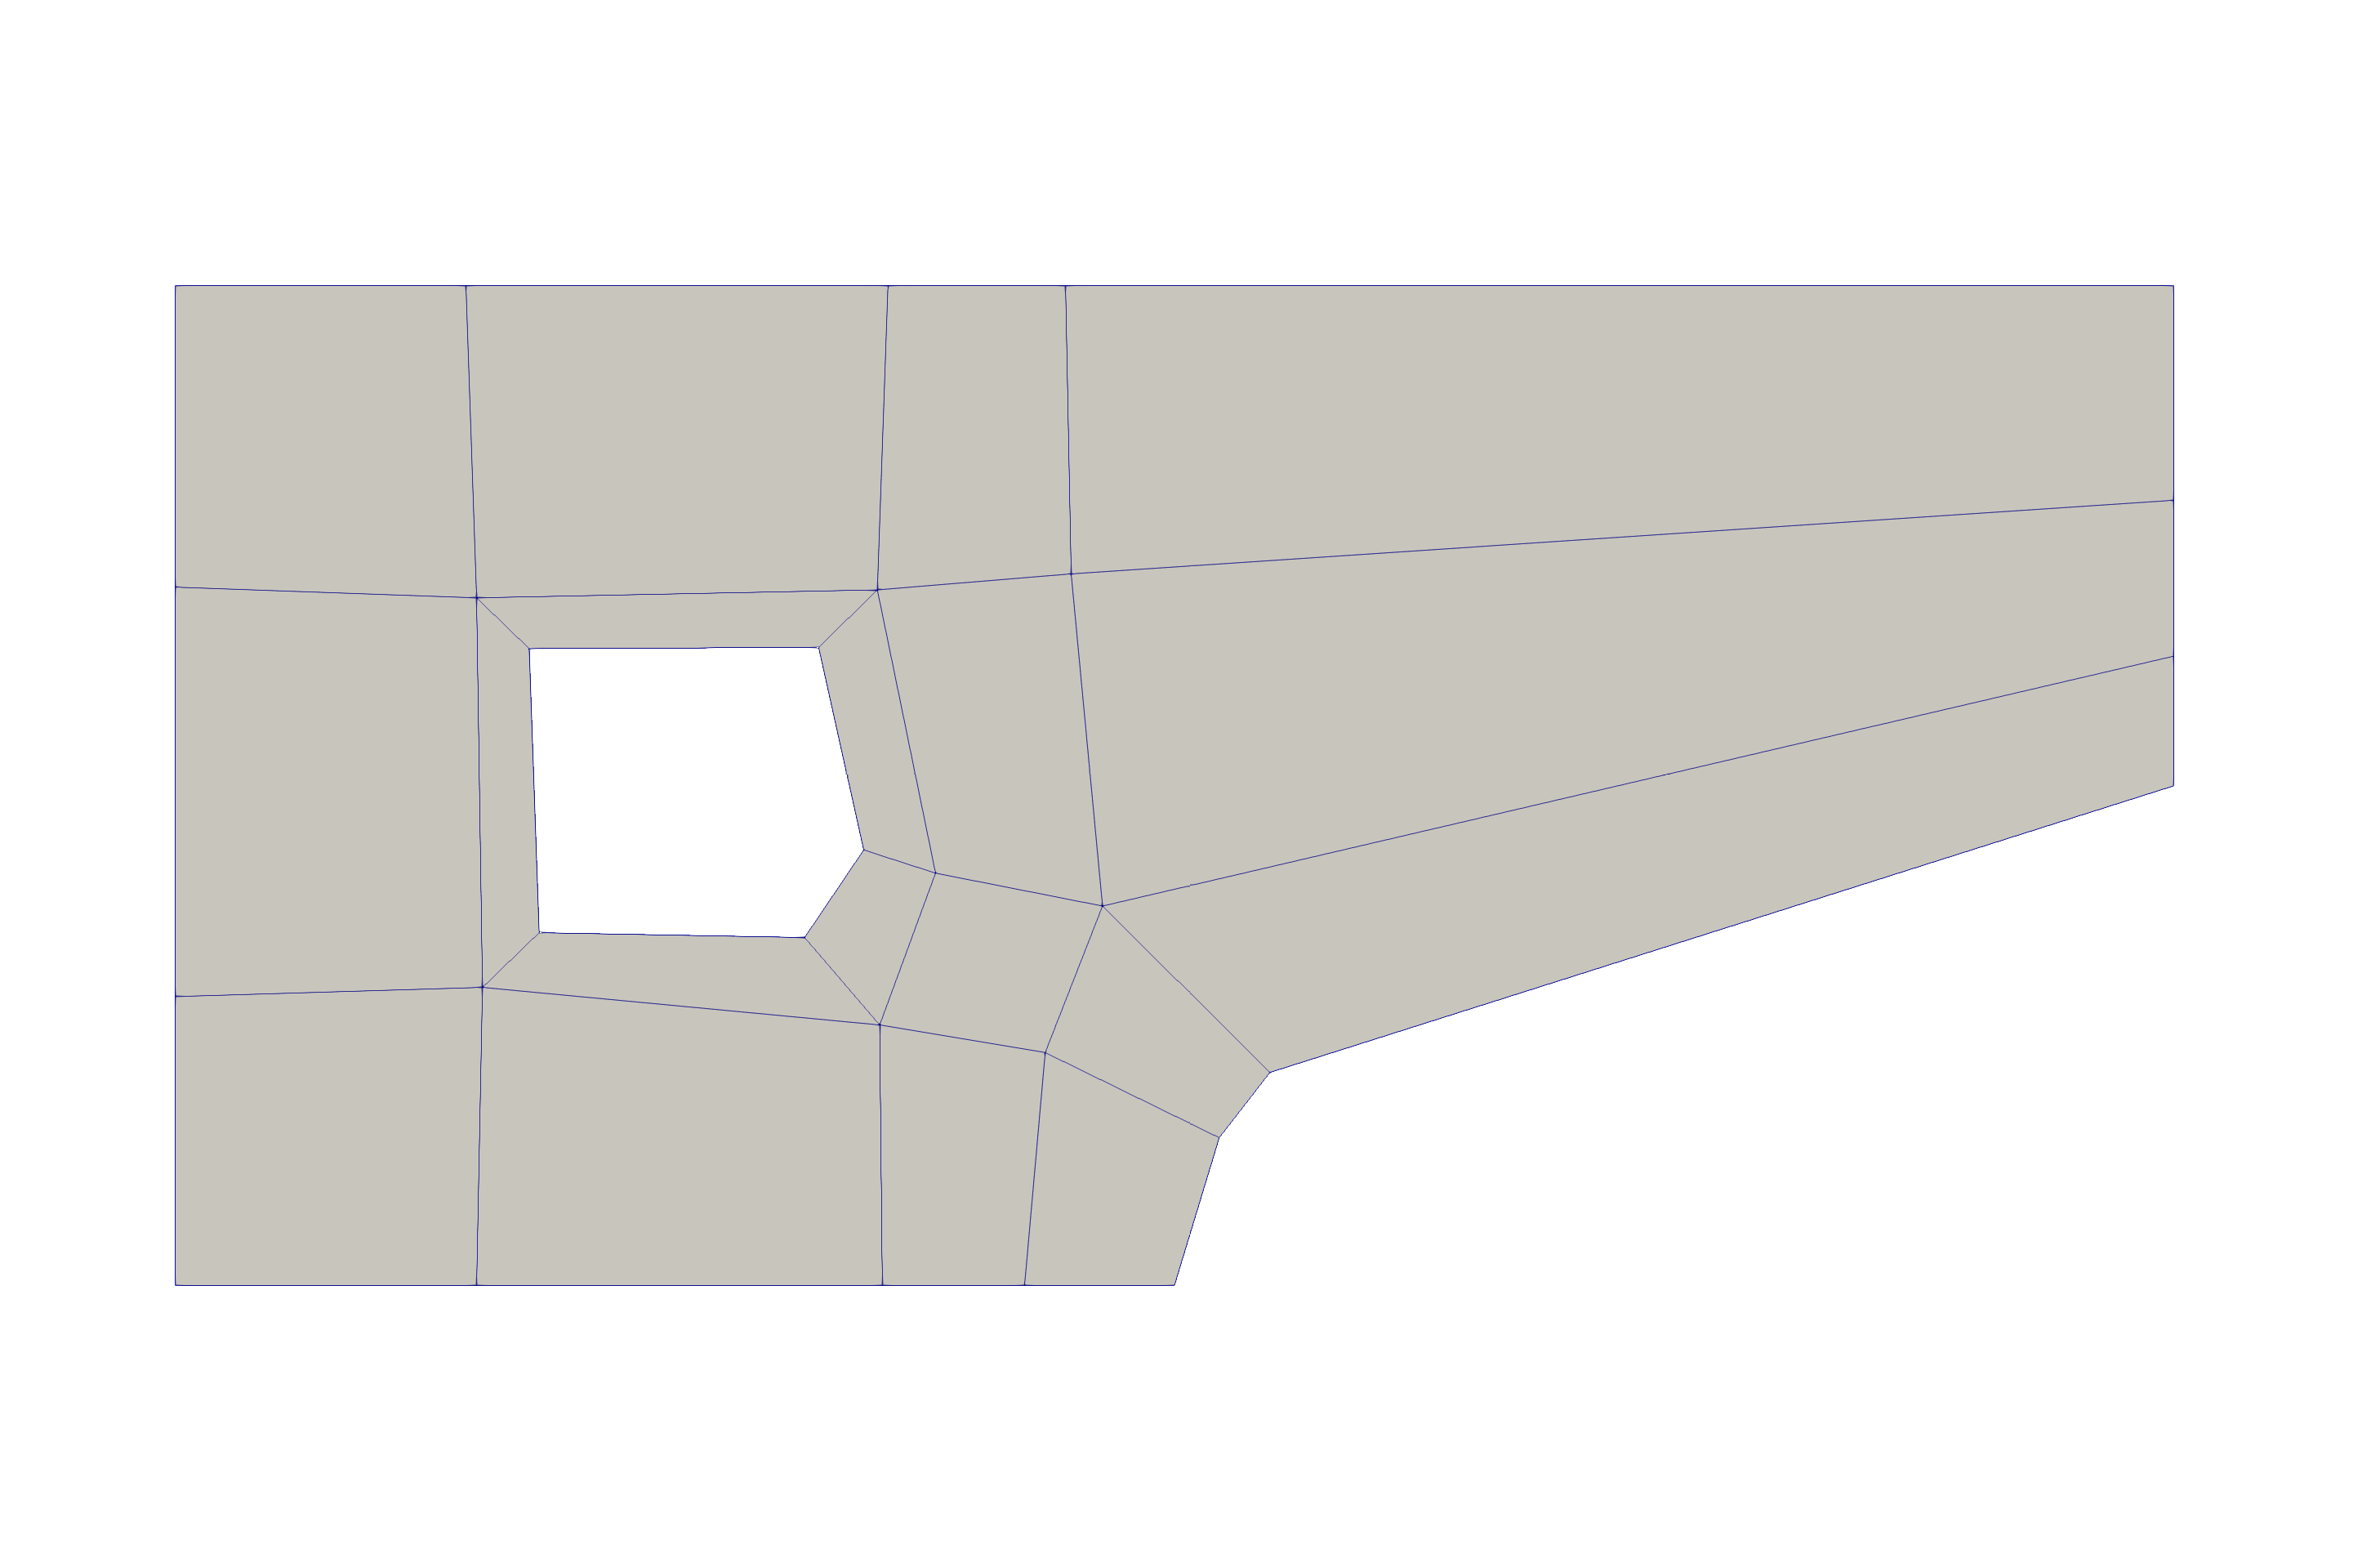
\includegraphics[height=7cm]{img/HIS-patches.png}
	}
	
	
	%%%%%%%%%%%%%%%%%%%%%%%%%%%%%%%%%%%%%%%%%%%%%%%%%%%%%%%%%%%%%%%%%%%%%%%%%%%%%%%%%%%%%%%%
	
	\frame {
		\frametitle{Singularity Graph Building}			
		%\[\frac{-b \pm \sqrt{b^2 - c}}{2a}\]		
		\begin{itemize}
			\item Detect singular triangles and their slots
			\begin{figure}[]
        \center{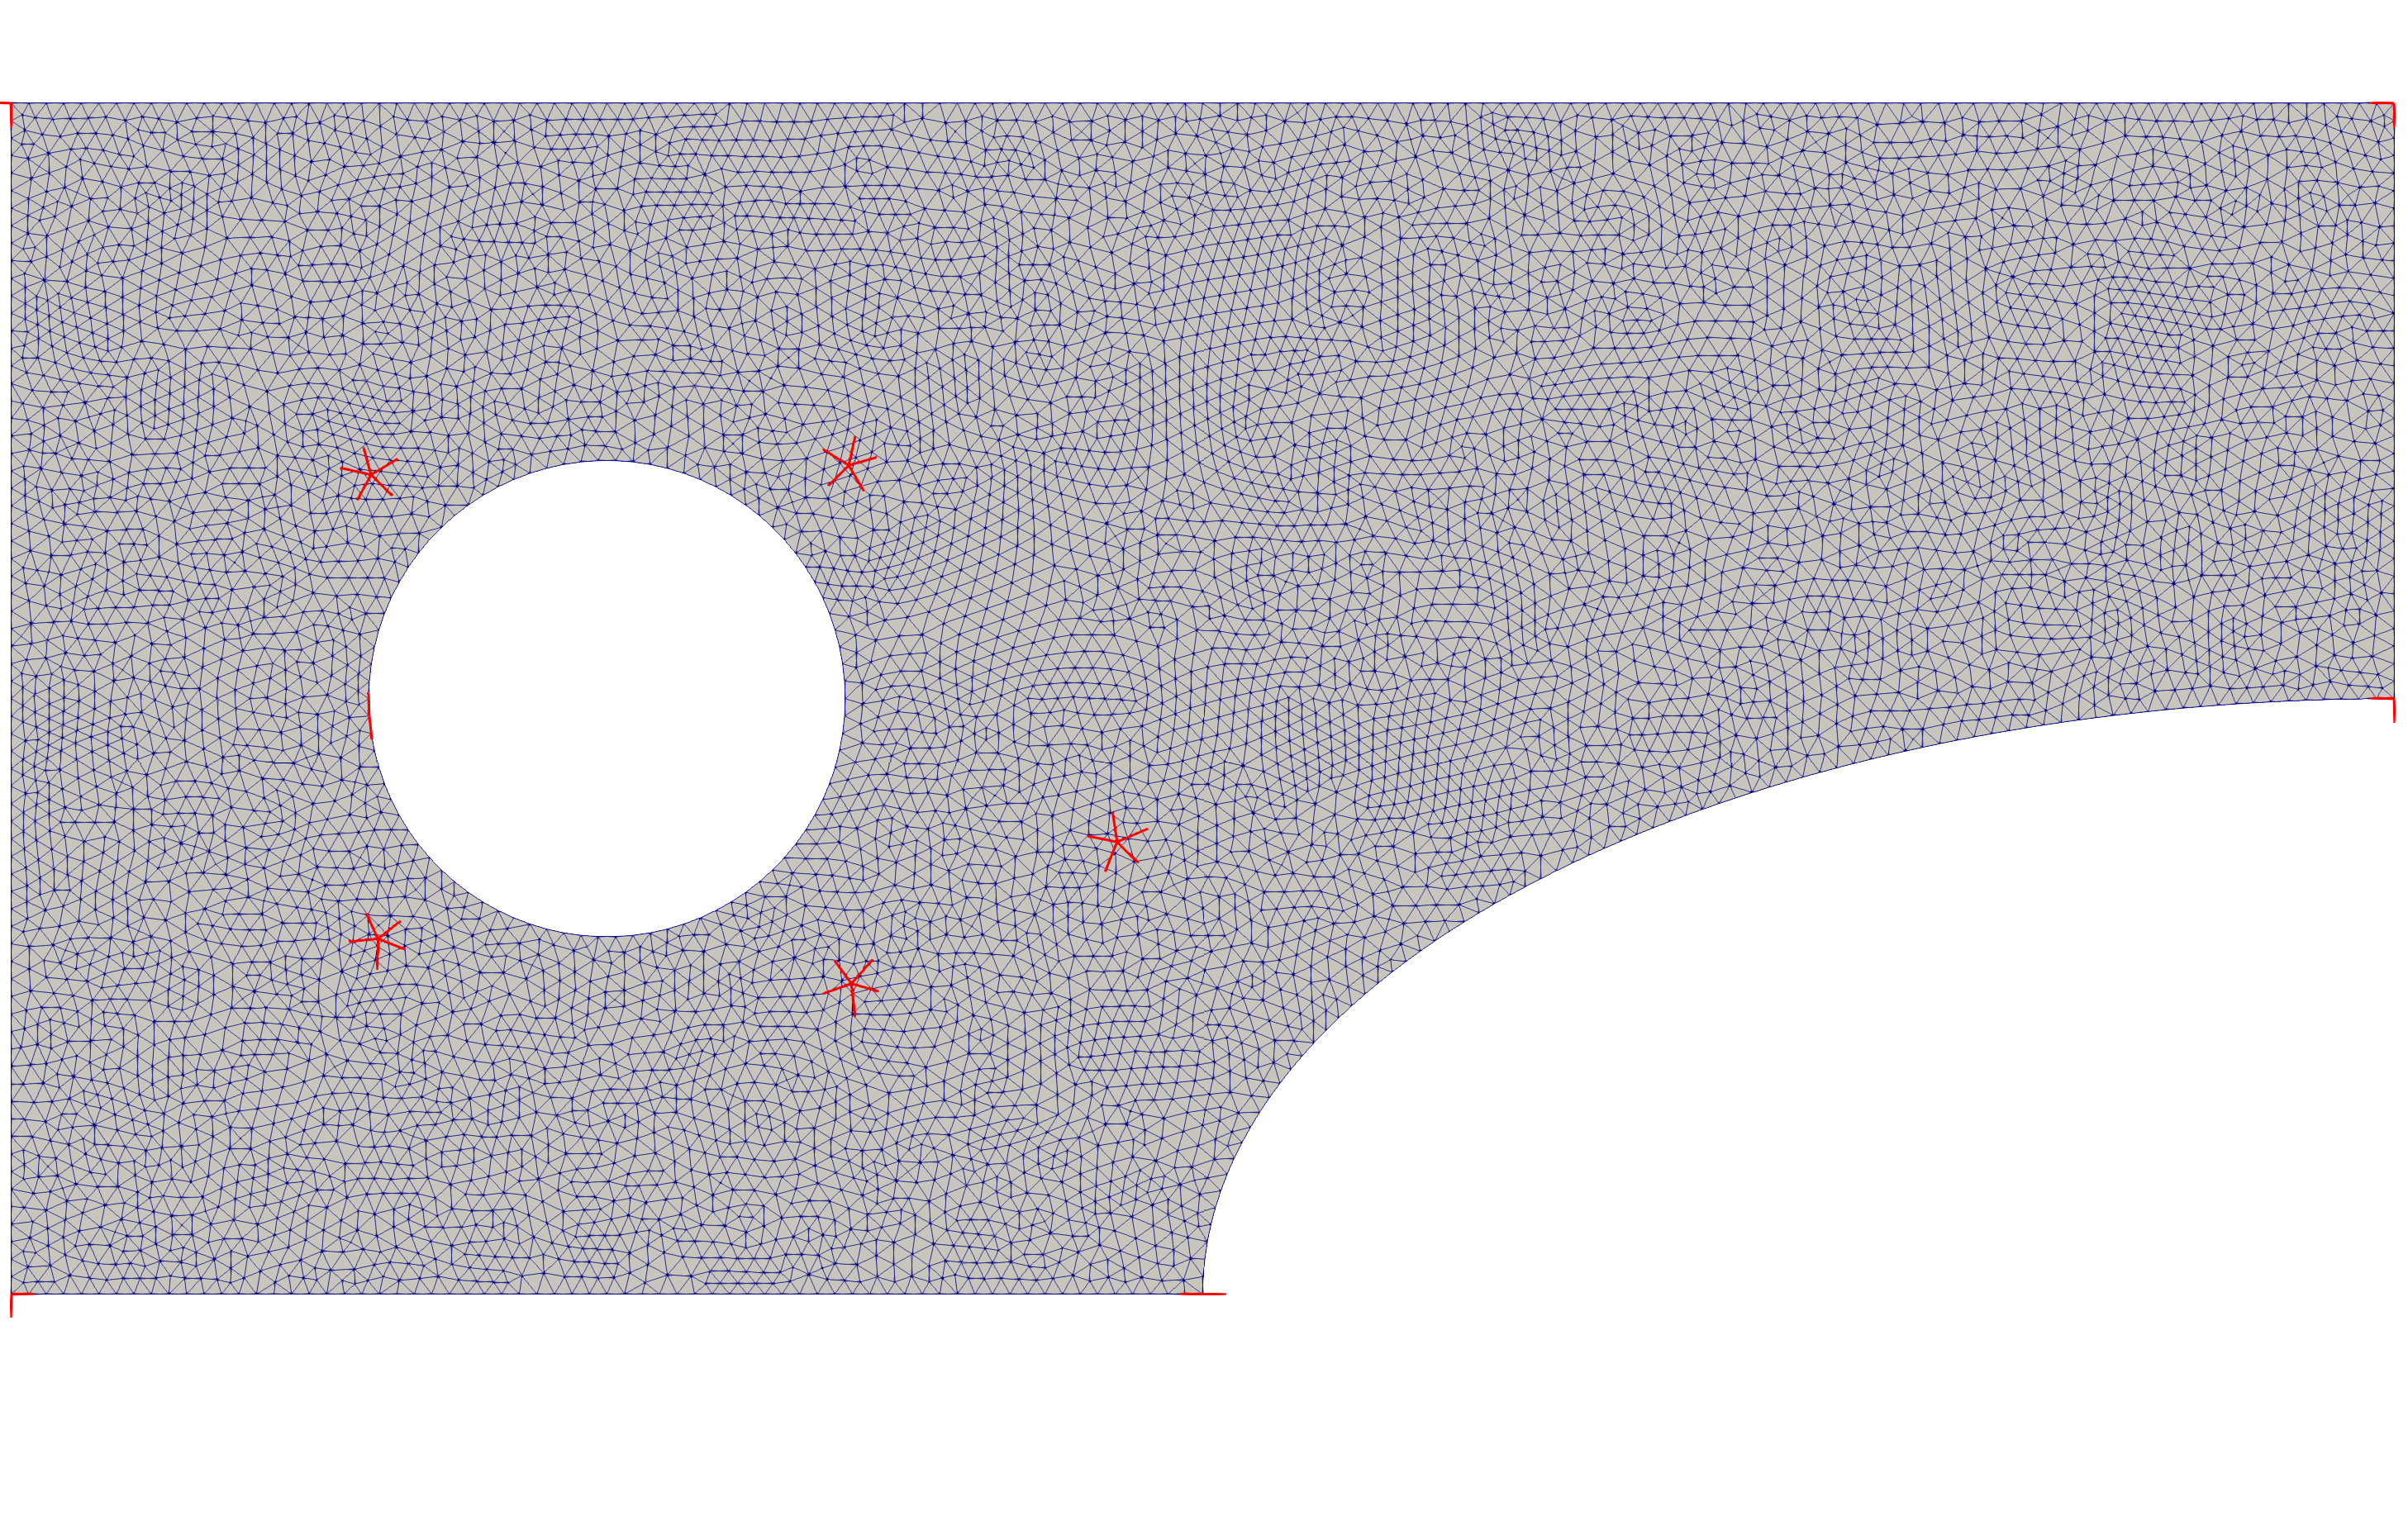
\includegraphics[width=10cm]
        {img/HIS-Slots.png}}
        \caption{ Mesh HIS - Singularity Slots}
      \end{figure}
			%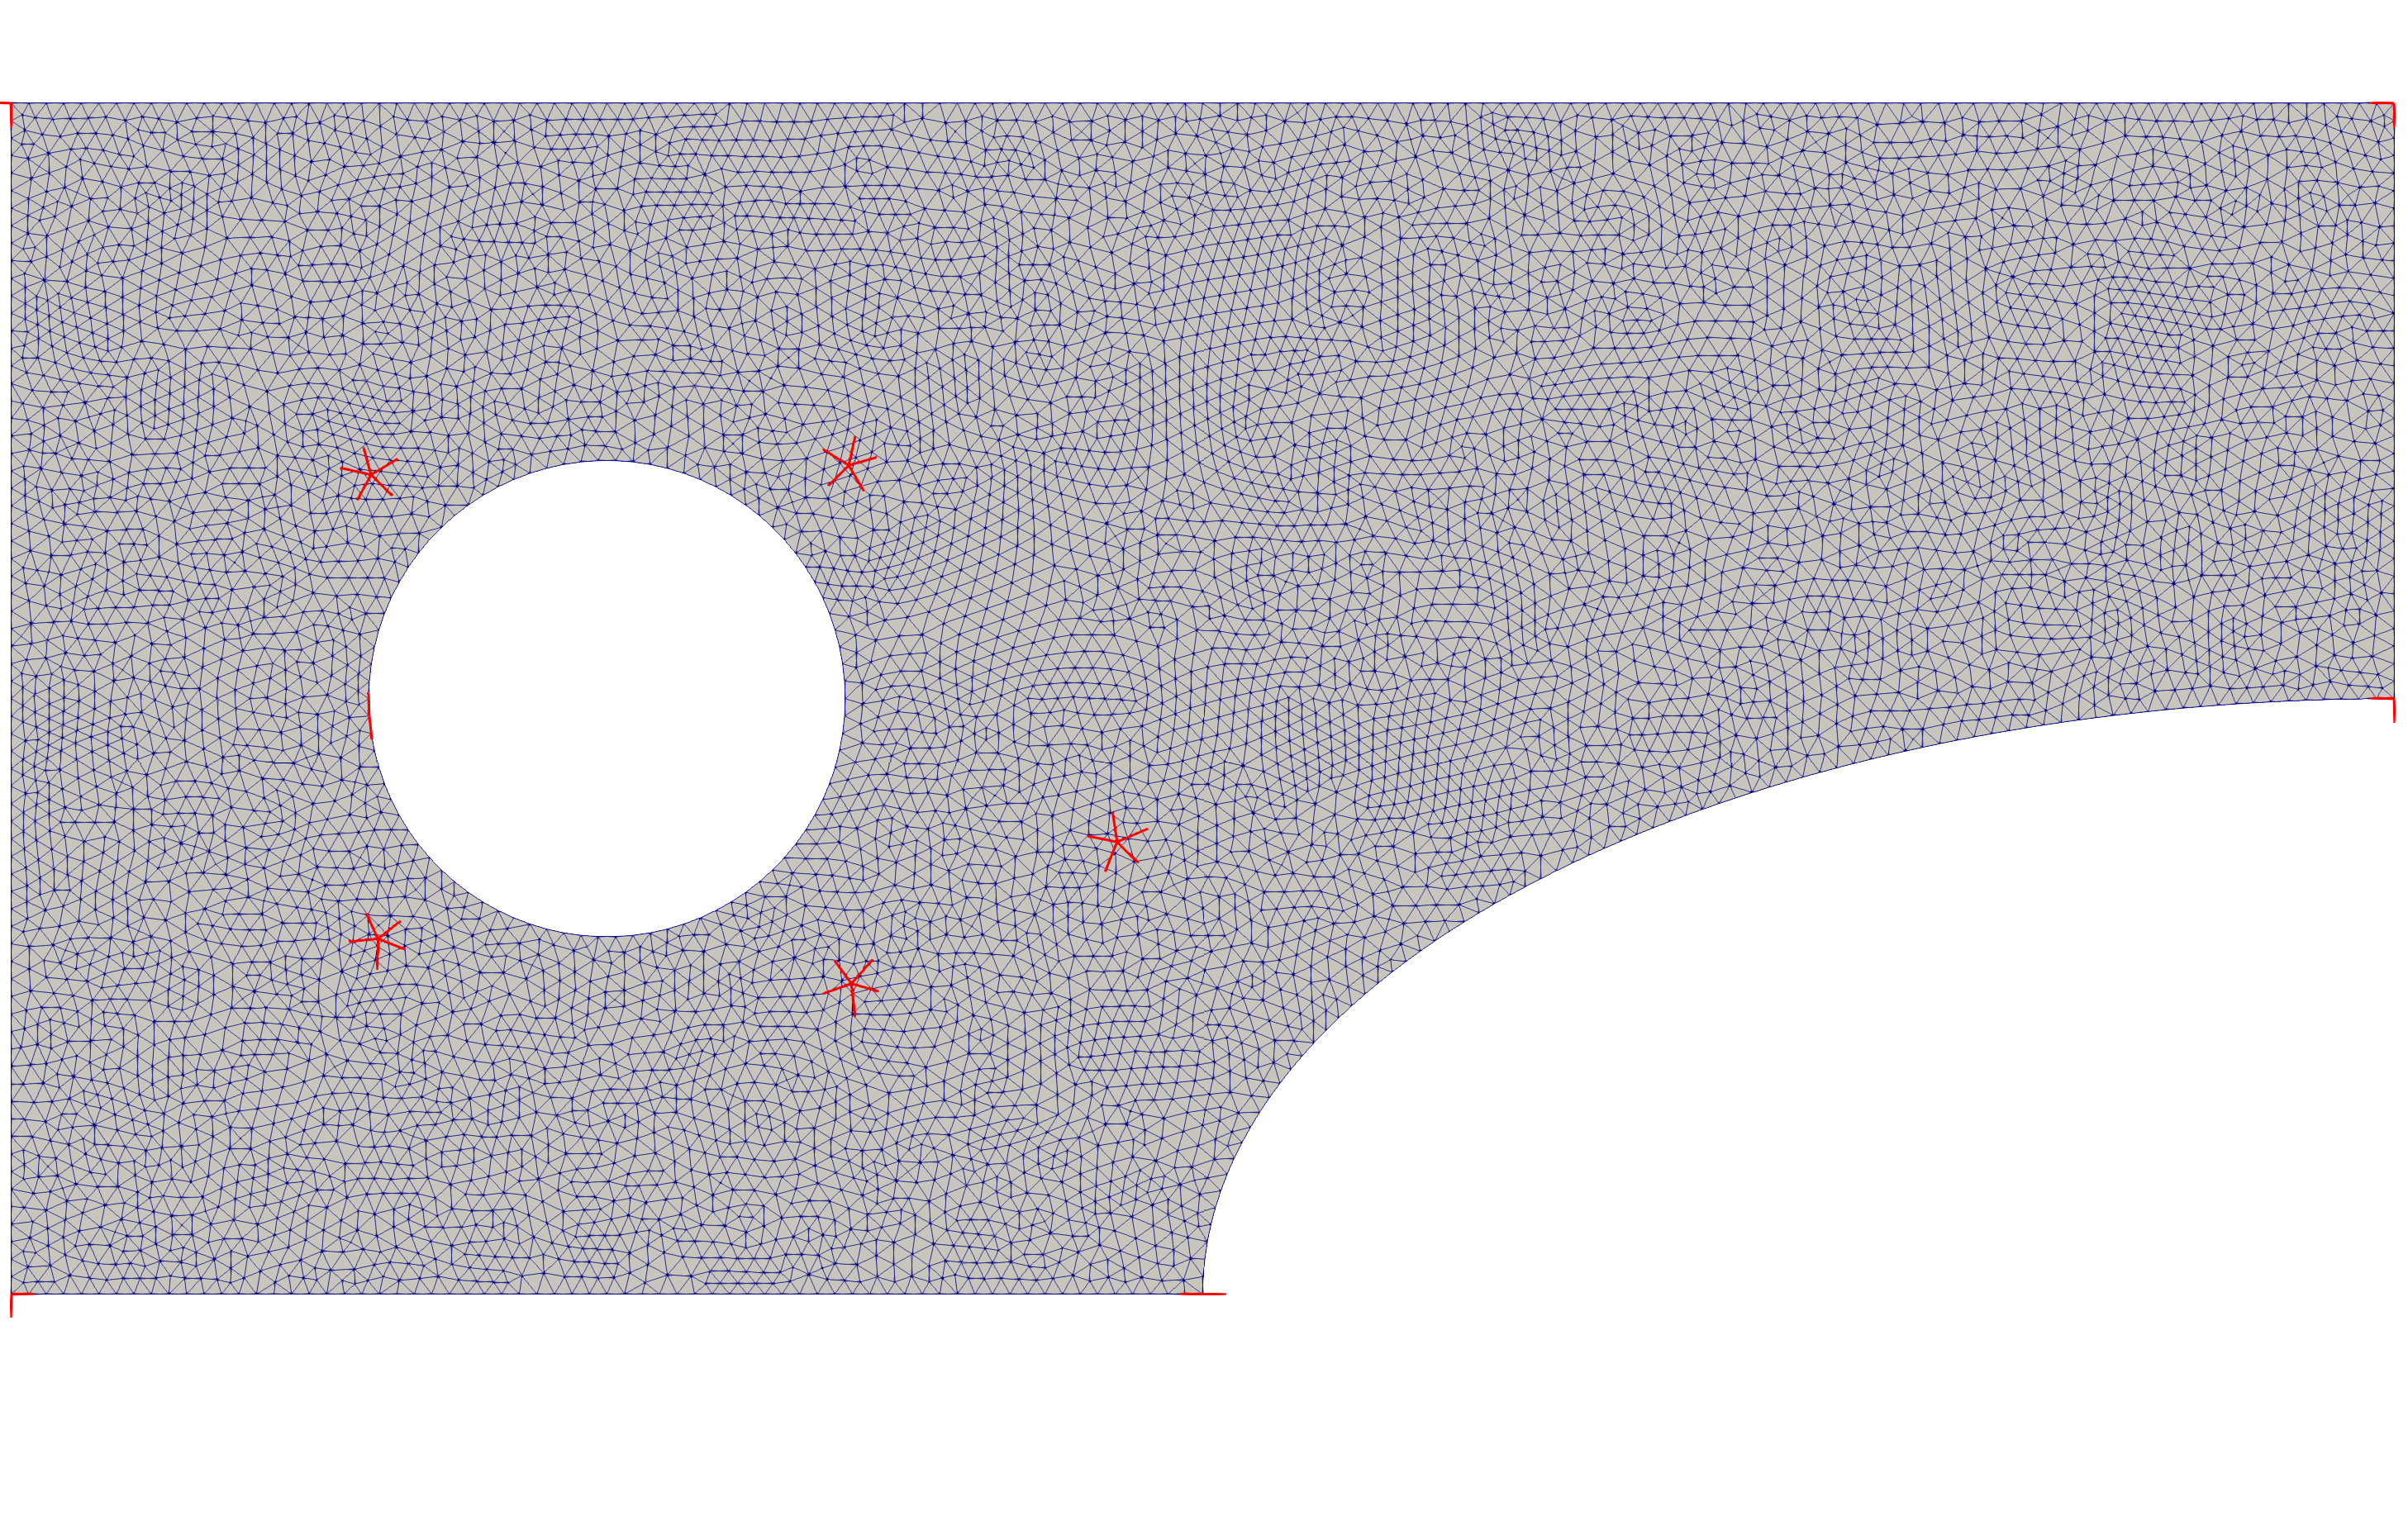
\includegraphics[height=7cm]{img/HIS-Slots.png}
			
		\end{itemize}
	}
	
	%%%%%%%%%%%%%%%%%%%%%%%%%%%%%%%%%%%%%%%%%%%%%%%%%%%%%%%%%%%%%%%%%%%%%%%%%%%%%%%%%%%%%%%%
	\frame {
		\frametitle{Singularity Graph Building}			
		%\[\frac{-b \pm \sqrt{b^2 - c}}{2a}\]		
		\begin{itemize}
			\item Detect singular triangles and their slots	
			\begin{figure}[]
        \center{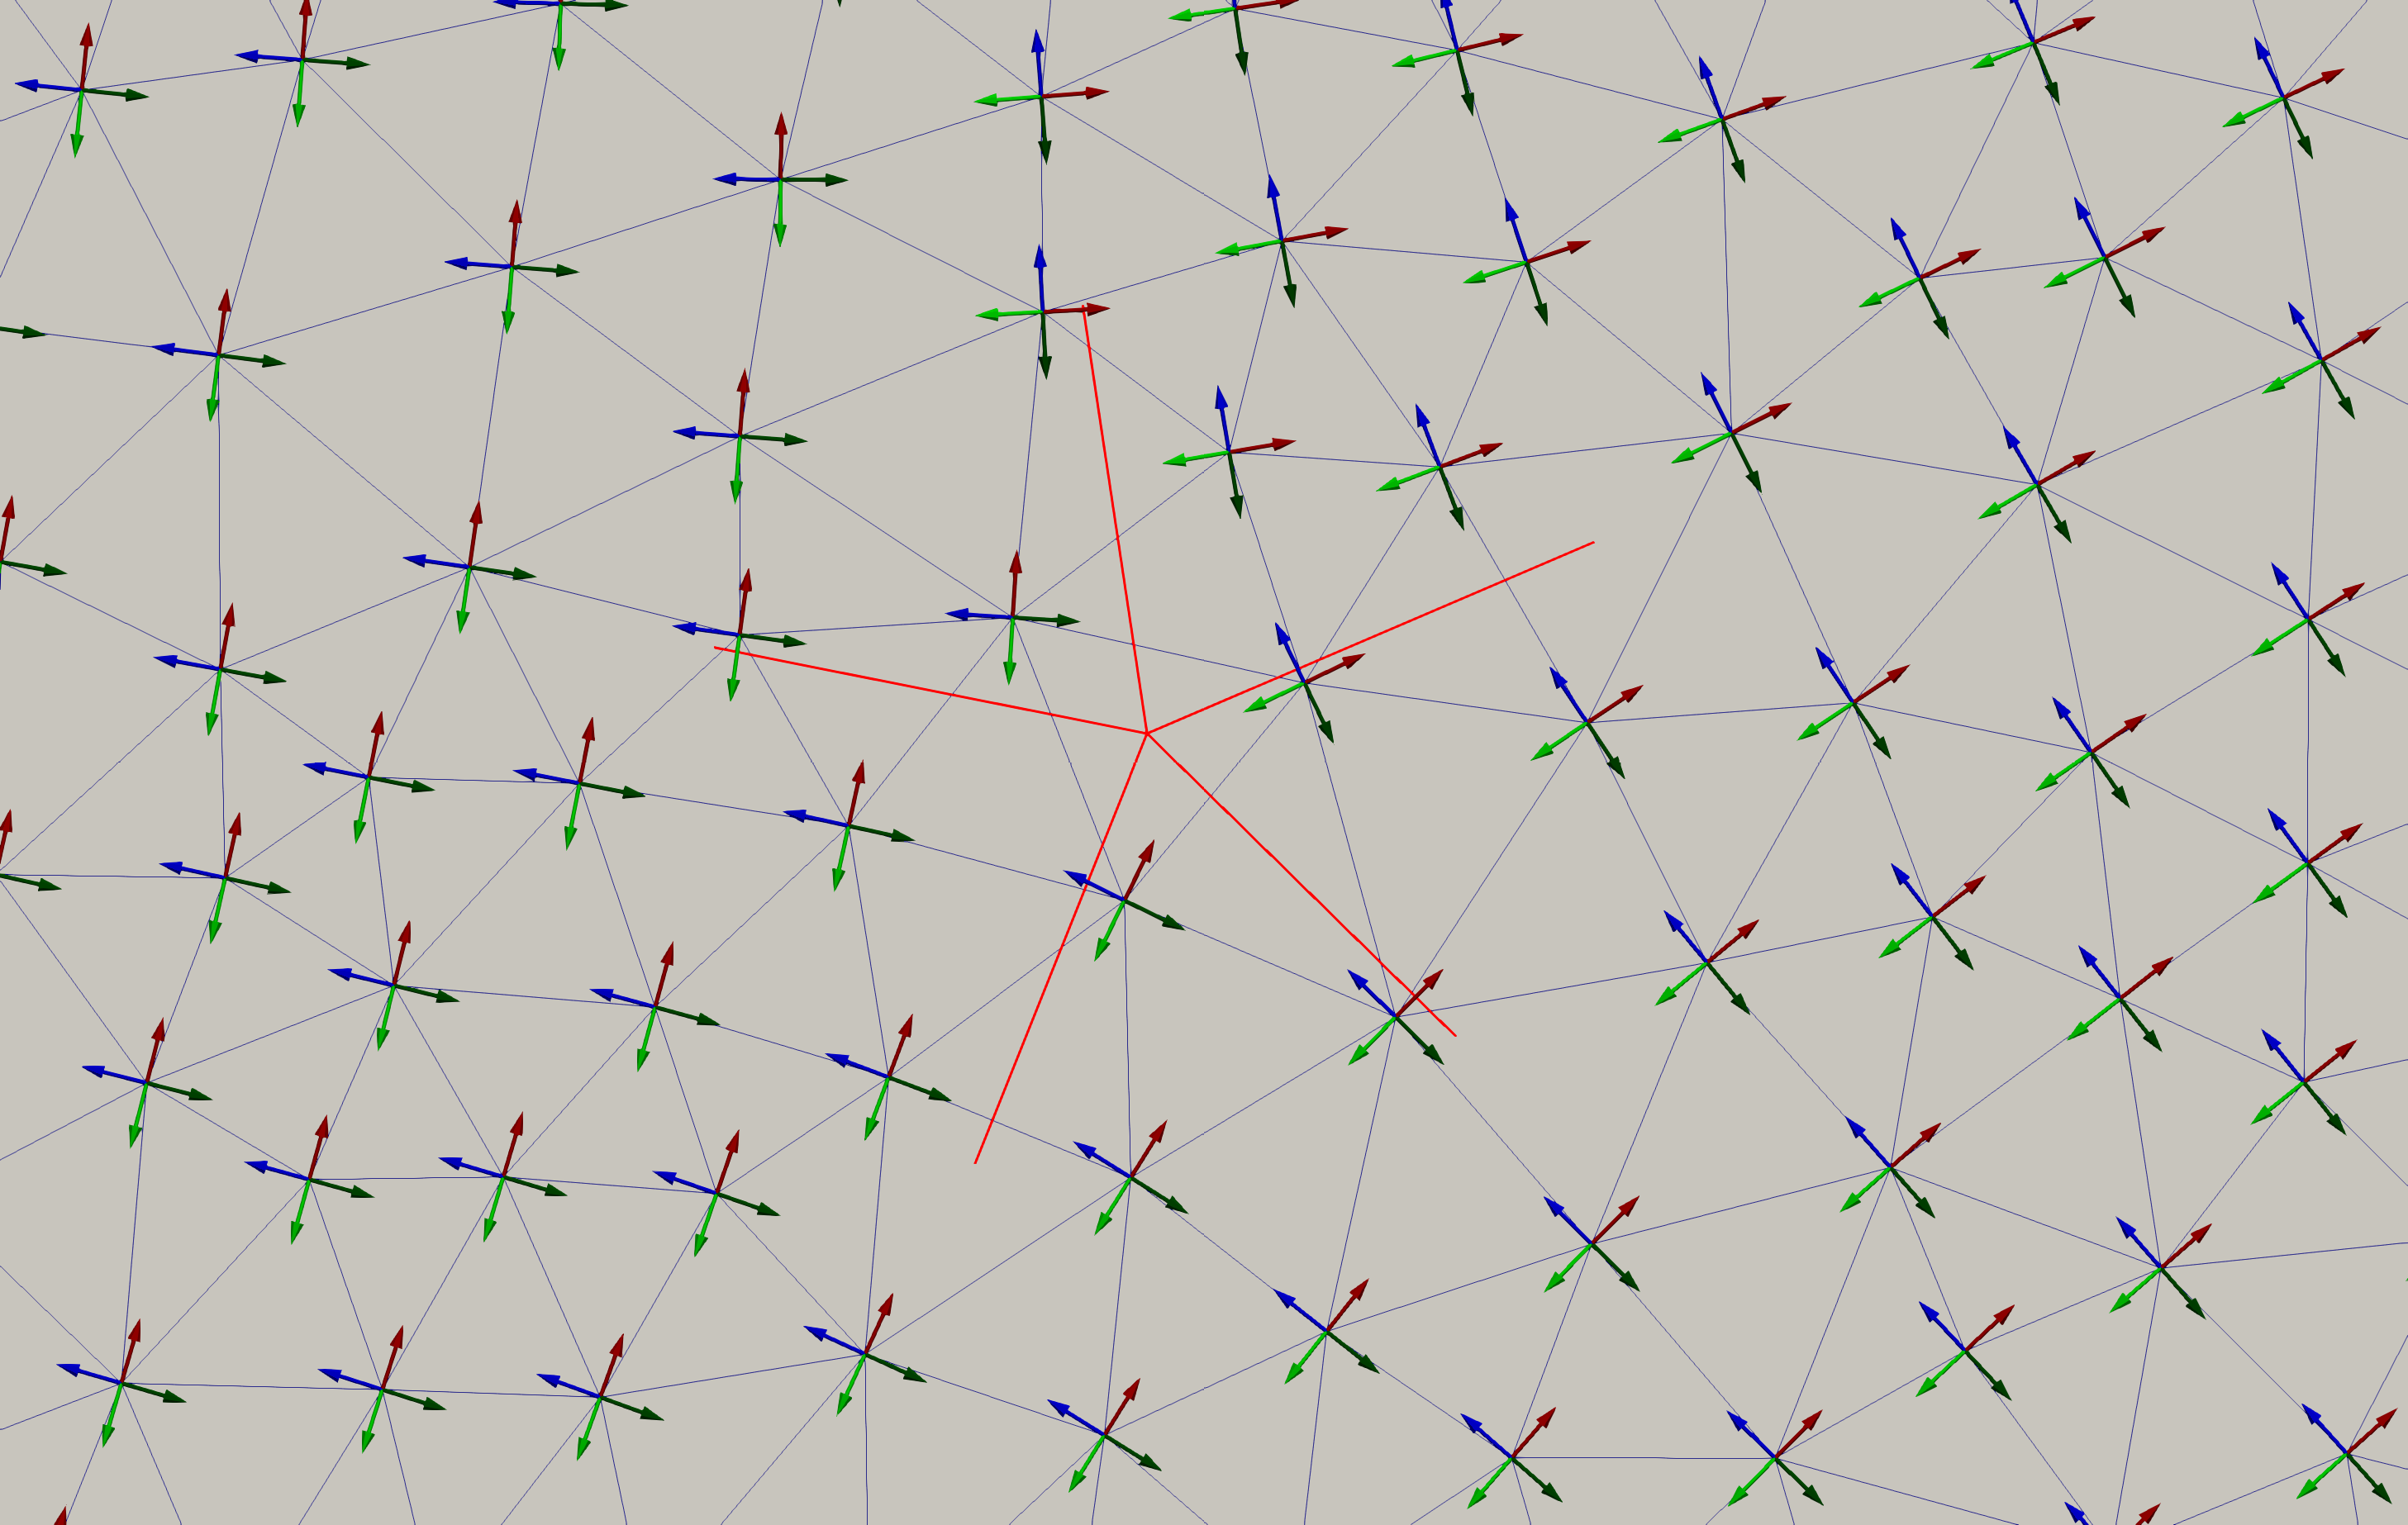
\includegraphics[width=10cm]
        {img/HIS-Slots-close-up.png}}
        \caption{ Mesh HIS - Singularity Slots - close-up}
      \end{figure}		
			%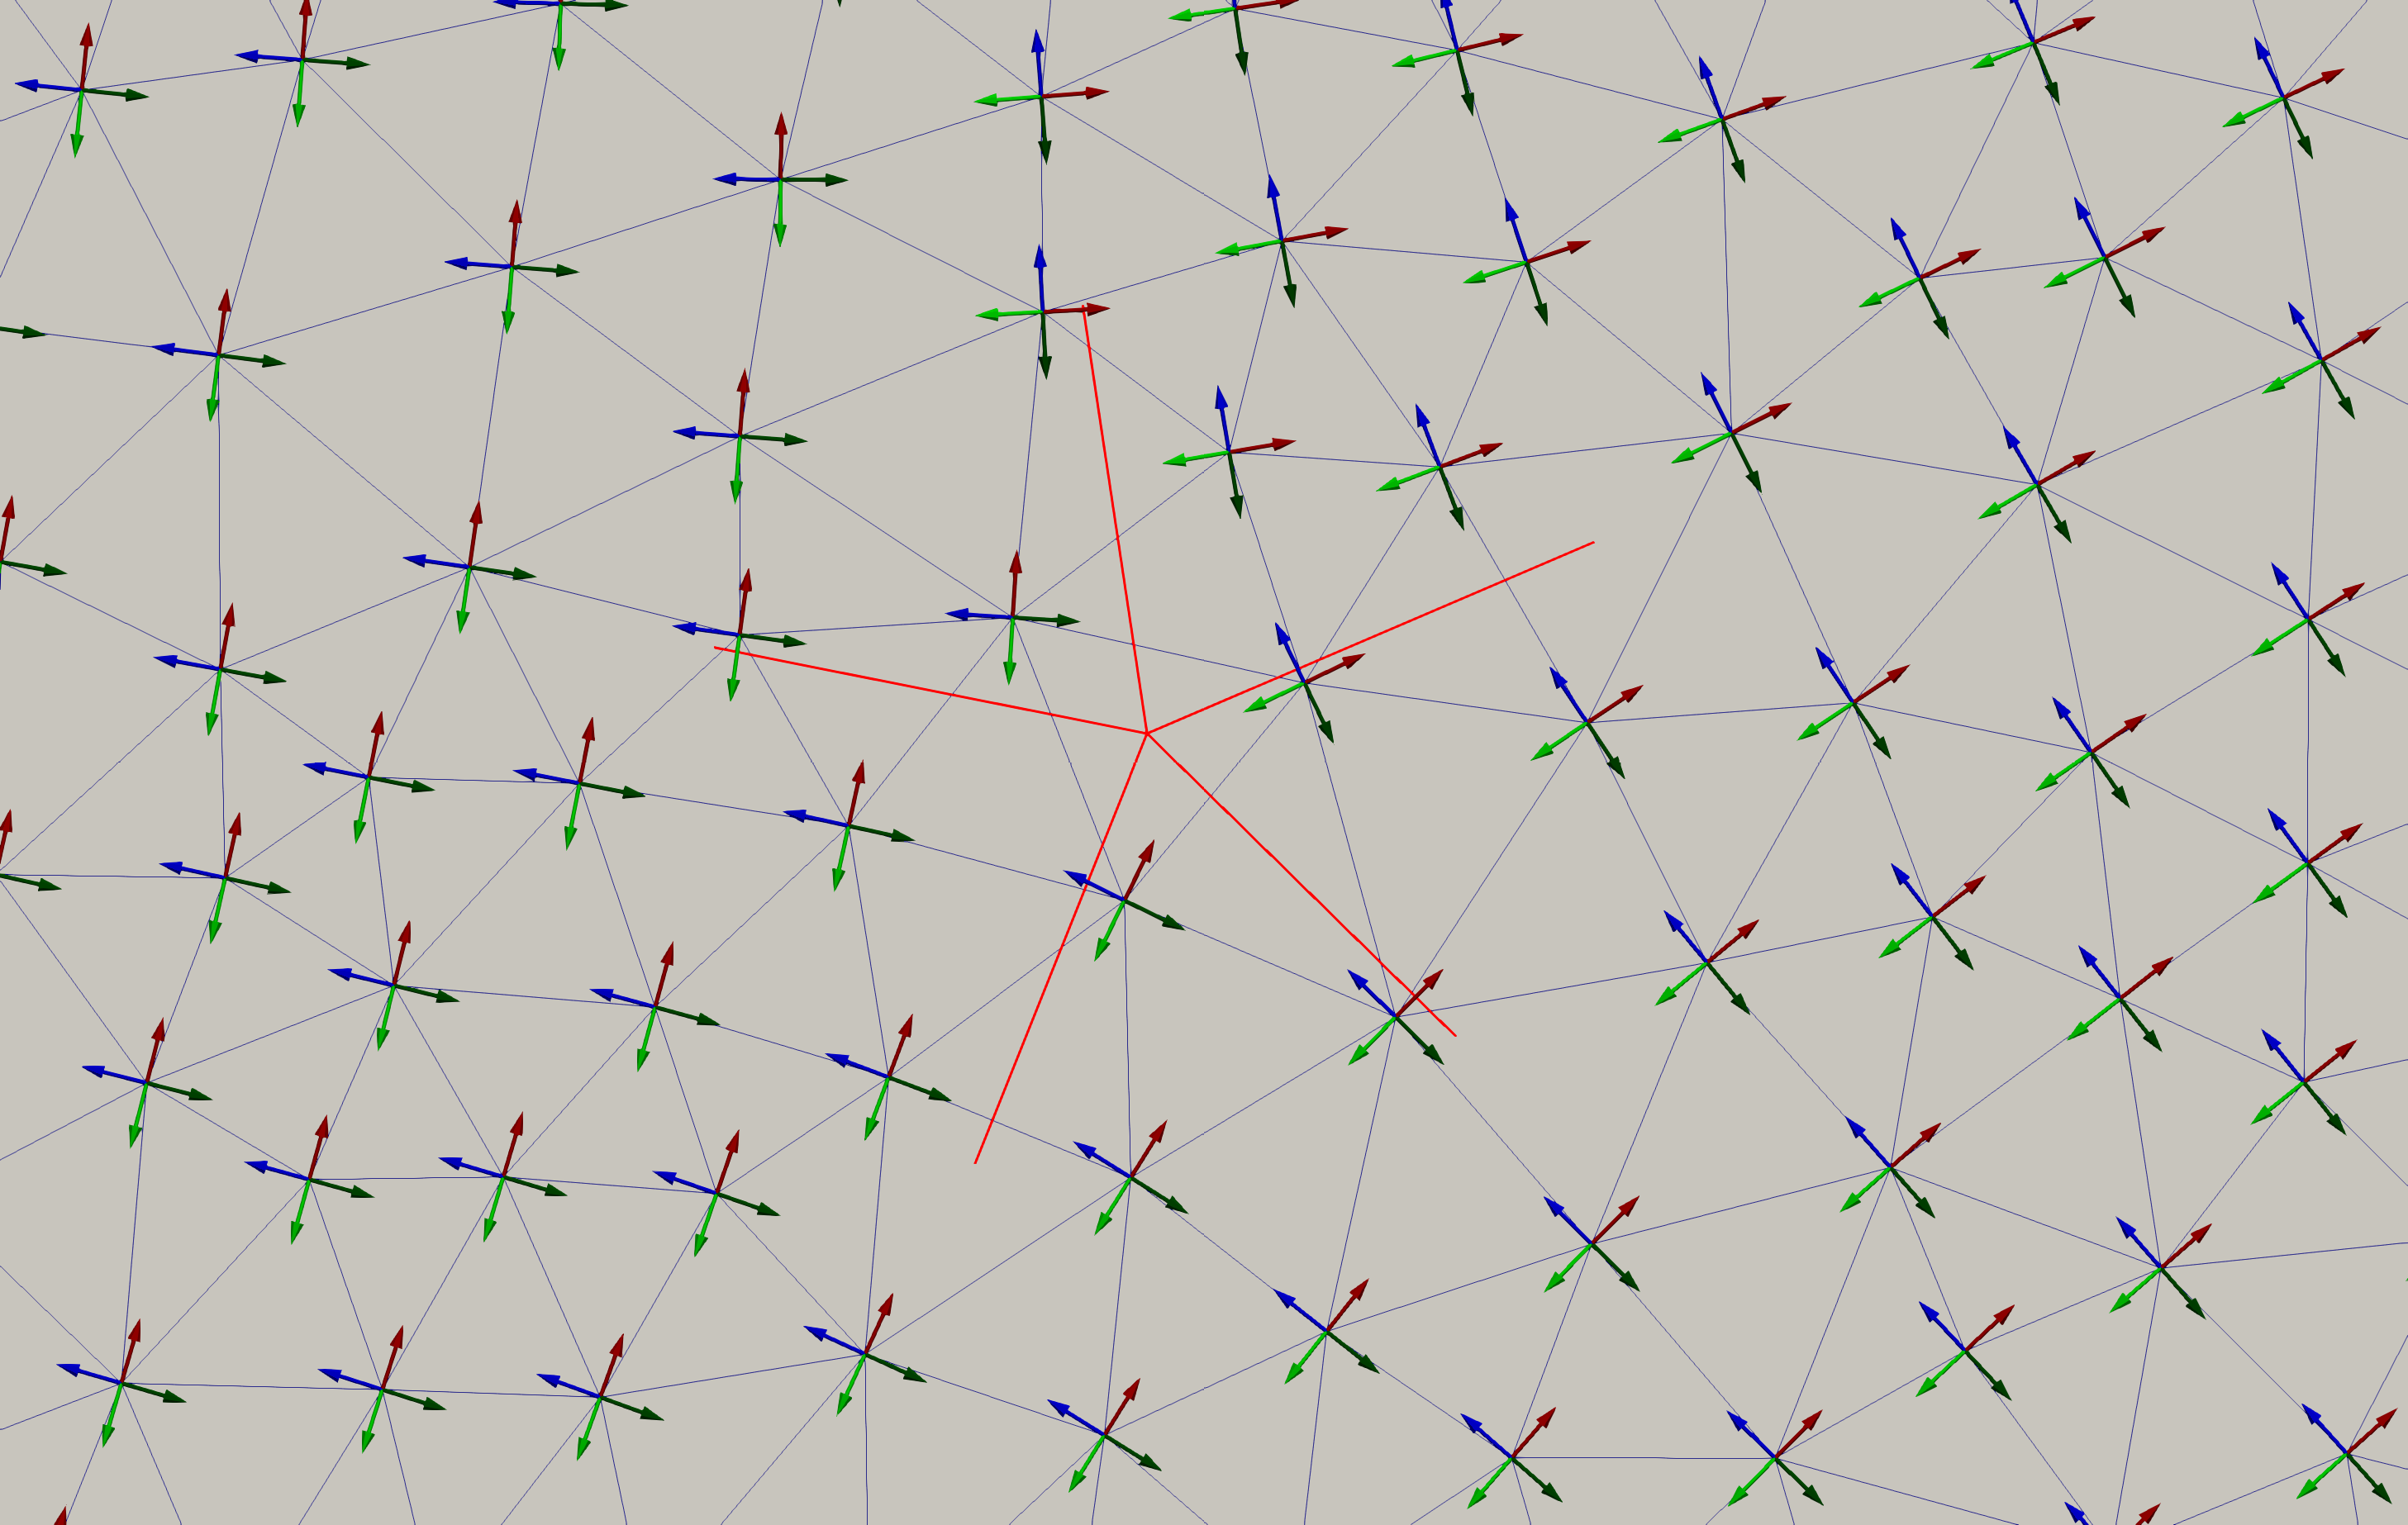
\includegraphics[height=7cm]{img/HIS-Slots-close-up.png}
		\end{itemize}
	}
	
	%%%%%%%%%%%%%%%%%%%%%%%%%%%%%%%%%%%%%%%%%%%%%%%%%%%%%%%%%%%%%%%%%%%%%%%%%%%%%%%%%%%%%%%%
	\frame {
		\frametitle{Singularity Graph Building}		
		\framesubtitle{Algorithm Steps}
		%\[\frac{-b \pm \sqrt{b^2 - c}}{2a}\]
		\ \center{A. Sequential Strategy}
		\begin{itemize}
			\item 1. (Iteratively) Depart from each singular point along each slot direction until
			\begin{itemize}
			\item a) reach boundary
			\item b) reach the confusing ball of a different singularity
			\end{itemize}
			\item 2. If line-line intersection $\Longrightarrow$ treat intersection point as singularity point for the patch layout construction
			
		\end{itemize}
	}
	
	%%%%%%%%%%%%%%%%%%%%%%%%%%%%%%%%%%%%%%%%%%%%%%%%%%%%%%%%%%%%%%%%%%%%%%%%%%%%%%%%%%%%%%%%
		\frame {
		\frametitle{Singularity Graph Building}		
		\framesubtitle{Algorithm Problems}
		%\[\frac{-b \pm \sqrt{b^2 - c}}{2a}\]
		\ \center{A. Sequential Strategy}
		\newline
		Difficulty in choosing the confusing ball radius;
		\newline 	
		If too small $\Longrightarrow$ singularities connected to boundary too often
	\begin{figure}[]
        \center{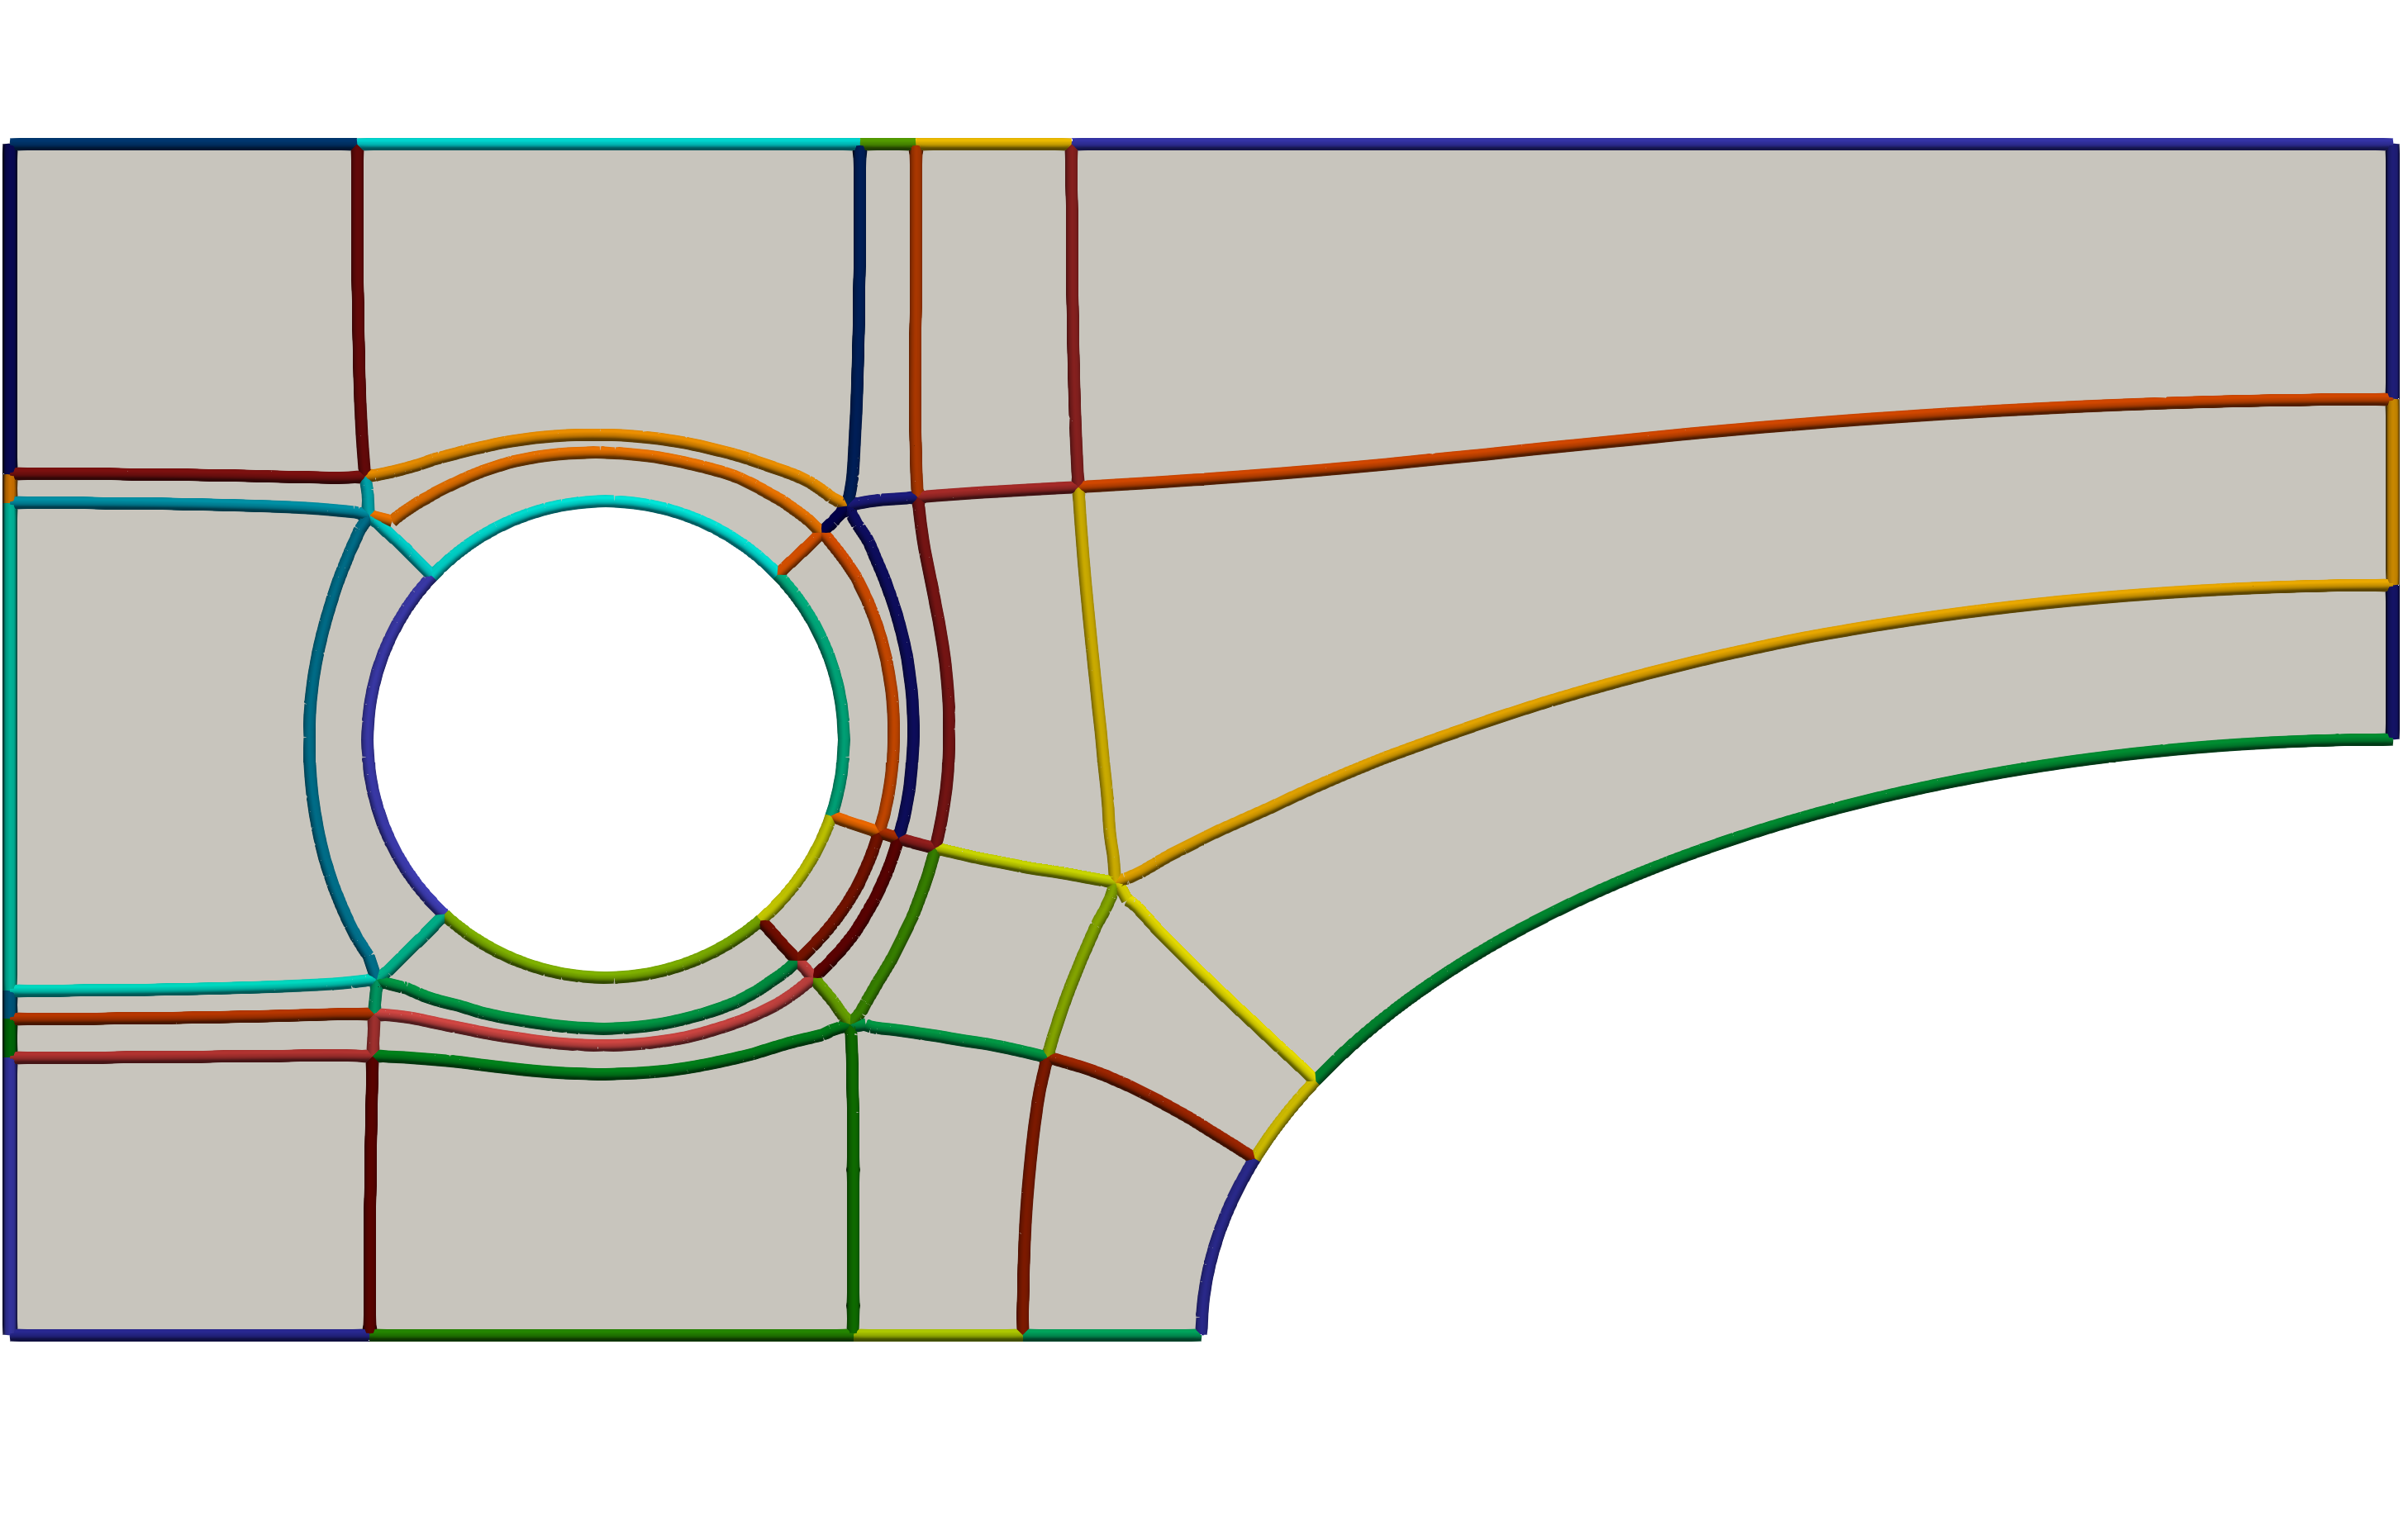
\includegraphics[width=8cm]
        {img/HIS-SingGraphOriginal-ConfusBallRad001.png}}
        \caption{ Mesh HIS - Singularity Graph - small confusing ball radius}
      \end{figure}		
		%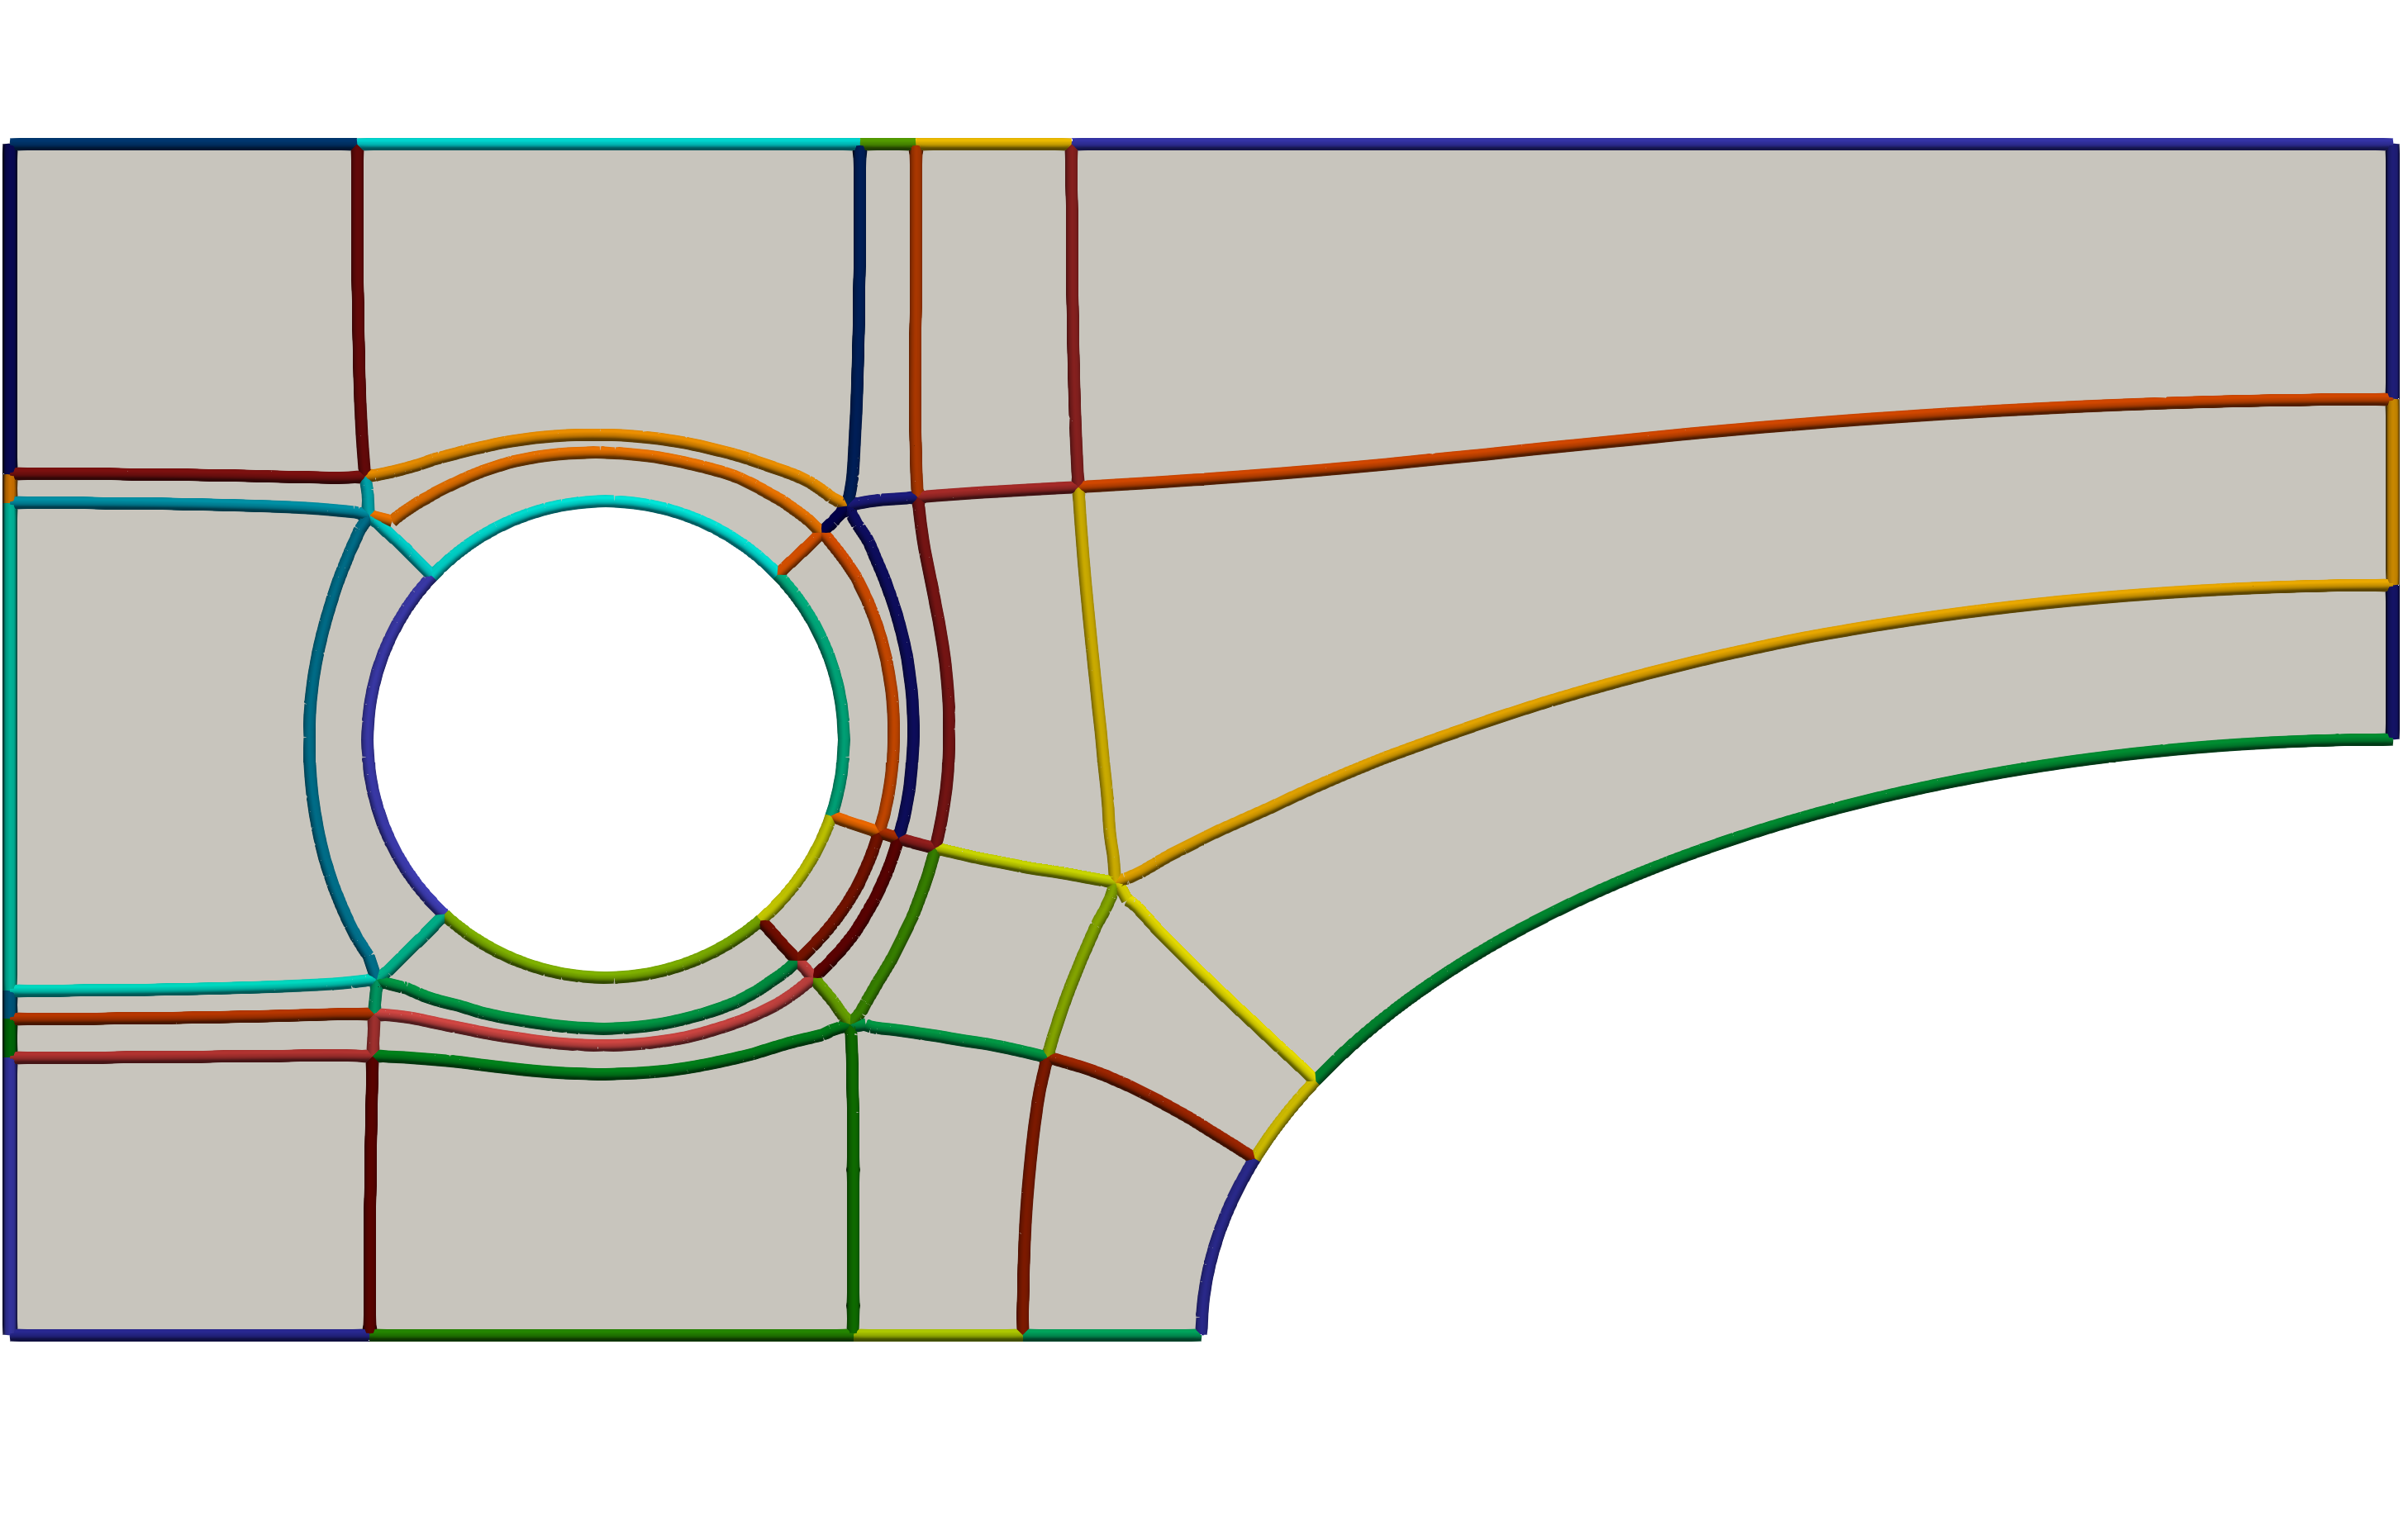
\includegraphics[height=7cm]{img/HIS-SingGraphOriginal-ConfusBallRad001.png}		
			
	}
	%%%%%%%%%%%%%%%%%%%%%%%%%%%%%%%%%%%%%%%%%%%%%%%%%%%%%%%%%%%%%%%%%%%%%%%%%%%%%%%%%%%%%%%%
	\begin{comment}
	\frame {
		\frametitle{Singularity Graph Building}		
		\framesubtitle{Algorithm Problems}
		%\[\frac{-b \pm \sqrt{b^2 - c}}{2a}\]
		\ \center{A. Sequential Strategy}
		\begin{columns}[T] % contents are top vertically aligned
     	\begin{column}[T]{5cm} % each column can also be its own environment
     	
     	\begin{figure}[]
        \center{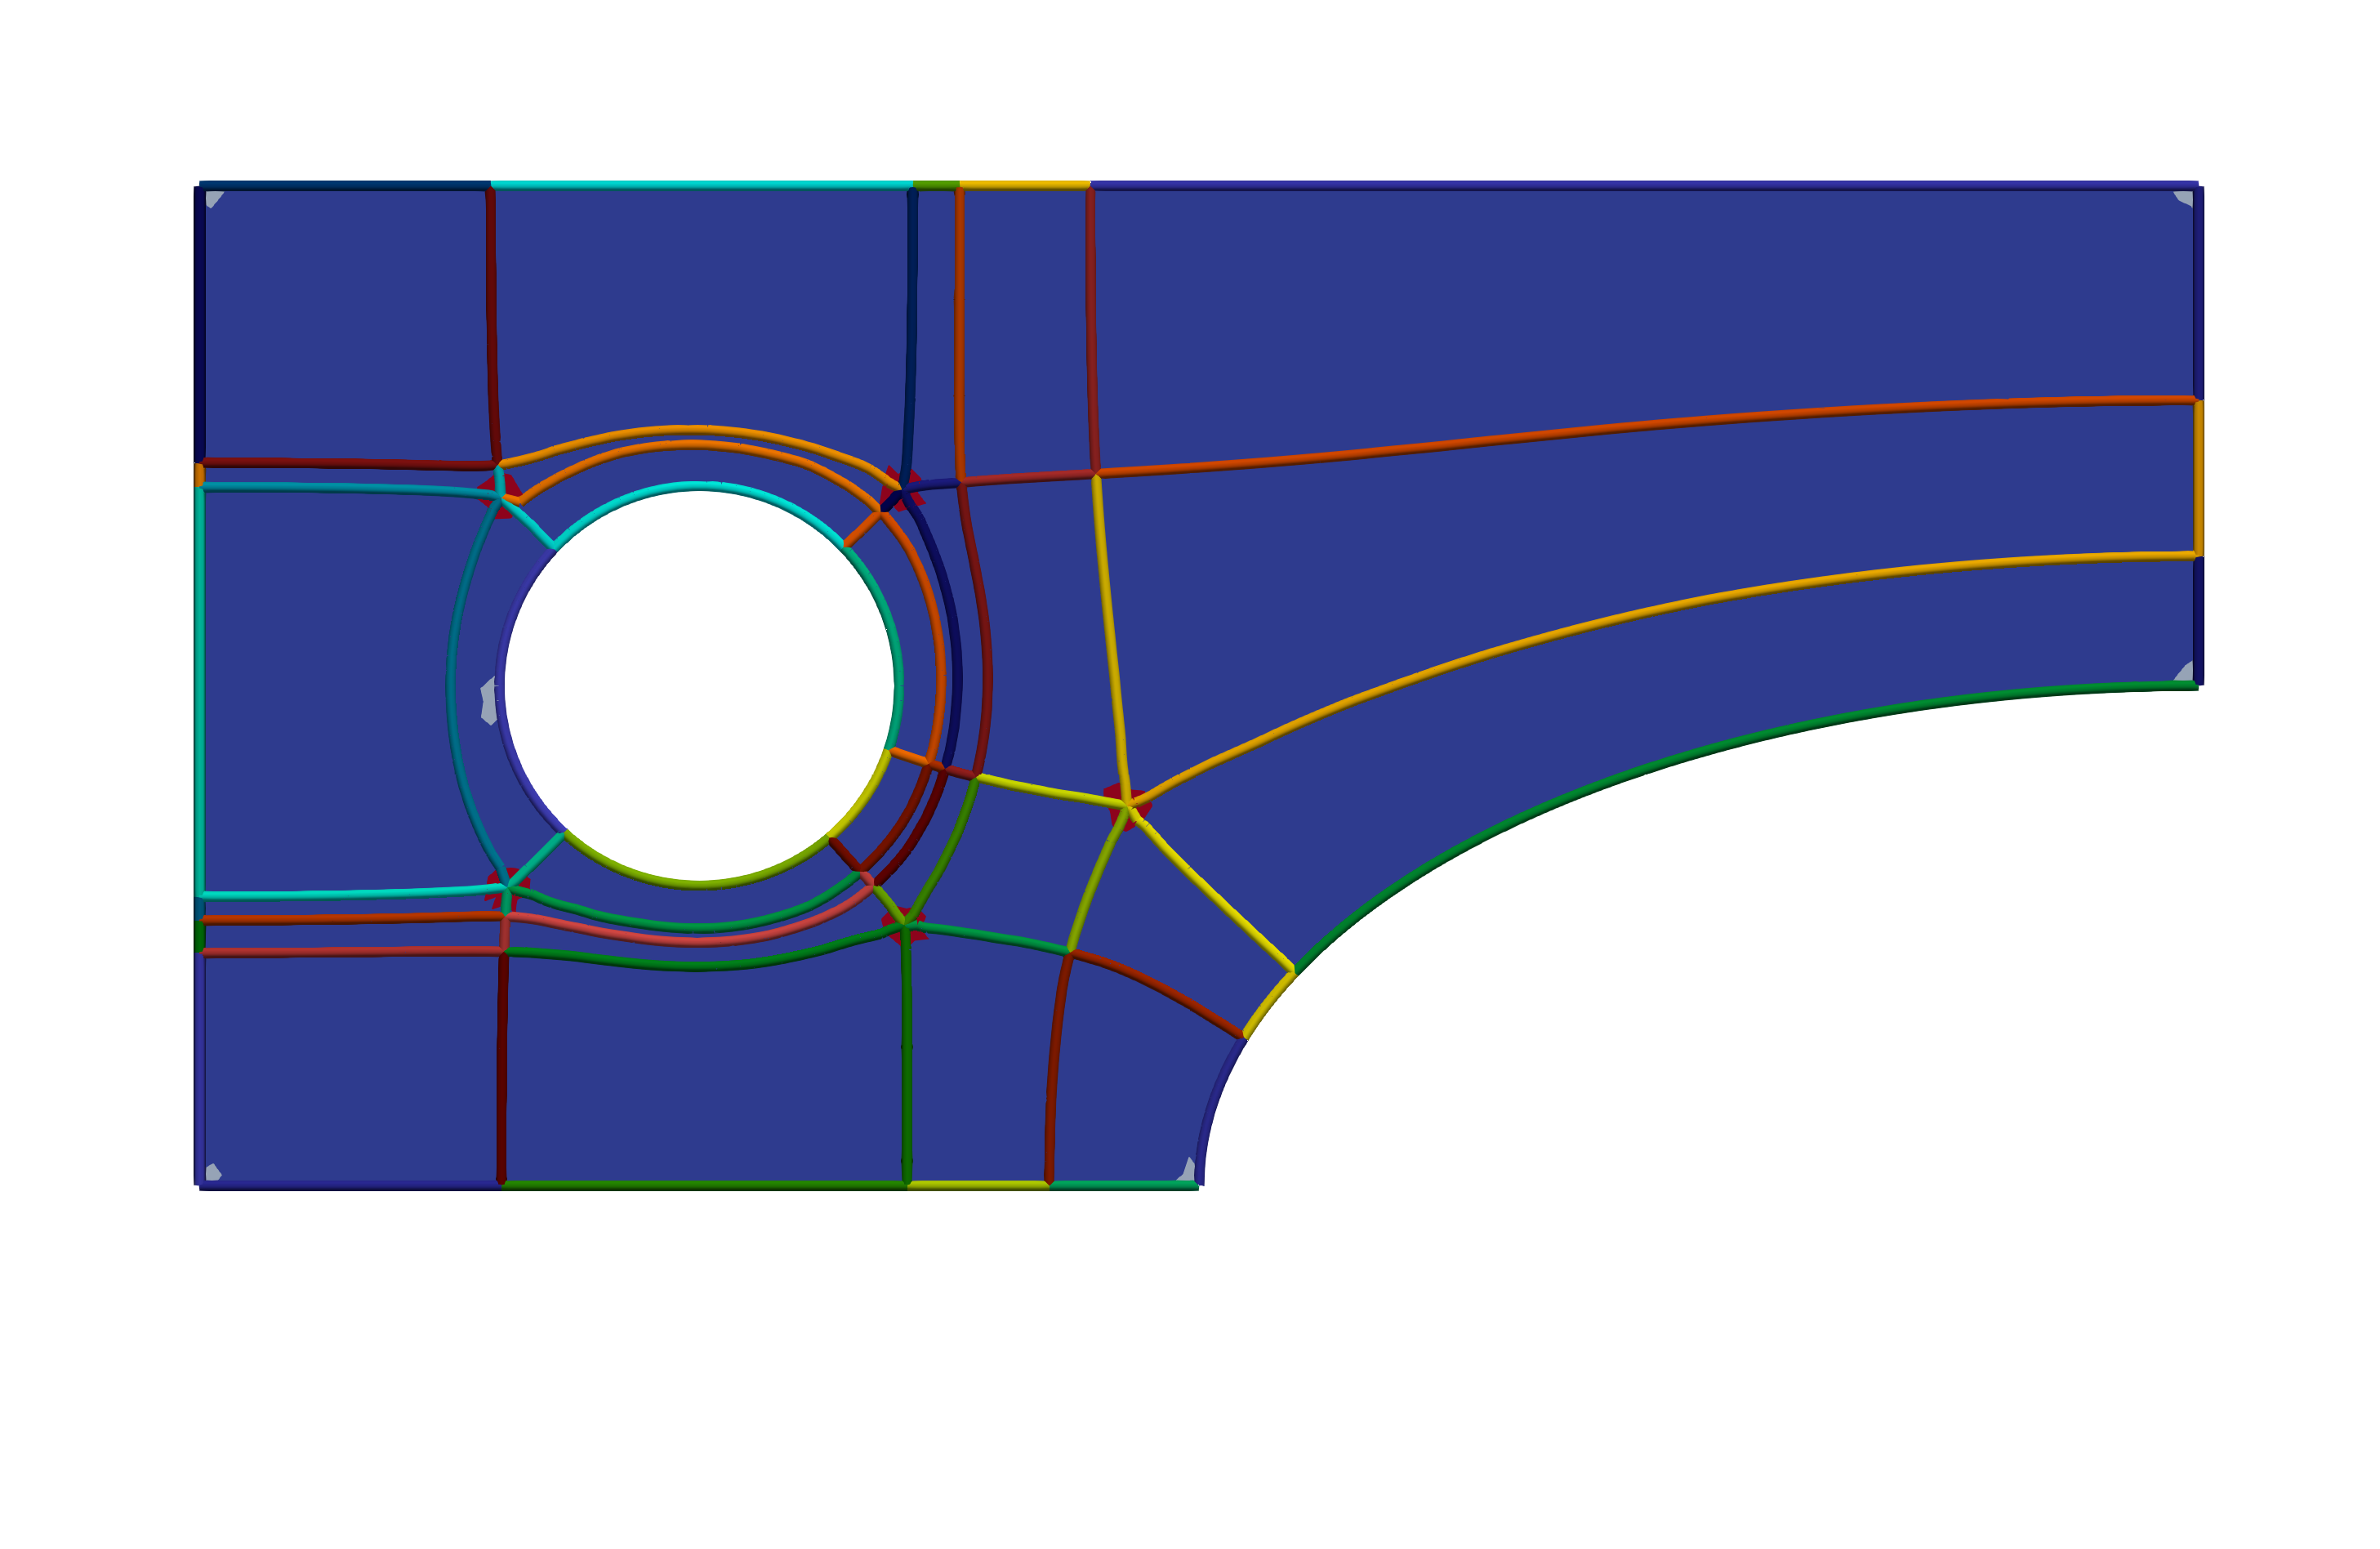
\includegraphics[width=5cm]
        {img/HIS-SingGraphOriginal-ConfusBallRad001confusBall.png}}
        \caption{ Normal Radius}
      \end{figure}	
     	%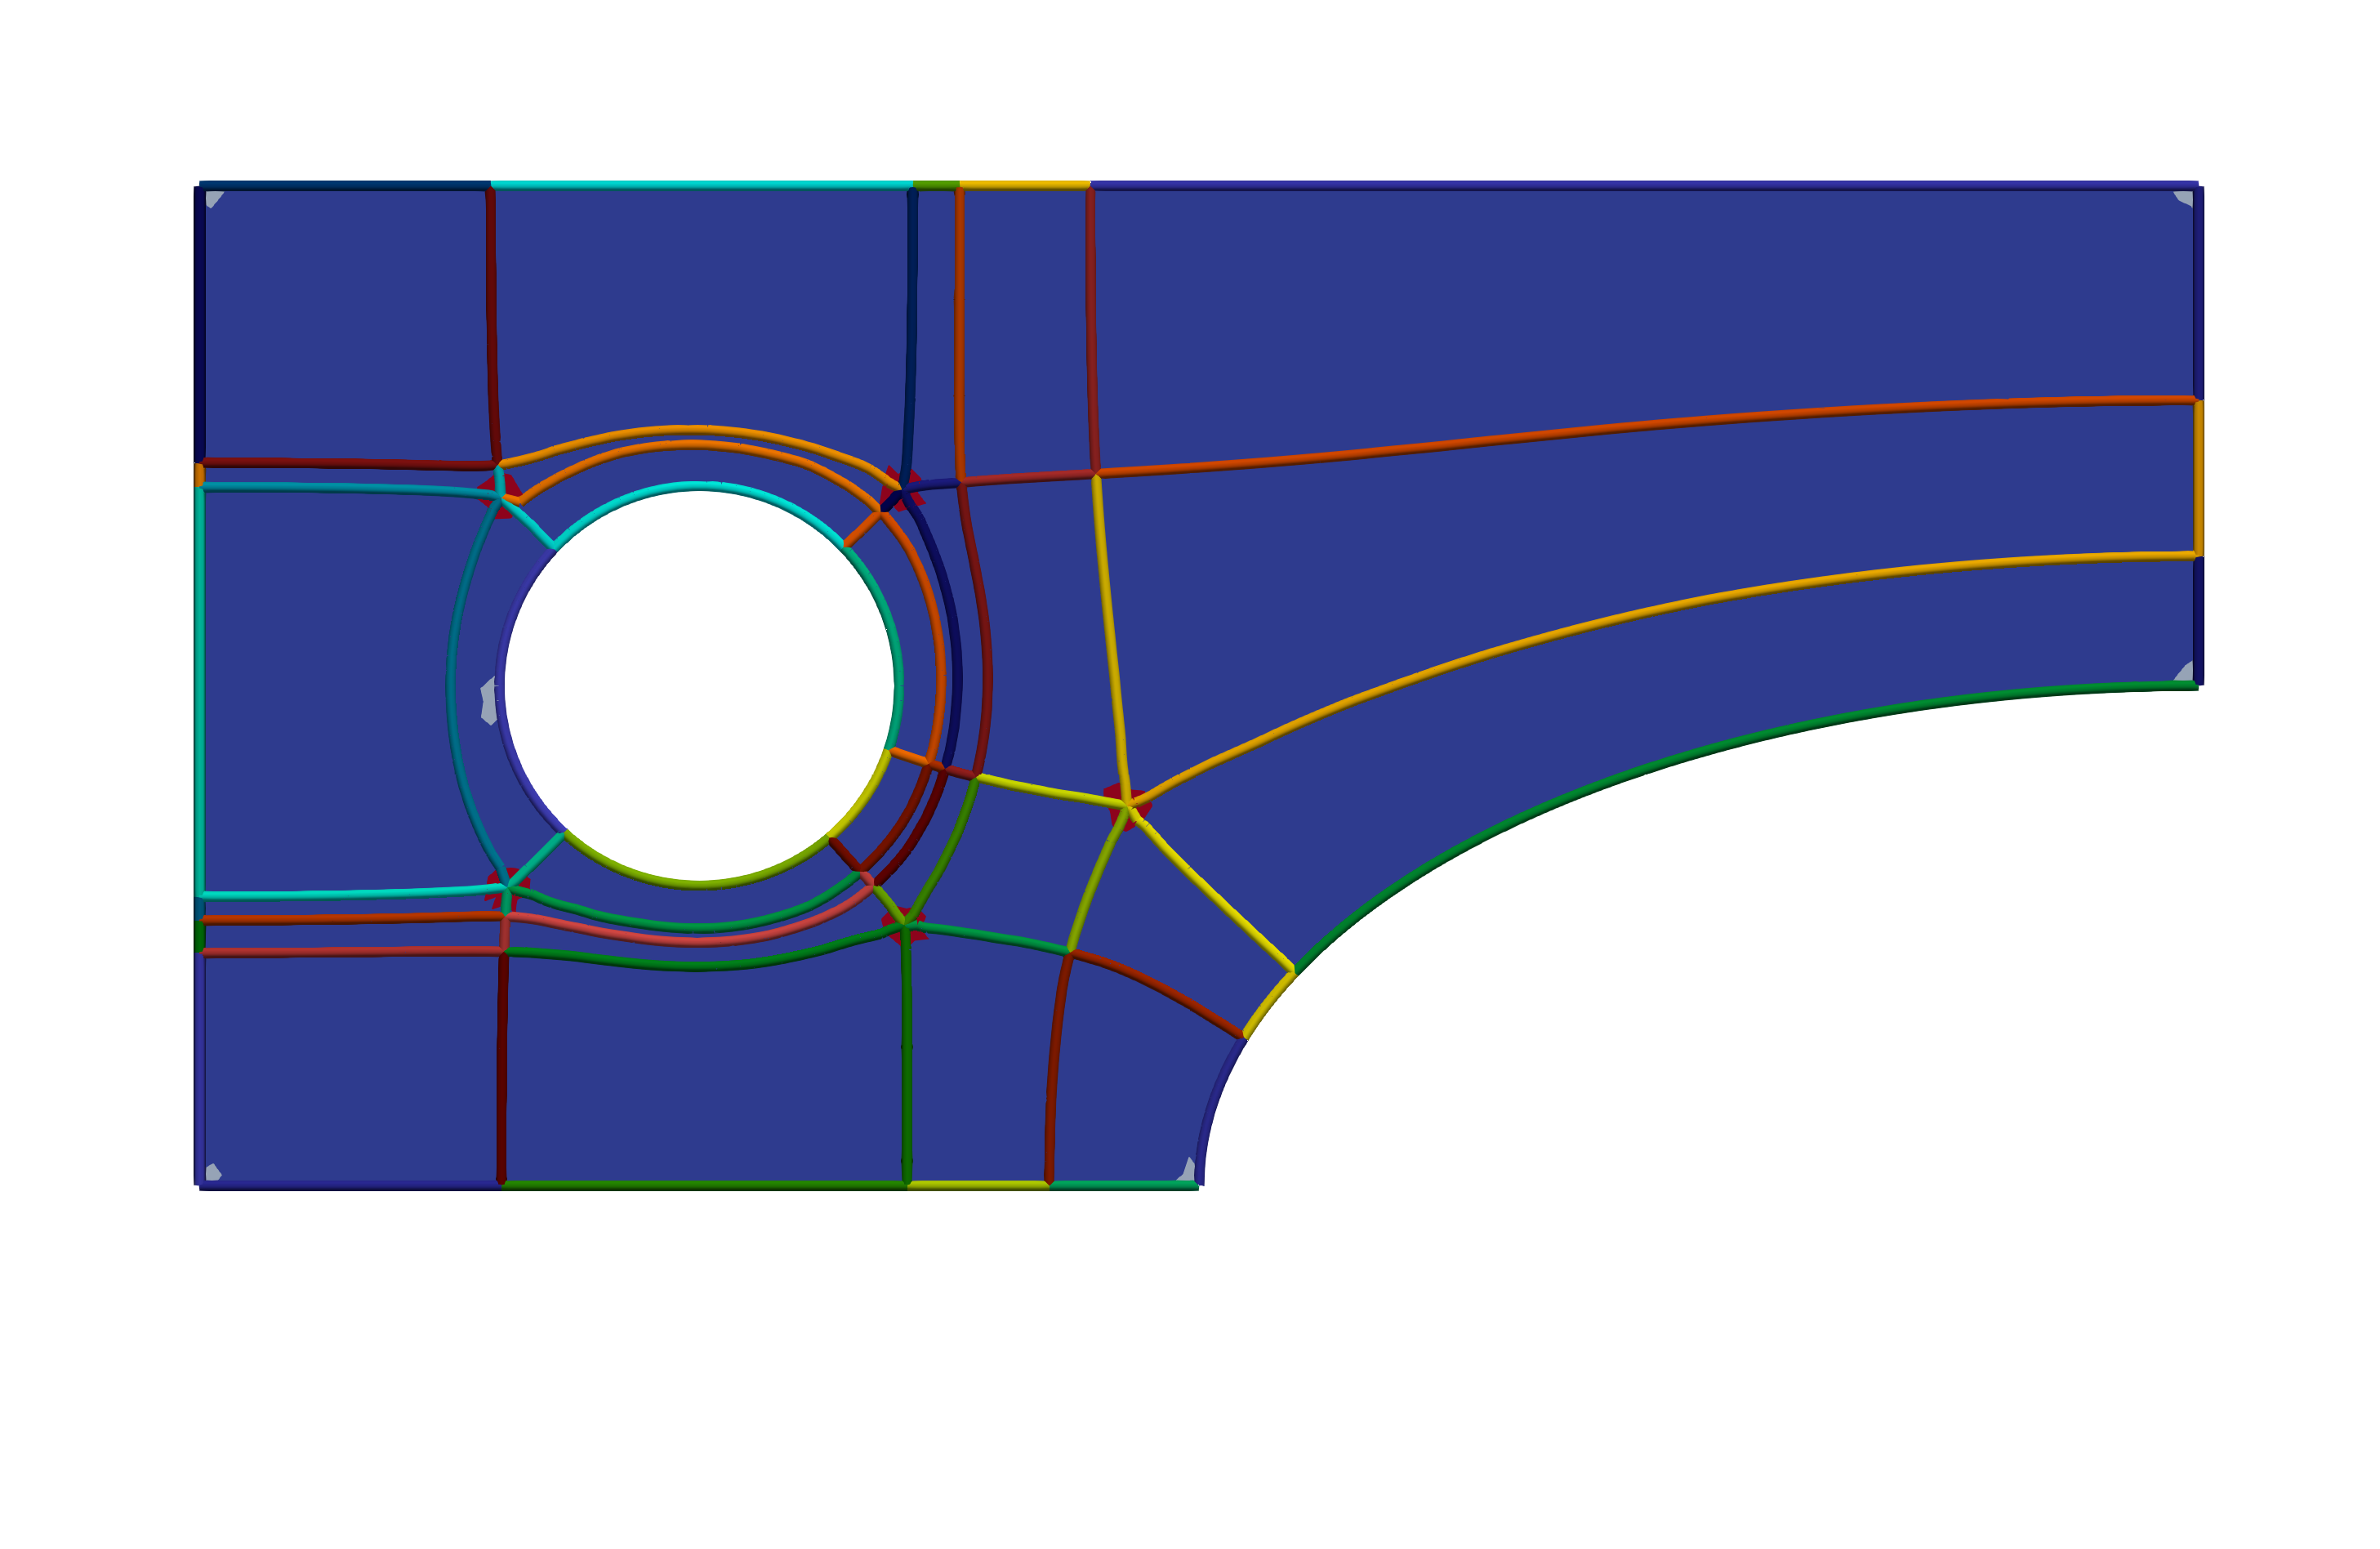
\includegraphics[height=3.7cm]{img/HIS-SingGraphOriginal-ConfusBallRad001confusBall.png}
     	\end{column}
     	\begin{column}[T]{5cm} % alternative top-align that's better for graphics
     	 
     	\begin{figure}[]
        \center{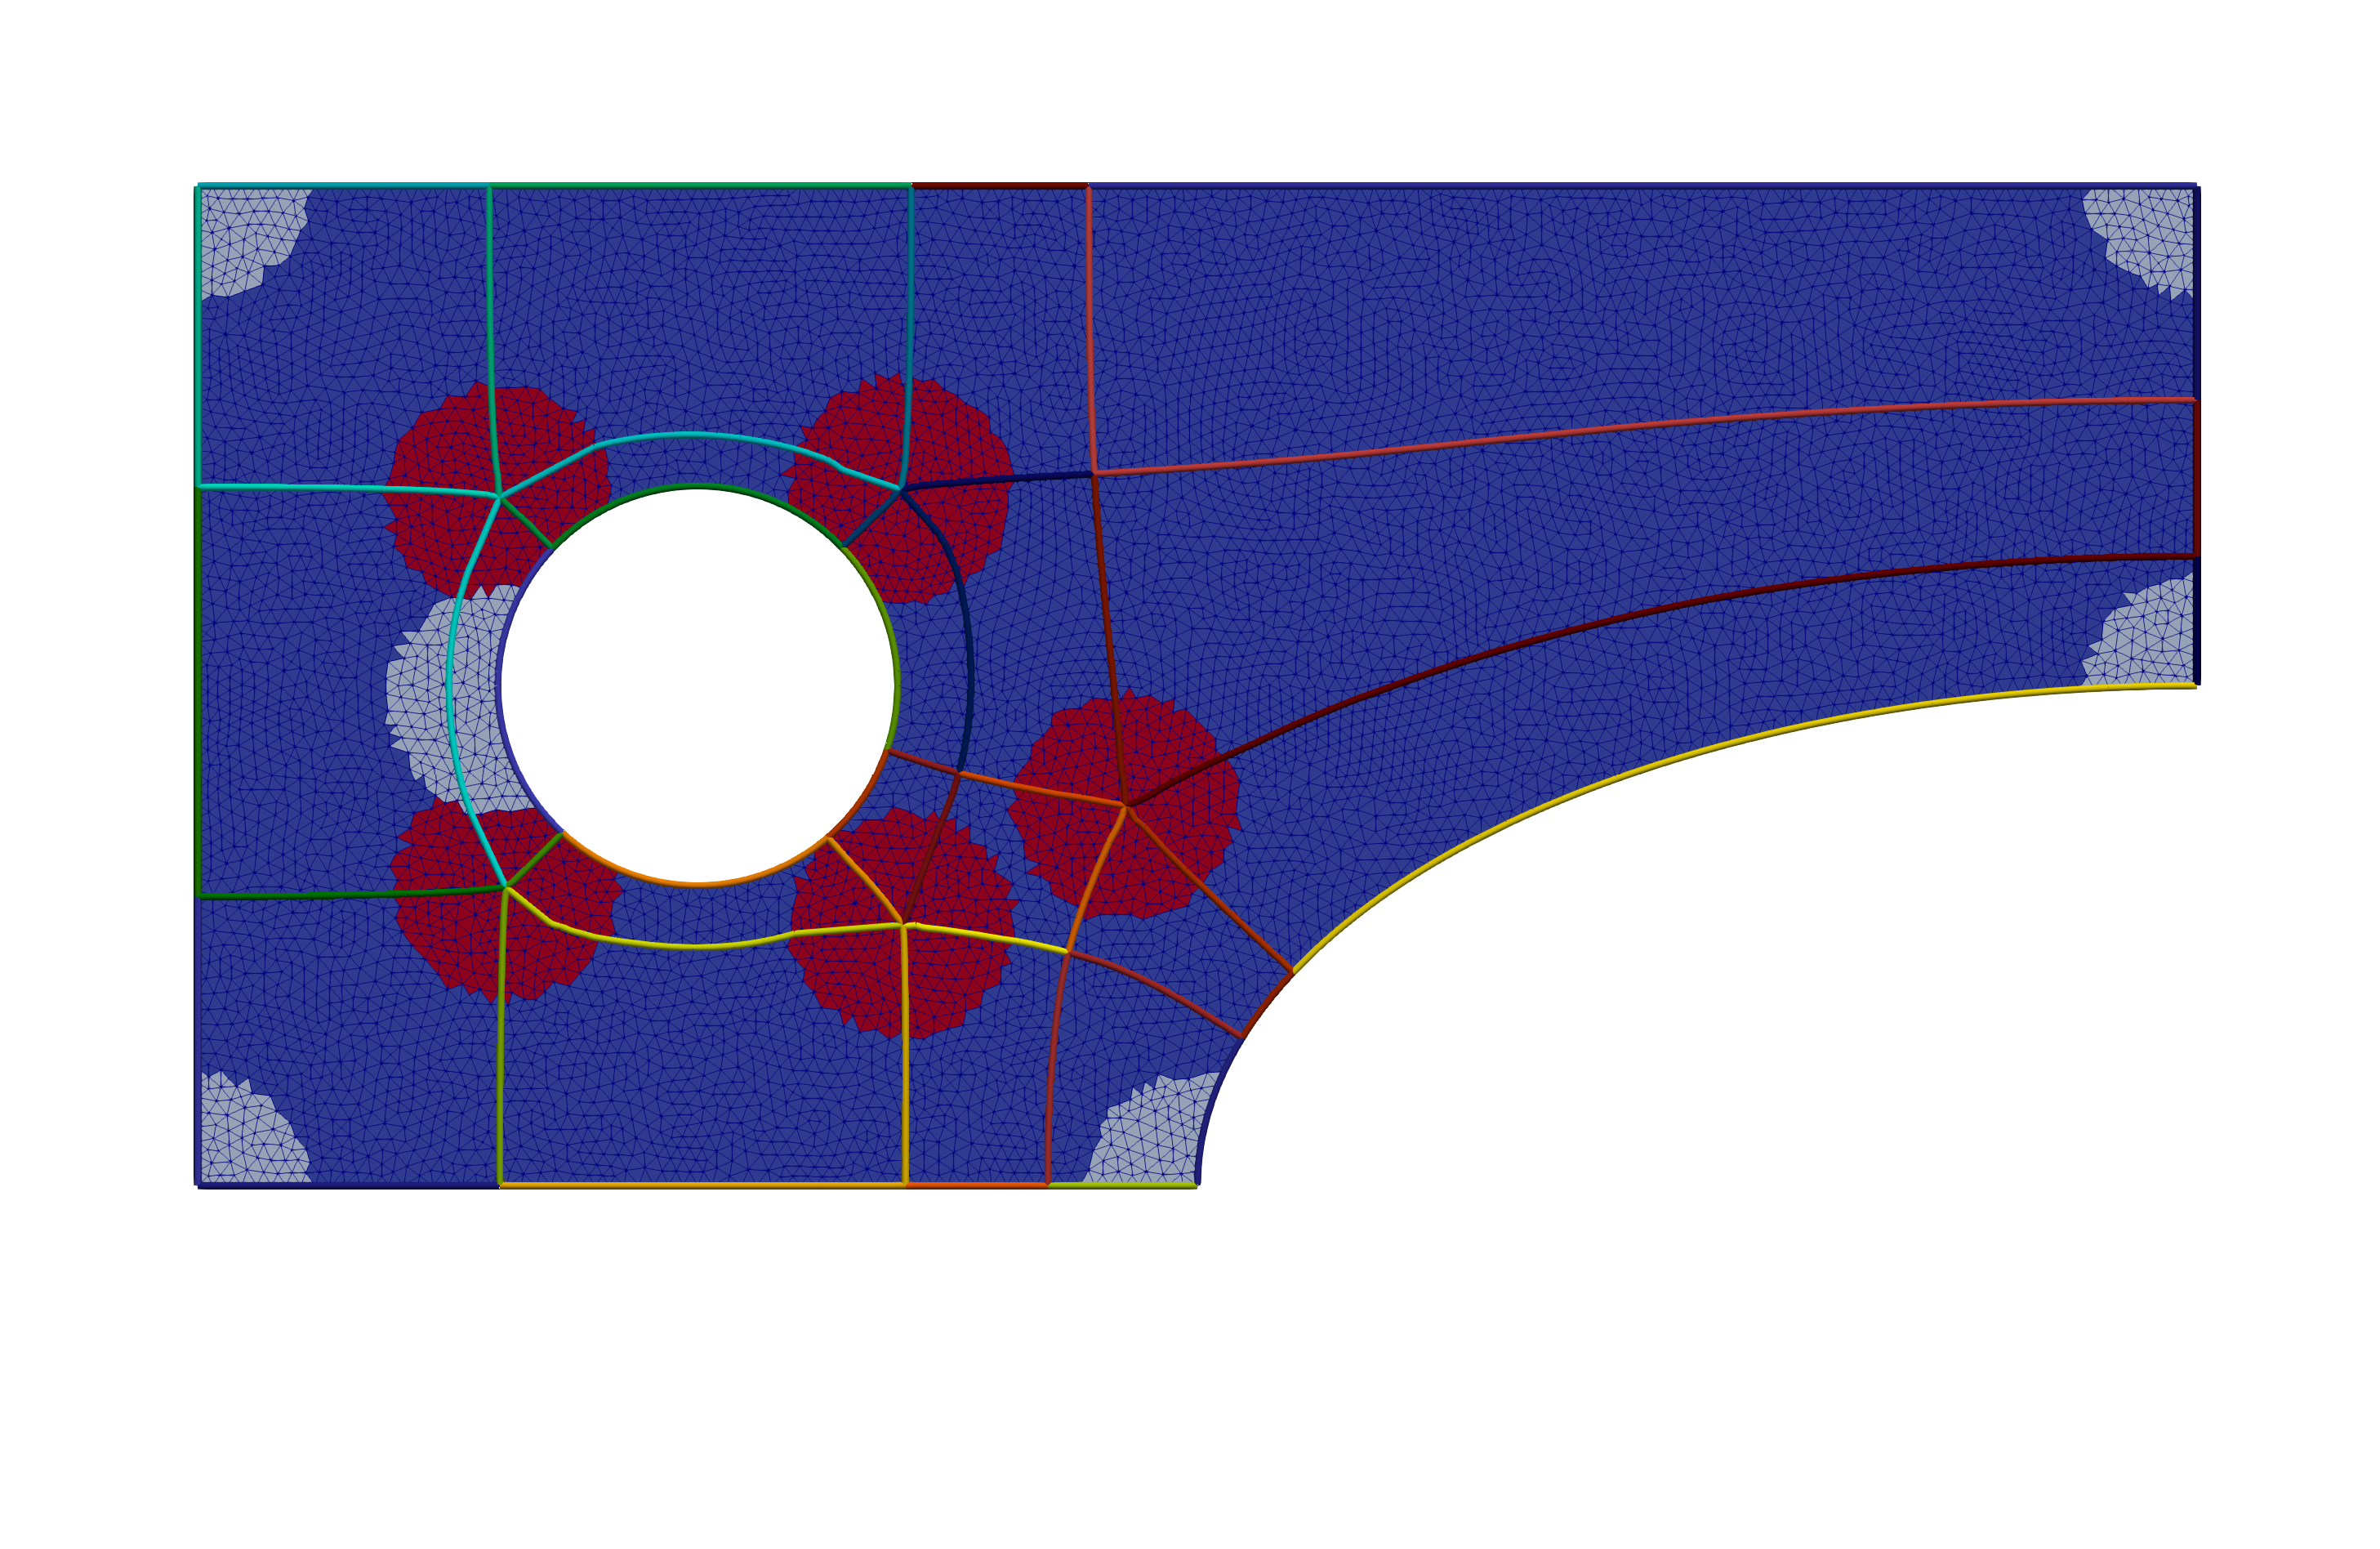
\includegraphics[width=5cm]
        {img/HIS-SingGraphOriginal-ConfusBallRad005confusBall.png}}
        \caption{ Big Radius}
      \end{figure}	
          %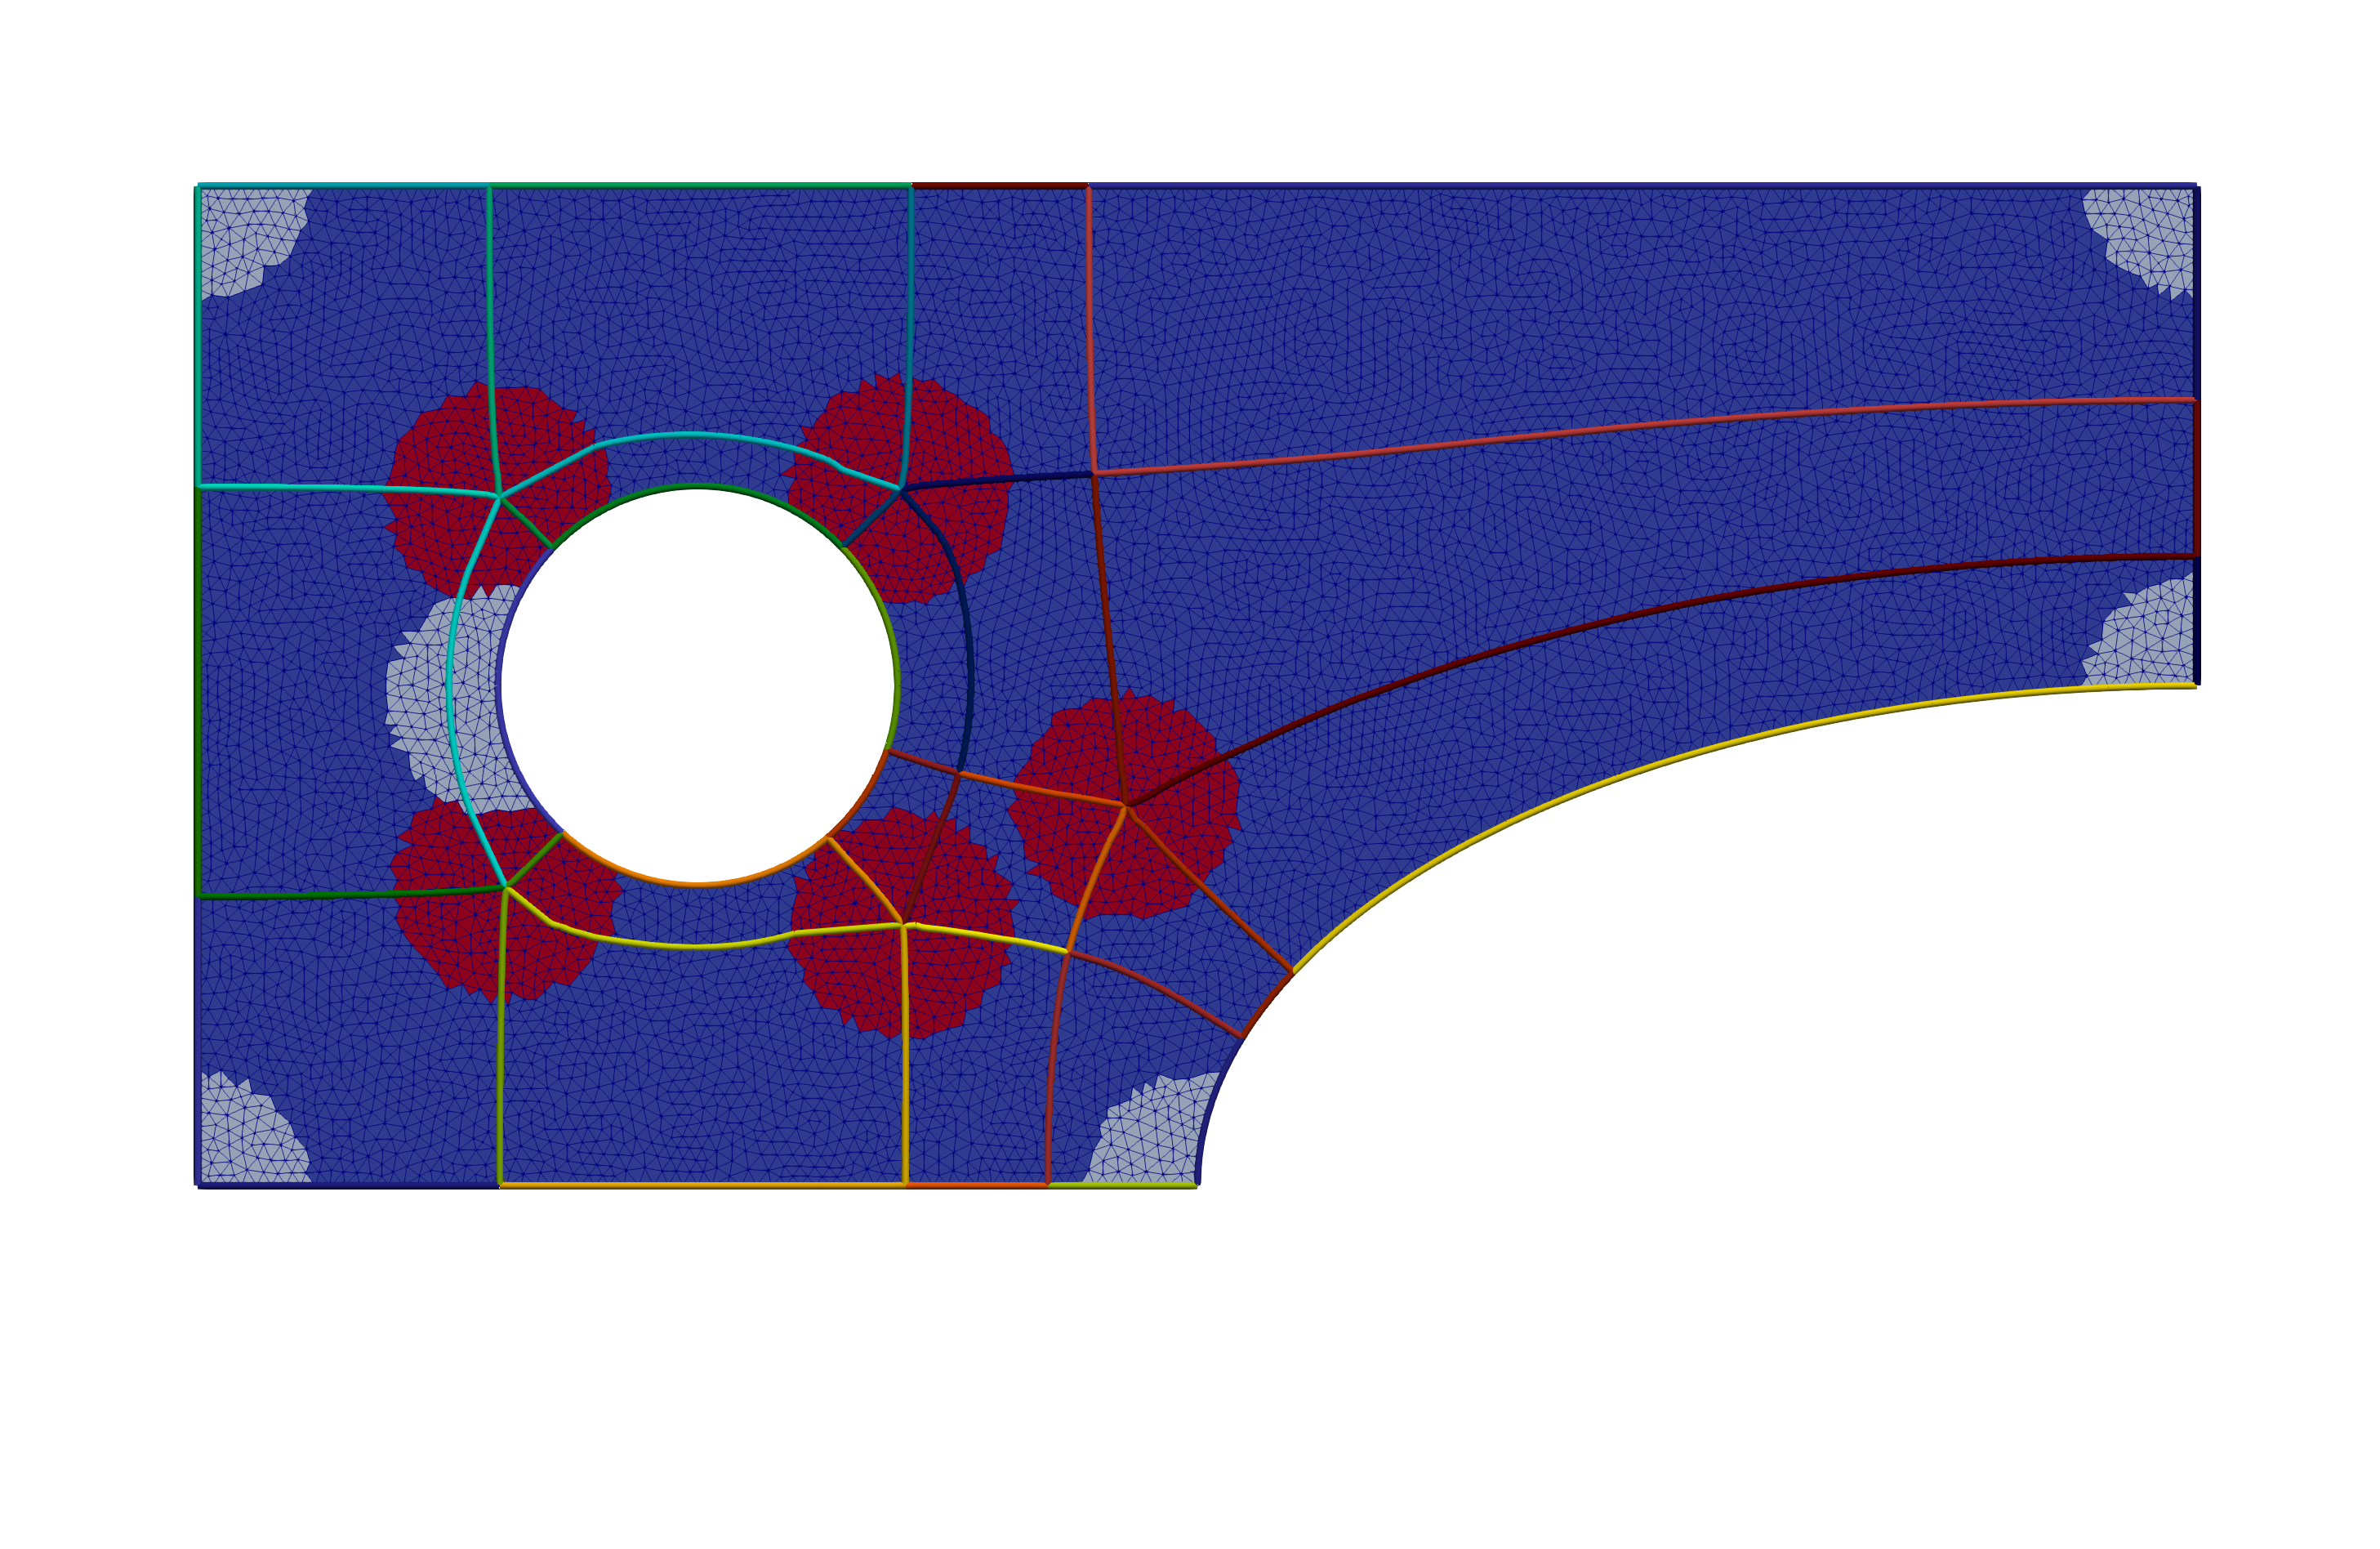
\includegraphics[height=3.7cm]{img/HIS-SingGraphOriginal-ConfusBallRad005confusBall.png}
     	\end{column}
     	\end{columns}
			
	}
	\end{comment}
	%%%%%%%%%%%%%%%%%%%%%%%%%%%%%%%%%%%%%%%%%%%%%%%%%%%%%%%%%%%%%%%%%%%%%%%%%%%%%%%%%%%%%%%%
	
	
	\frame {
		\frametitle{Singularity Graph Building}		
		\framesubtitle{Algorithm Problems}		
		\ \center{A. Sequential Strategy}
		
     	
     	\begin{figure}[]
     	\begin{subfigure}{\linewidth}
  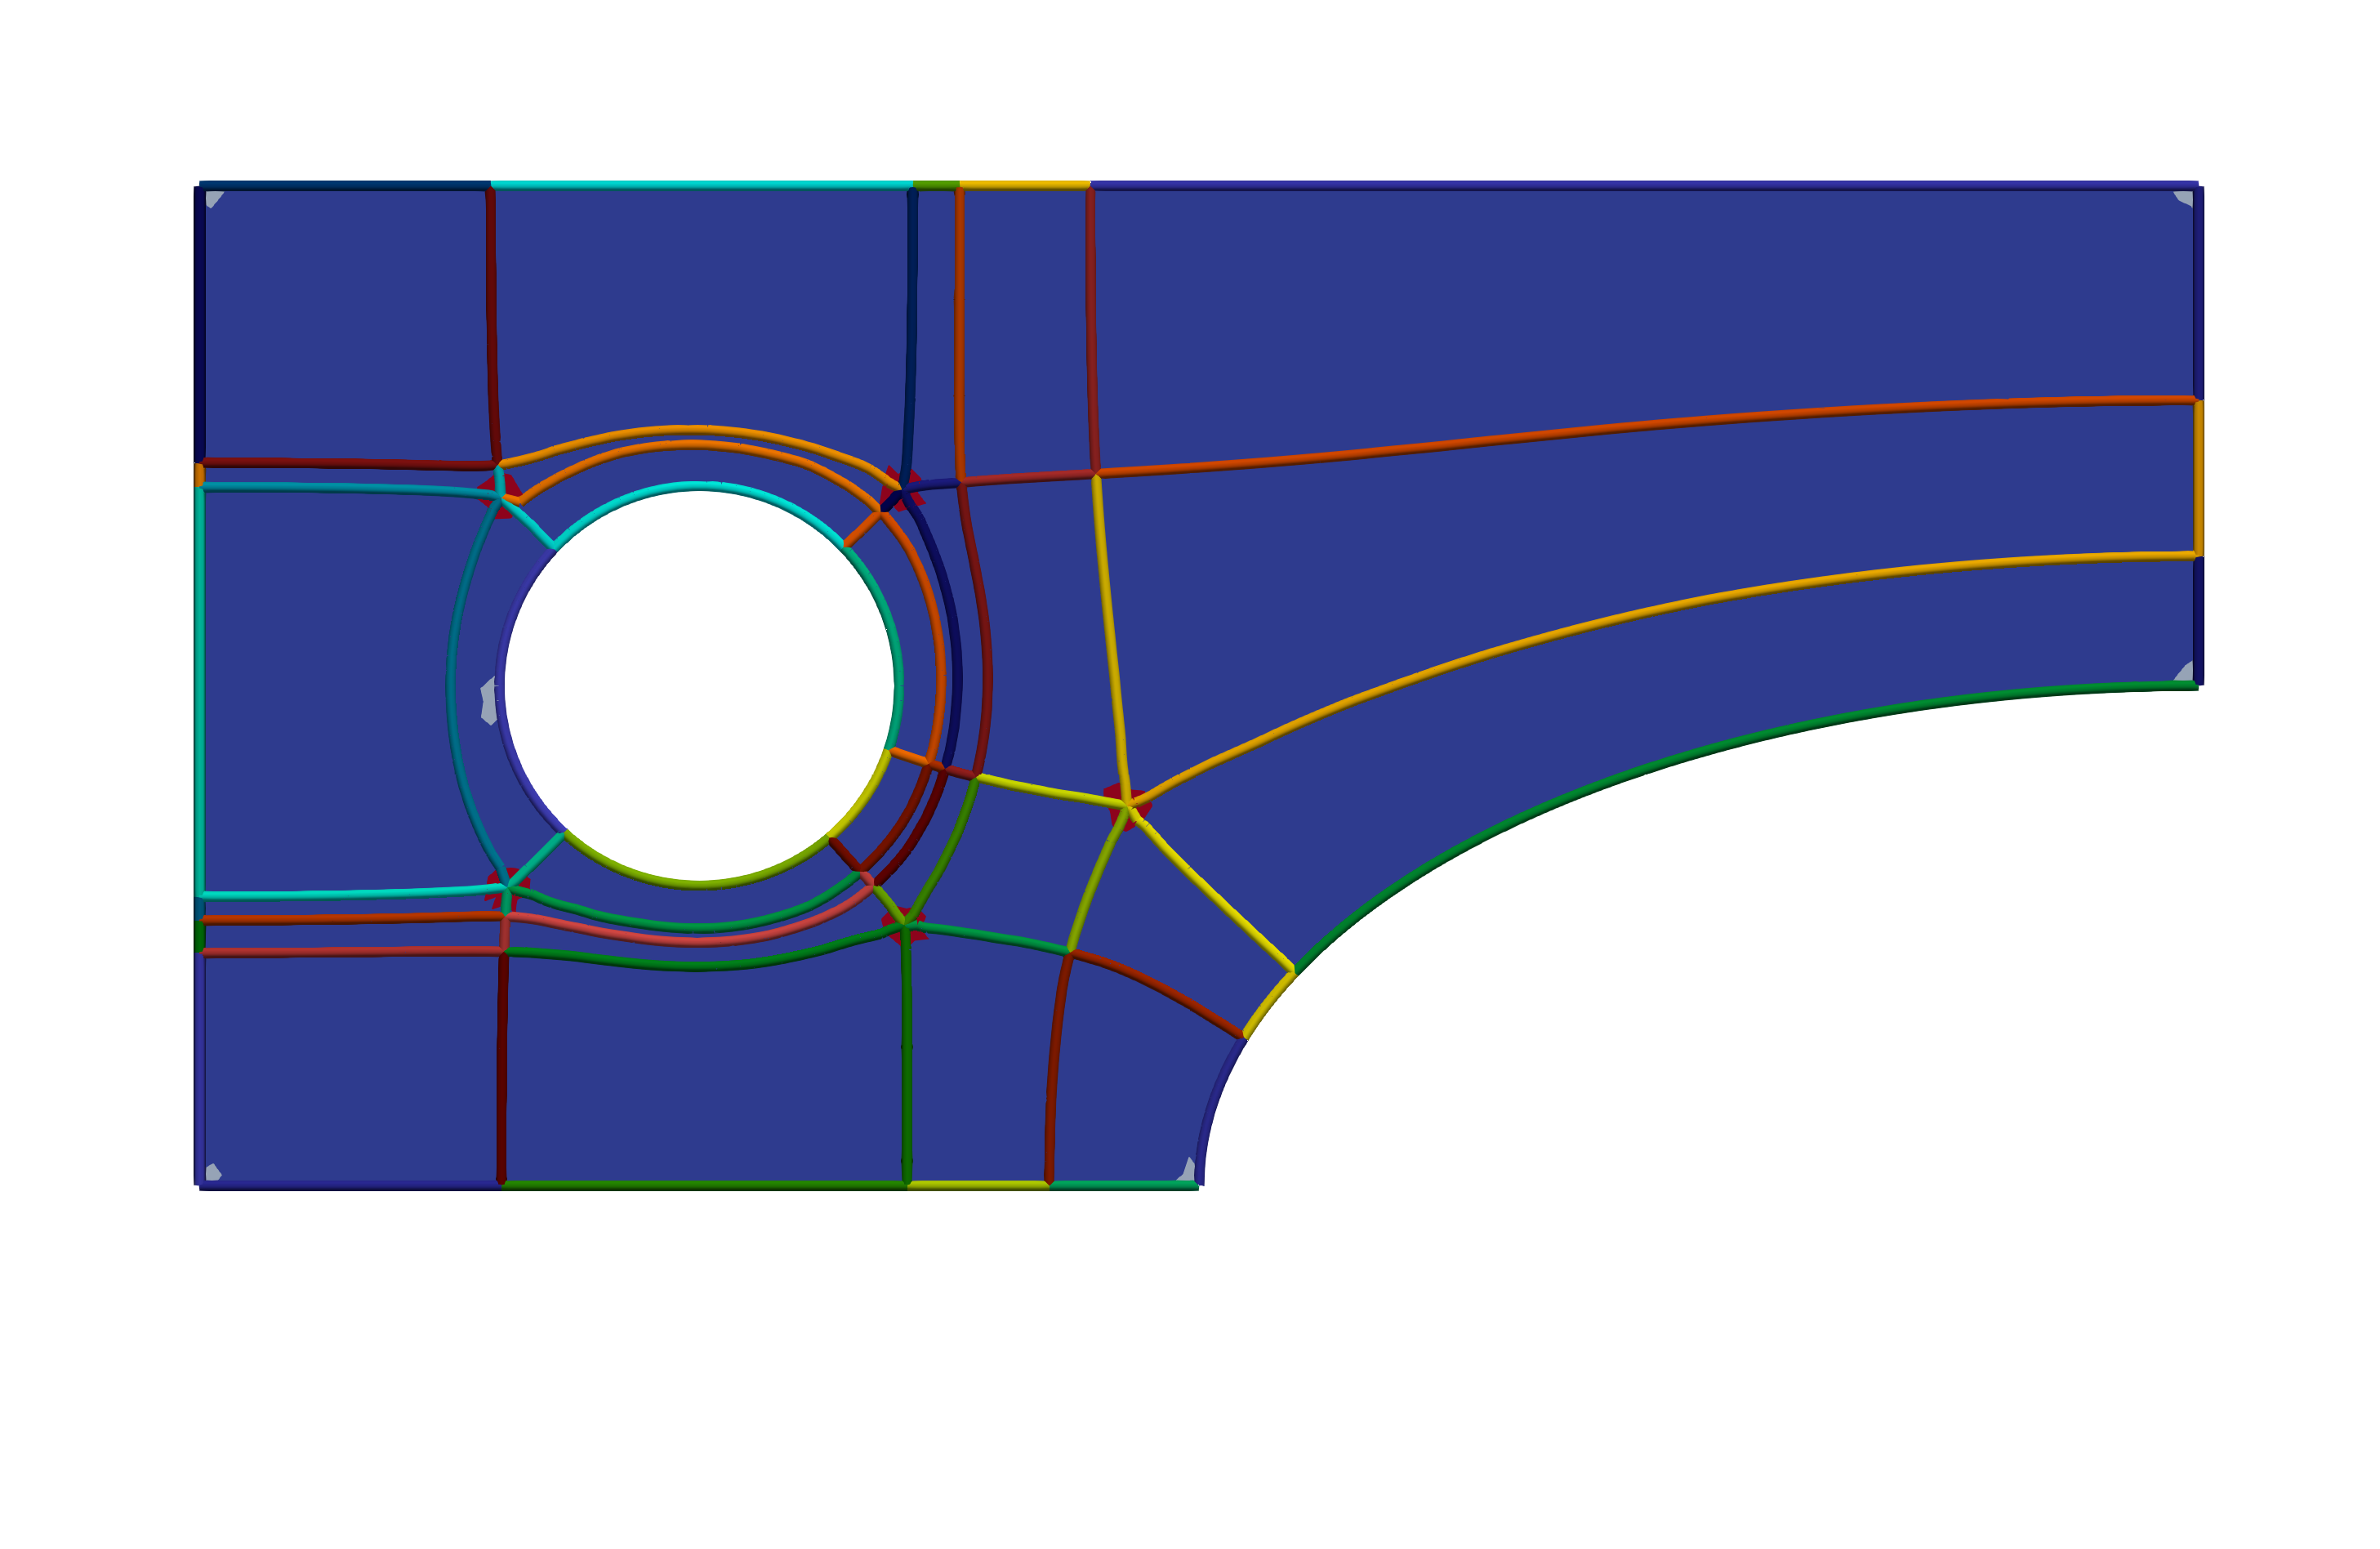
\includegraphics[width=.5\linewidth]
  {img/HIS-SingGraphOriginal-ConfusBallRad001confusBall.png}\hfill
  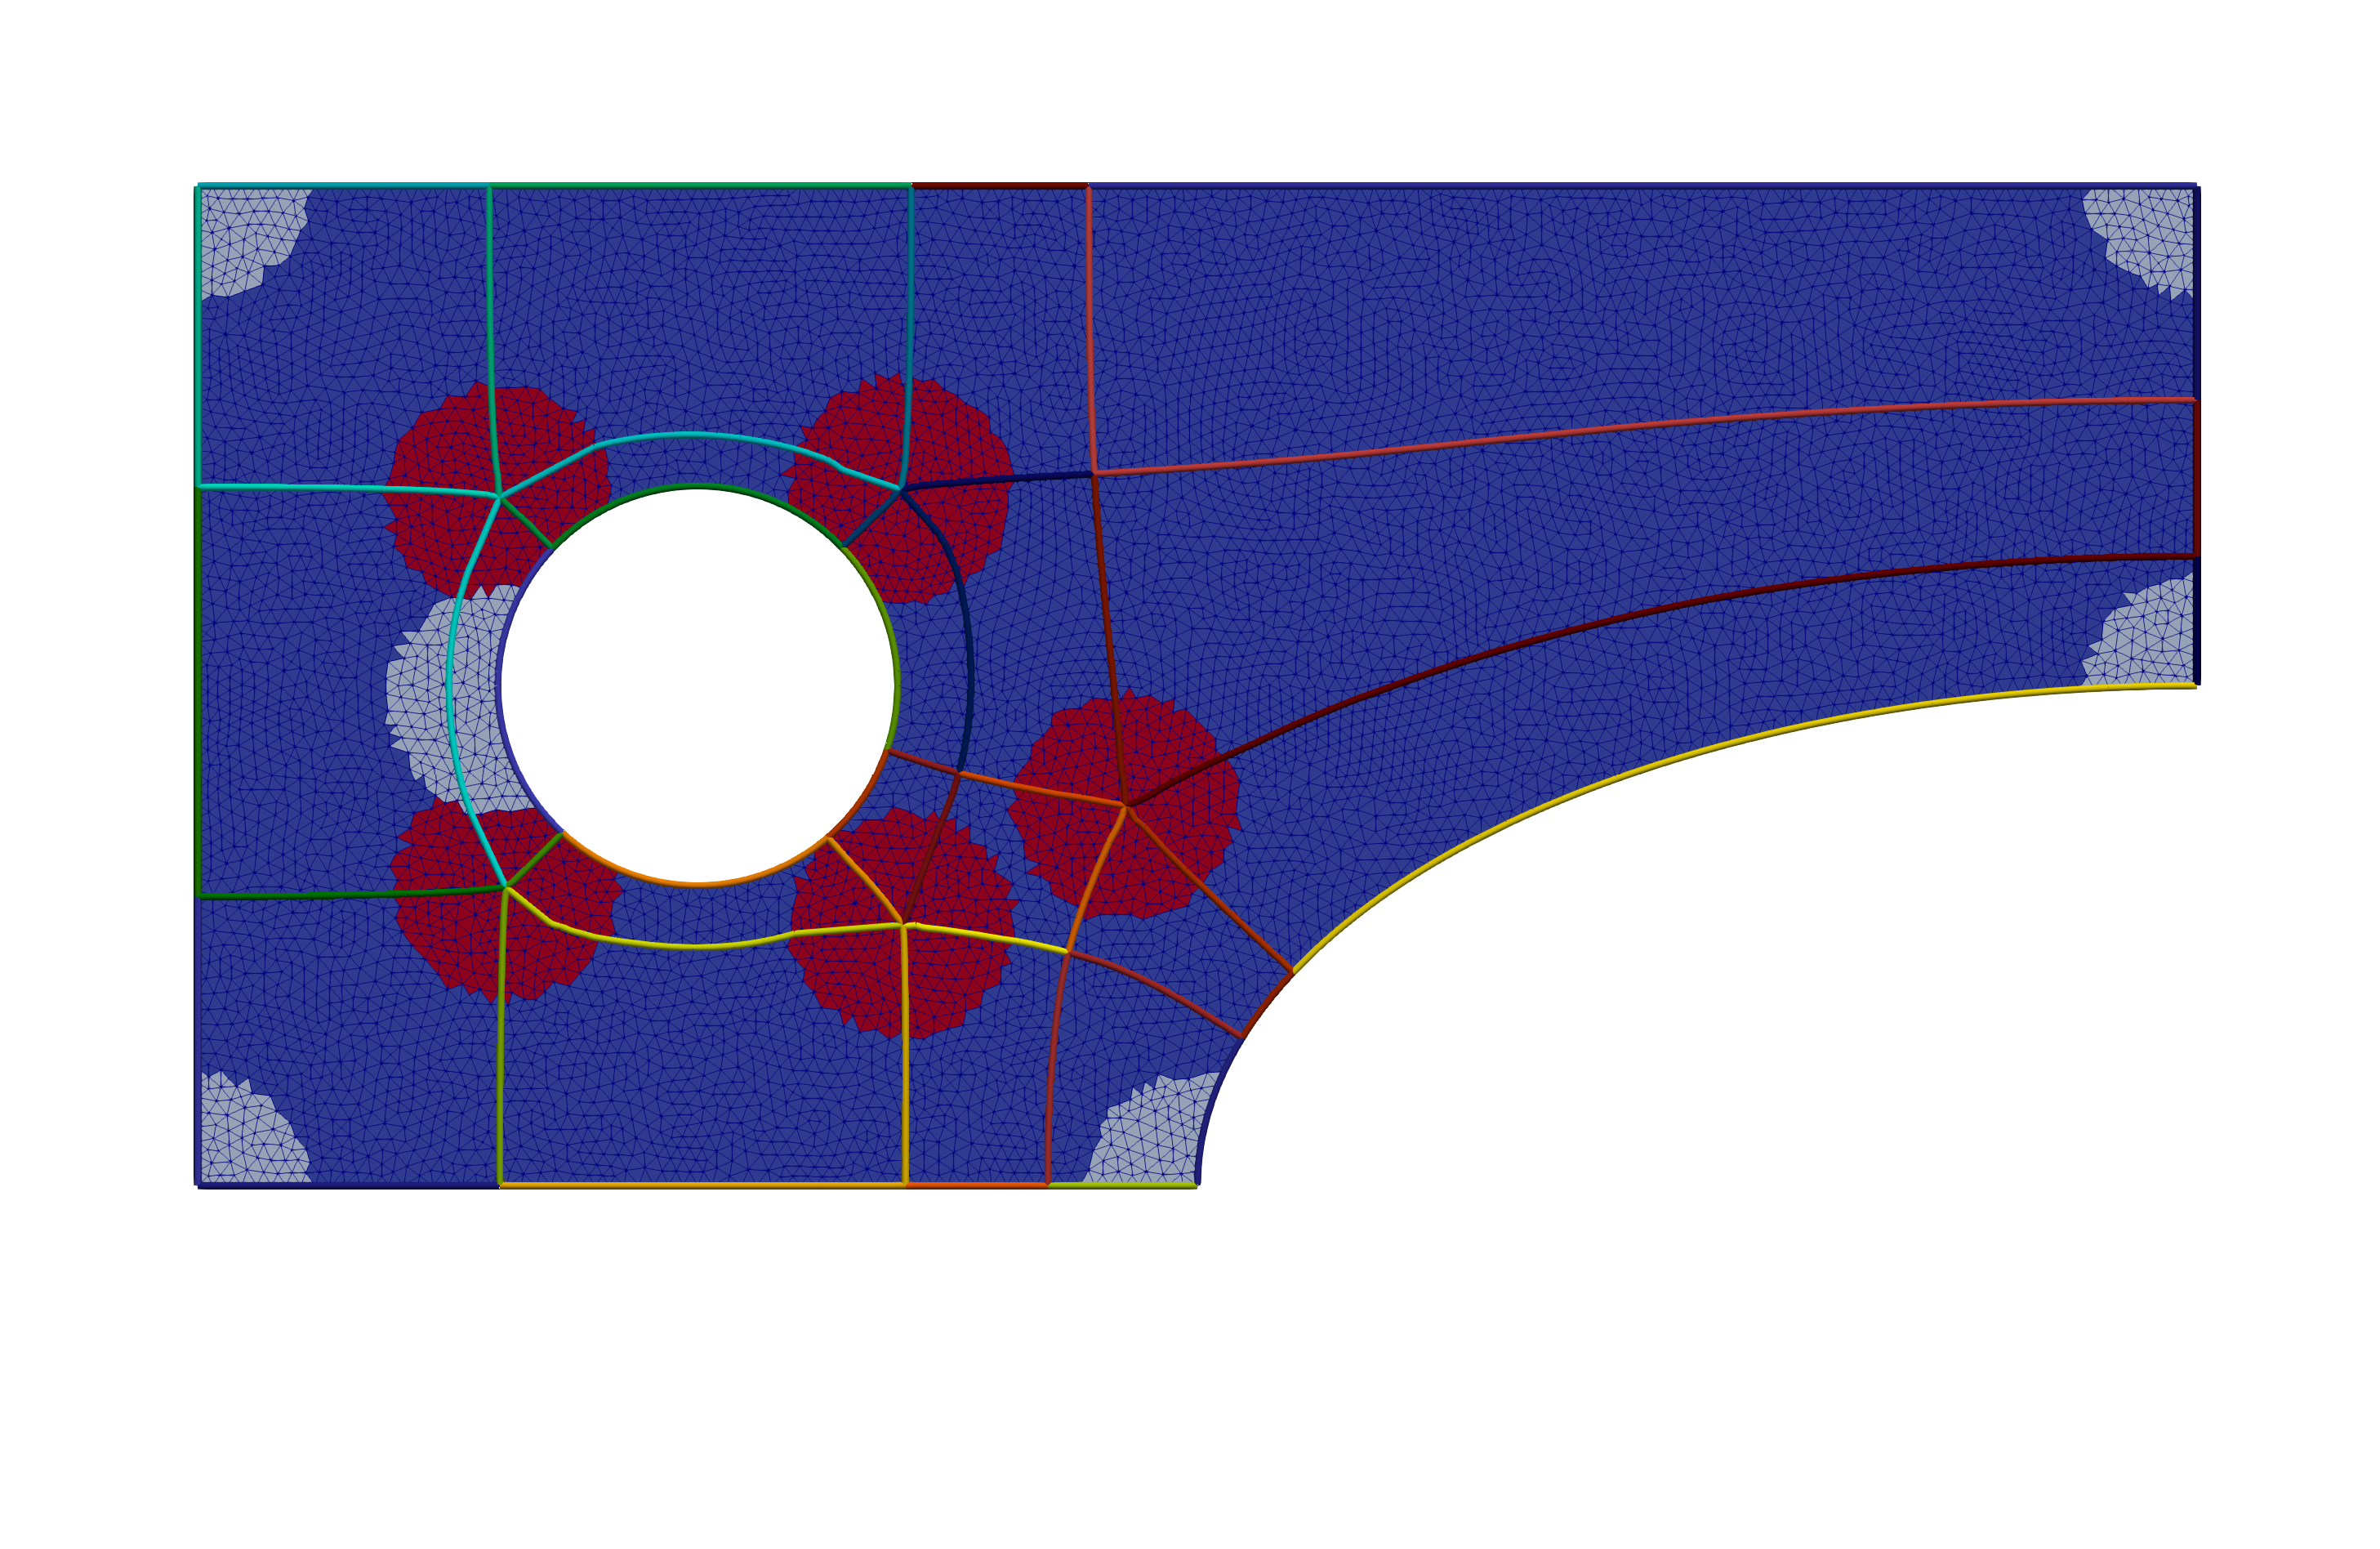
\includegraphics[width=.5\linewidth]
  {img/HIS-SingGraphOriginal-ConfusBallRad005confusBall.png}\hfill 
  \caption{Normal vs very high Radius}
  \end{subfigure}\par\medskip
       % \center{\includegraphics[width=5cm]
        %{img/HIS-SingGraphOriginal-ConfusBallRad001confusBall.png}}
        \caption{ }
      \end{figure}	
     	%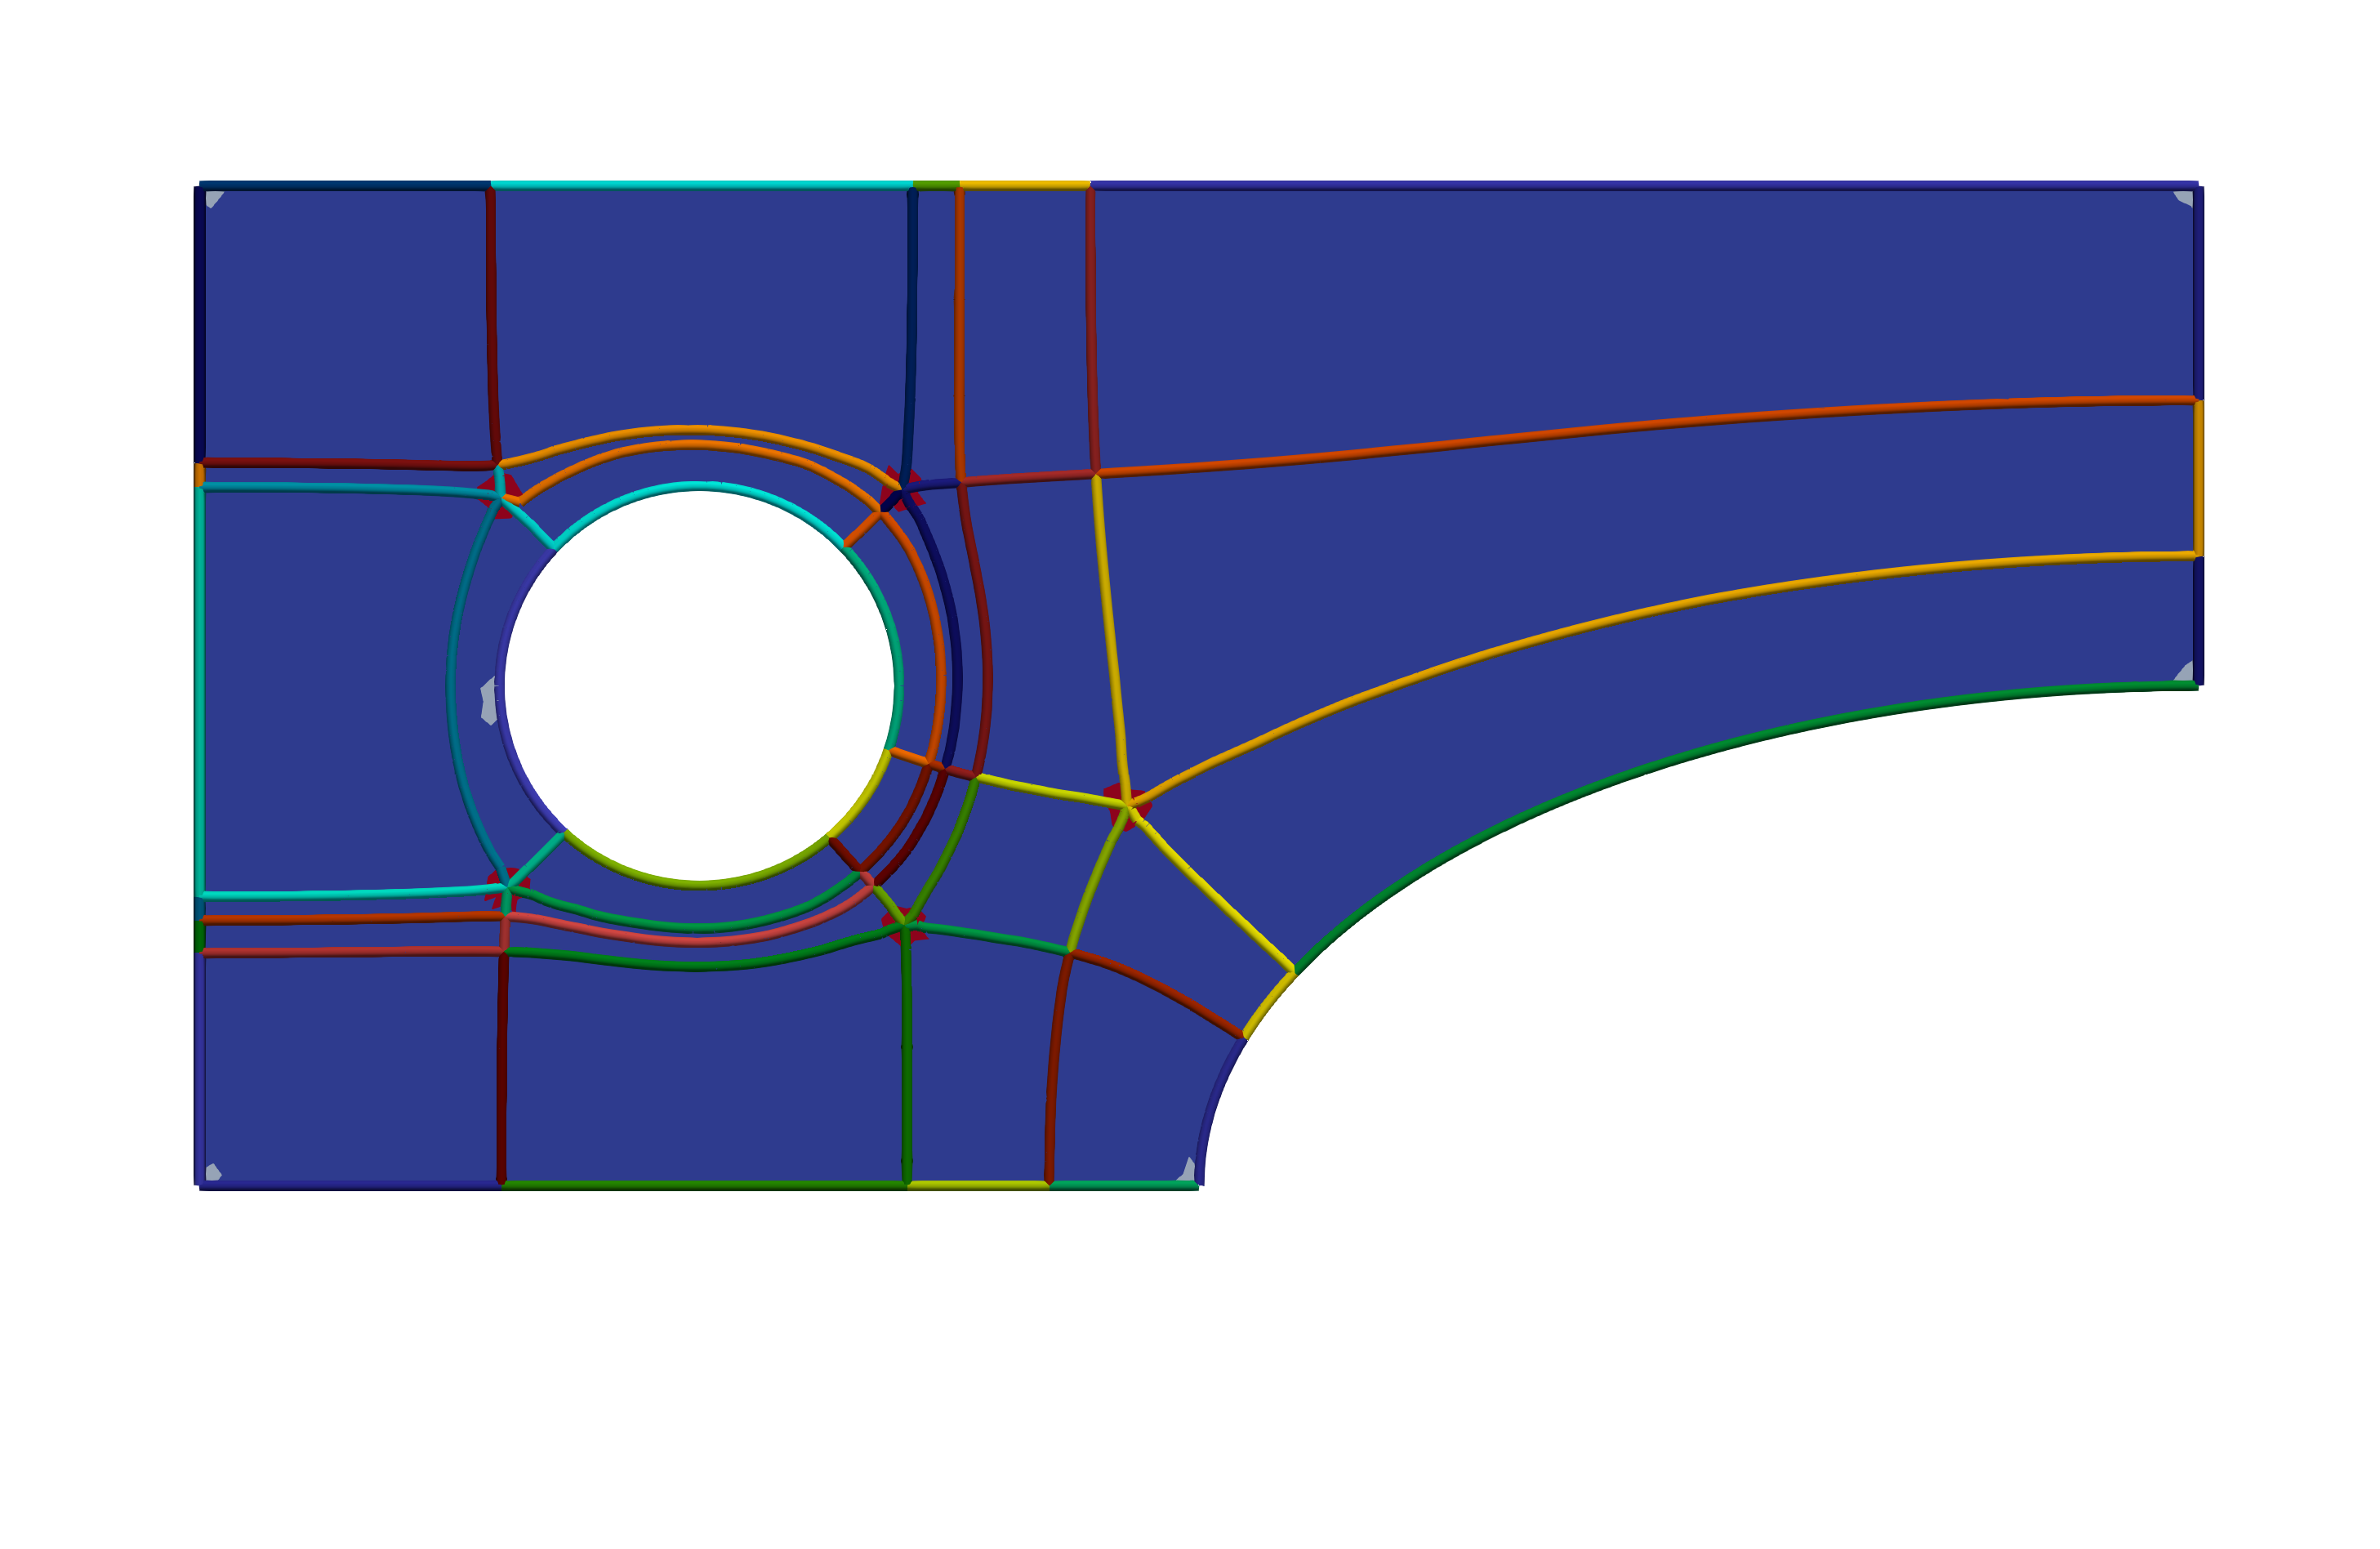
\includegraphics[height=3.7cm]{img/HIS-SingGraphOriginal-ConfusBallRad001confusBall.png}
     	
			
	}
	%%%%%%%%%%%%%%%%%%%%%%%%%%%%%%%%%%%%%%%%%%%%%%%%%%%%%%%%%%%%%%%%%%%%%%%%%%%%%%%%%%%%%%%%
	
	\frame {
		\frametitle{Singularity Graph Building}		
		\framesubtitle{Algorithm Steps}
		%\[\frac{-b \pm \sqrt{b^2 - c}}{2a}\]
		\ \center{B. Simultaneous Strategy}
		\begin{itemize}
			\item 1. Simultaneously depart from each singular point along each slot direction until
			\begin{itemize}
			\item a) reach boundary
			\item b) distance between the current last point added and the last point added for a different line is within a given threshold
			\end{itemize}
			\item 2. If line-line intersection $\Longrightarrow$ treat intersection point as singularity point for the patch layout construction
			
		\end{itemize}
	}
	
%%%%%%%%%%%%%%%%%%%%%%%%%%%%%%%%%%%%%%%%%%%%%%%%%%%%%%%%%%%%%%%%%%%%%%%%%%%%%%%%%%%%%%%%
	\frame {
		\frametitle{Singularity Graph Building}		
		\framesubtitle{Algorithm Steps}
		%\[\frac{-b \pm \sqrt{b^2 - c}}{2a}\]
		\ \center{B. Simultaneous Strategy}
		
		 \begin{figure}[]
        \center{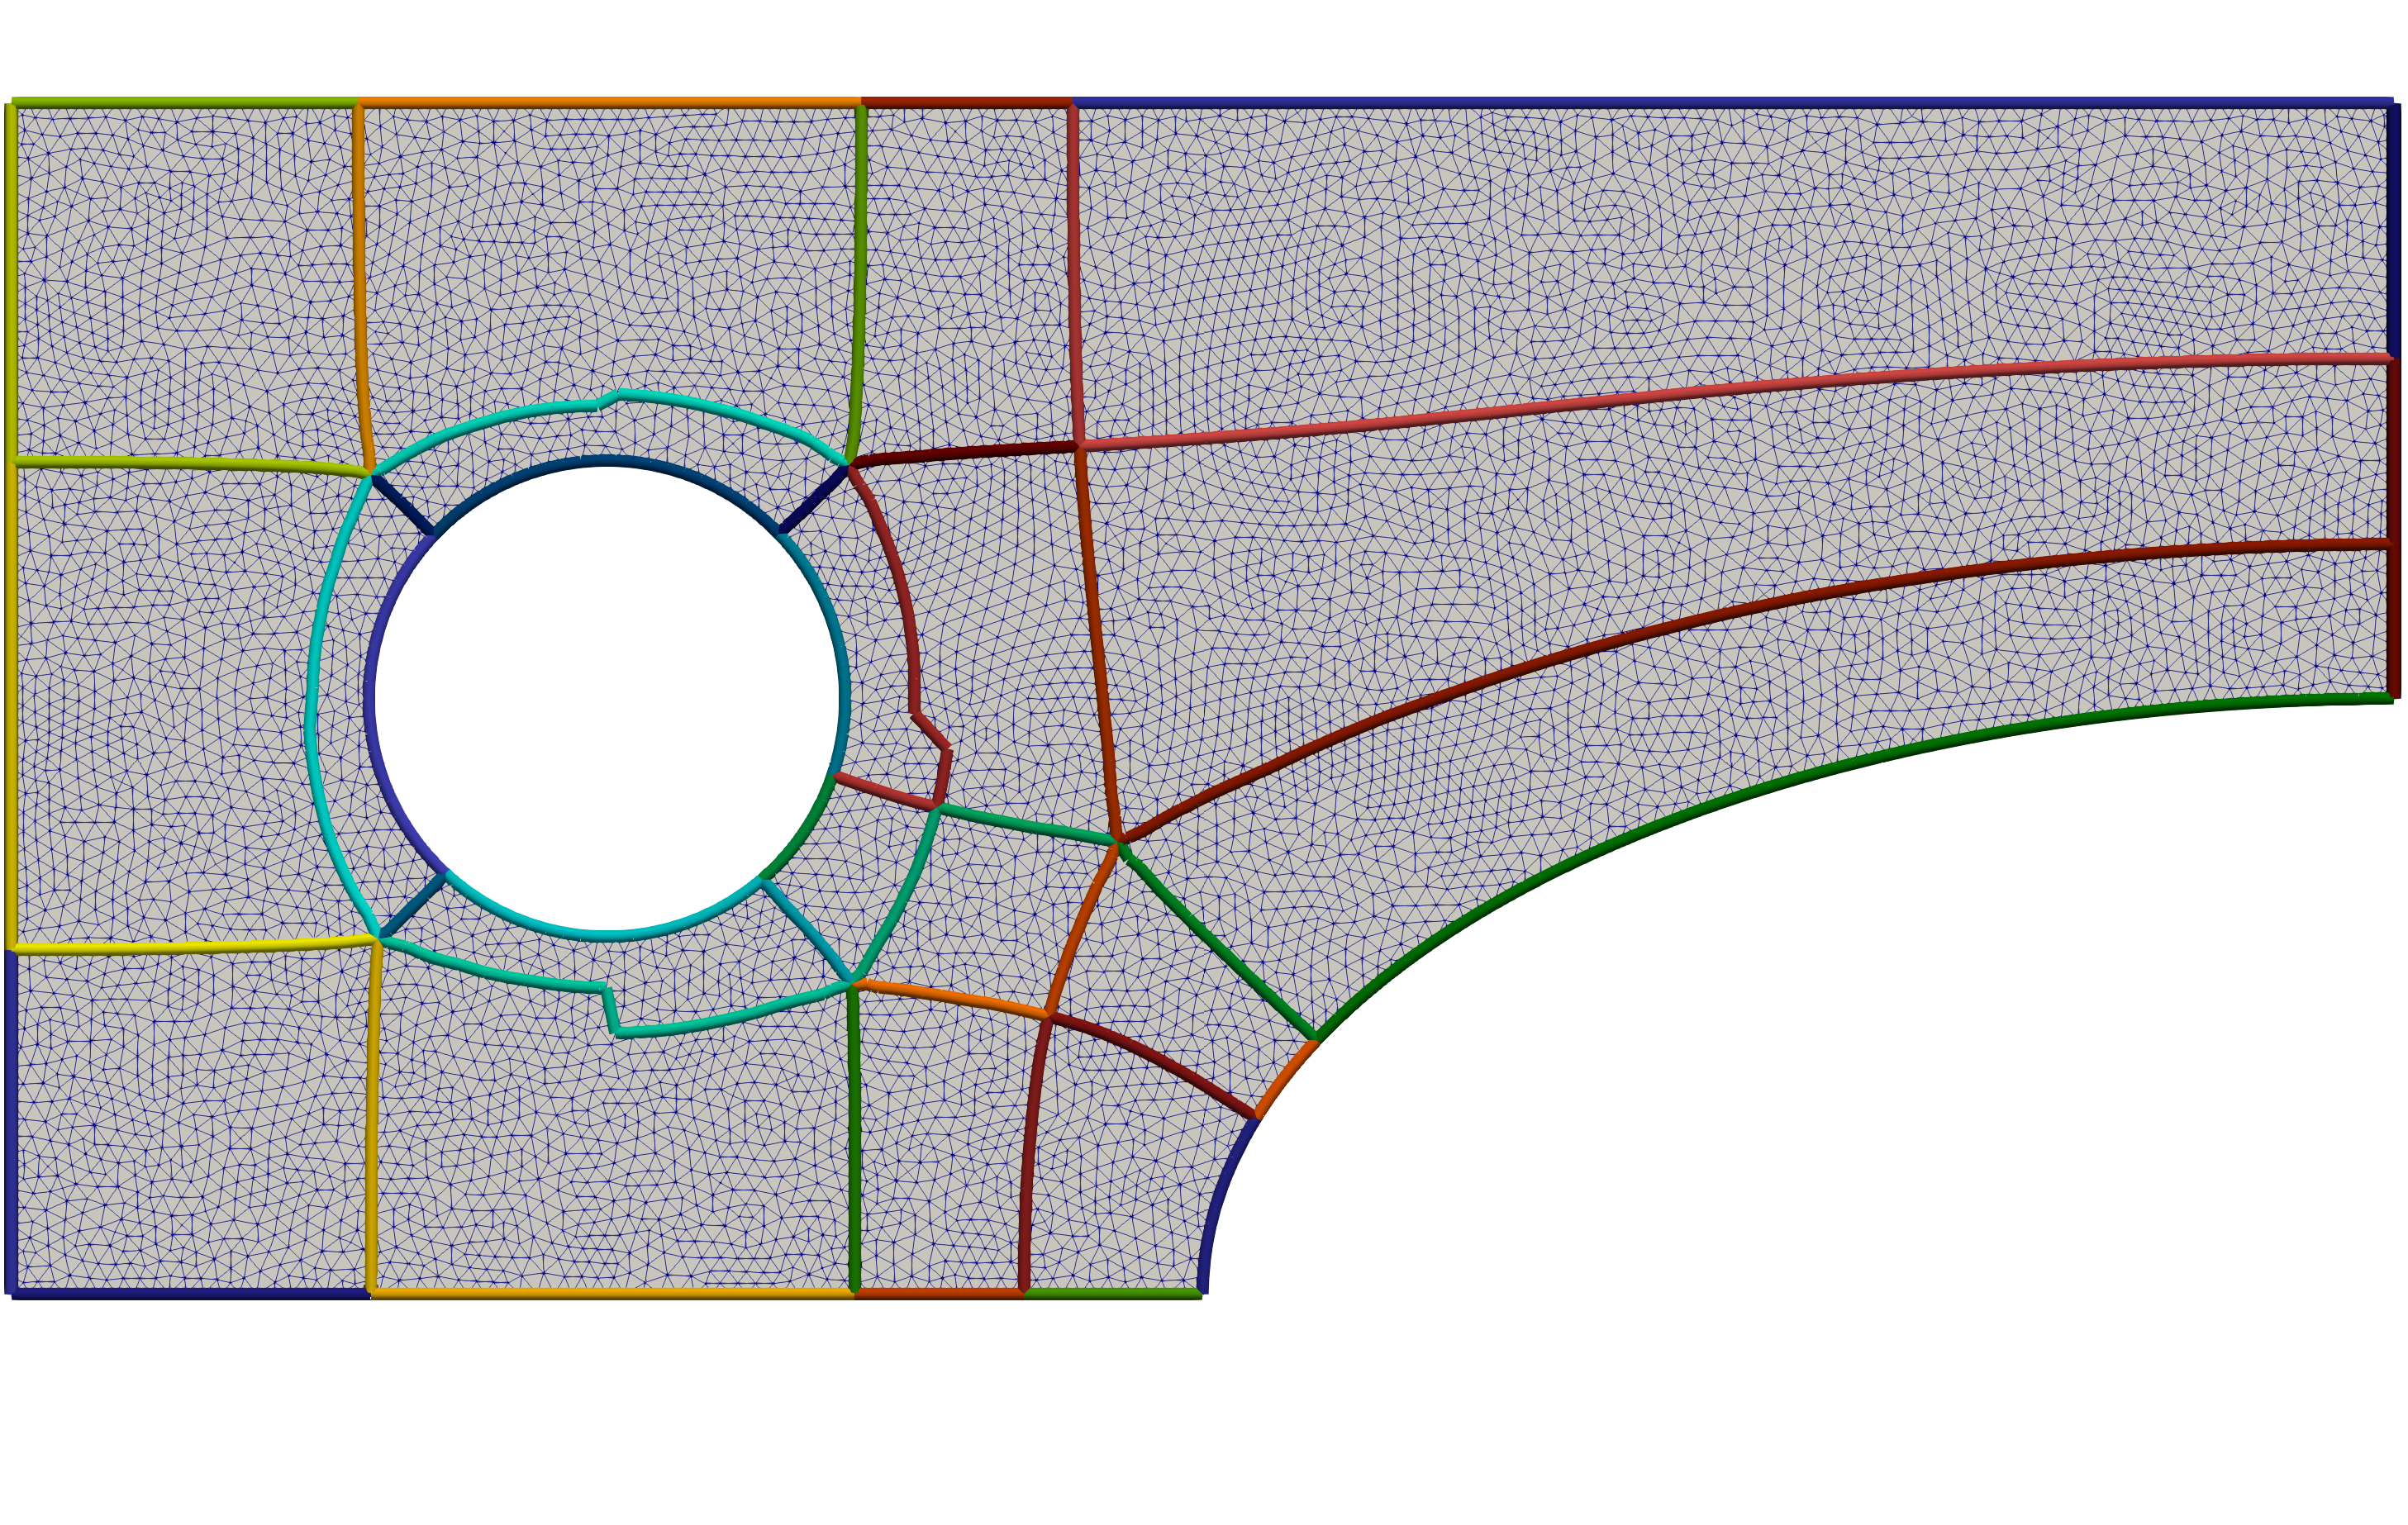
\includegraphics[width=8cm]
        {img/HIS-SingGraphSimultaneous.png}}
        \caption{ Mesh HIS - Singularity Graph}
      \end{figure}	
      %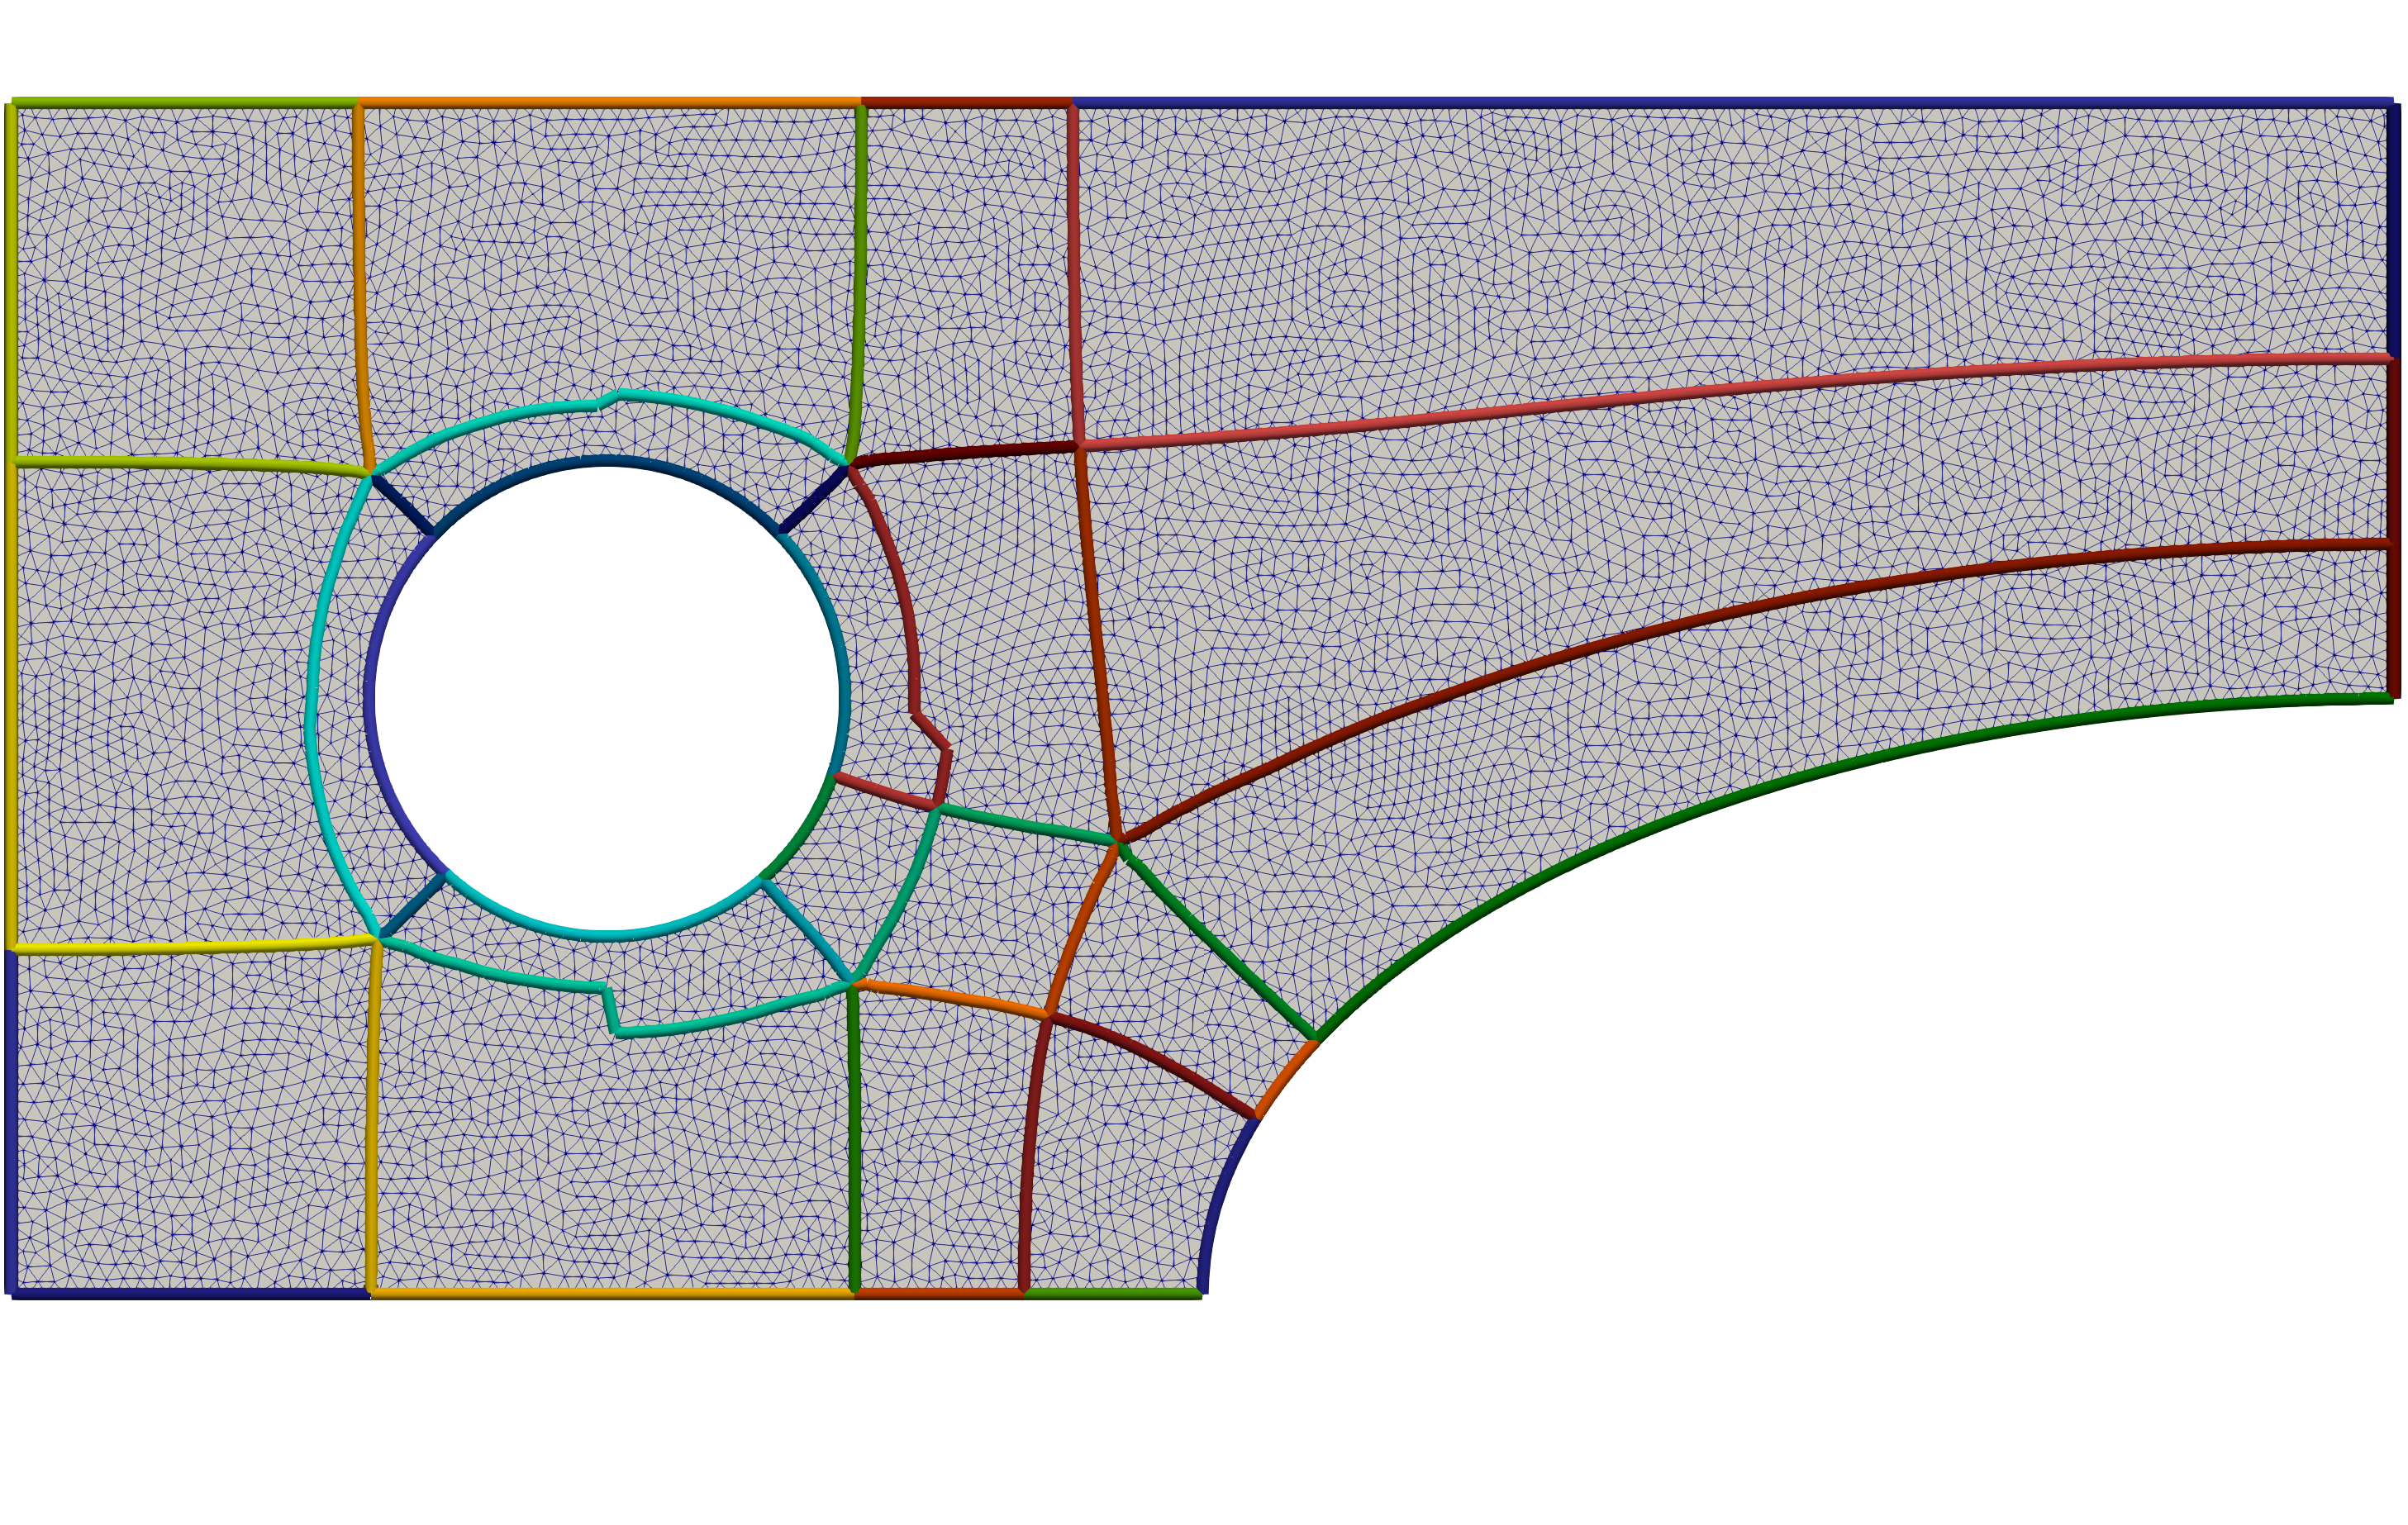
\includegraphics[height=7cm]{img/HIS-SingGraphSimultaneous.png}
     
	}
	
%%%%%%%%%%%%%%%%%%%%%%%%%%%%%%%%%%%%%%%%%%%%%%%%%%%%%%%%%%%%%%%%%%%%%%%%%%%%%%%%%%%%%%%%	
	\frame {
		\frametitle{Singularity Graph Building}		
		\framesubtitle{Algorithm Steps}
		%\[\frac{-b \pm \sqrt{b^2 - c}}{2a}\]
		\ \center{A. Sequential Strategy}
		
		 \begin{table}[]
\begin{tabular}{lllll}
\textbf{Mesh file} & \textbf{|T|}& \textbf{Success/Fail} &  \textbf{Comments} & \textbf{Timing[ms]} \\
  HolesInSquare & 411K & Success  & not as expected  &   76614 \\
   HolesInSquare & 162K & Fail  & not as expected  &   - \\
    HolesInSquare & 100K & Success  & not as expected  &   22291 \\
     HolesInSquare & 41K & Fail  & -  &   - \\
     HolesInSquare & 12K & Success  & not as expected  &   4163 \\
     HolesInSquare & 7K & Success  & not as expected  &   3066 \\     
     HolesInSquare & 2K & Fail  & -  &   - \\     
     HolesInSquare & 770 & Success  & as expected  &   1523 \\     
     HolesInSquare & 416 & Success  & not all singularities  &   1504 
  
\end{tabular}
\end{table}
     
	}
%%%%%%%%%%%%%%%%%%%%%%%%%%%%%%%%%%%%%%%%%%%%%%%%%%%%%%%%%%%%%%%%%%%%%%%%%%%%%%%%%%%%%%%%	
	
	\frame {
		\frametitle{Singularity Graph Building}		
		\framesubtitle{Algorithm Steps}
		%\[\frac{-b \pm \sqrt{b^2 - c}}{2a}\]
		\ \center{A. Simultaneous Strategy}
		
		 \begin{table}[]
\begin{tabular}{lllll}
\textbf{Mesh file} & \textbf{|T|}& \textbf{Success/Fail} &  \textbf{Comments} & \textbf{Timing[ms]} \\
  HolesInSquare & 411K & Fail  & -  &   - \\
   HolesInSquare & 162K & Success  & 60\% of cases  &   - \\
    HolesInSquare & 100K & Success  & 20\% of cases &   - \\
     HolesInSquare & 41K & Success  & 60\% of cases  &   - \\
     HolesInSquare & 12K & Success  & 100\% of cases  &   3368 \\
     
     HolesInSquare & 7K & Success  & 100\% of cases  &   1957 \\
         
     HolesInSquare & 2K & Success  & 20\% of cases  &   - \\  
        
     HolesInSquare & 770 & Success  & 20\% of cases  &   - \\     
     HolesInSquare & 416 & Success  & 40\% of cases  &   - 
  
\end{tabular}
\end{table}
     
	}
	
%%%%%%%%%%%%%%%%%%%%%%%%%%%%%%%%%%%%%%%%%%%%%%%%%%%%%%%%%%%%%%%%%%%%%%%%%%%%%%%%%%%%%%%%
	
	\frame{

\begin{tabular}{ |l|l|l|l| }
\hline
\multirow{3}{*}{Mesh} & Connecting  & \multirow{3}{*}{Output}  & \multirow{3}{*}{Comments} \\
 & Threshold & & \\
 & Distance & & \\ \hline
\multirow{5}{*}{HIS0} & 1*SS & \textcolor{green}{OK(19F)}& \\
& 2*SS & \textcolor{green}{OK(19F)} & \\
 & 3*SS &  \textcolor{red}{FAIL} & \\
 & 4*SS &  \textcolor{red}{FAIL} & \\
 & 5*SS &    \textcolor{red}{FAIL} & \\ \hline
 
\multirow{5}{*}{HIS1} & 1*SS & \textcolor{red}{FAIL } & \\ %- segmentation error
& 2*SS &  \textcolor{green}{OK(16F)} & \\
 & 3*SS &  \textcolor{red}{FAIL}  & \\
 & 4*SS & \textcolor{red}{FAIL} & \\
 & 5*SS &   \textcolor{red}{FAIL}& \\ \hline
 
  \multirow{5}{*}{HIS2} & 1*SS & \textcolor{red}{FAIL} & \\ %- segmentation error
& 2*SS &  \textcolor{green}{OK(19F)}& \\
 & 3*SS &   \textcolor{red}{BAD(16F)}& not as expected \\
 & 4*SS &  \textcolor{red}{BAD(16F)}& not as expected\\
 & 5*SS &   \textcolor{red}{BAD(13F)}& not as expected\\ \hline
\end{tabular}	
	}
	
	%%%%%%%%%%%%%%%%%%%%%%%%%%%%%%%%%%%%%%%%%%%%%%%%%%%%%%%%%%%%%%%%%%%%%%%%%%%%%%%%%%%%%%%%
		\frame{
\begin{tabular}{ |l|l|l|l| }
\hline
\multirow{3}{*}{Mesh} & Connecting  & \multirow{3}{*}{Output}  & \multirow{3}{*}{Comments} \\
 & Threshold & & \\
 & Distance & & \\ \hline

 
 \multirow{5}{*}{HIS3} & 1*SS &  \textcolor{green}{OK(19F)} &\\
& 2*SS &   \textcolor{green}{OK(19F)}&\\
 & 3*SS &  \textcolor{green}{OK(19F)}& \\
 & 4*SS &  \textcolor{green}{OK(19F)}&\\
 & 5*SS &  \textcolor{green}{OK(19F)} &\\ \hline
 
 \multirow{5}{*}{HIS4} & 1*SS &  \textcolor{green}{OK(24F)}& \\
& 2*SS &  \textcolor{green}{OK(19F)}&\\
 & 3*SS &   \textcolor{green}{OK(19F)}&\\
 & 4*SS & \textcolor{green}{OK(19F)} &\\
 & 5*SS &  \textcolor{green}{OK(19F)}  &\\ \hline
  \multirow{5}{*}{HIS5} & 1*SS &  \textcolor{red}{FAIL} & \\
& 2*SS &  \textcolor{red}{FAIL} & cycle + streamlineCrossing\\
 & 3*SS &  \textcolor{green}{OK(19F)} &\\
 & 4*SS &  \textcolor{green}{OK(19F)} -//-&\\
 & 5*SS &   \textcolor{green}{OK(19F)}&\\ \hline

\end{tabular}	
}


%%%%%%%%%%%%%%%%%%%%%%%%%%%%%%%%%%%%%%%%%%%%%%%%%%%%%%%%%%%%%%%%%%%%%%%%%%%%%%%%%%%%%%%%
	\frame{
\begin{tabular}{ |l|l|l|l|}
\hline
\multirow{3}{*}{Mesh} & Connecting  & \multirow{3}{*}{Output}  & \multirow{3}{*}{Comments} \\
 & Threshold & & \\
 & Distance & & \\ \hline
 

 
   \multirow{5}{*}{HIS6} & 1*SS & \textcolor{red}{BAD(29F)} & streamlineCrossing\\
& 2*SS &  \textcolor{red}{BAD(29F)}&streamlineCrossing \\
 & 3*SS &   \textcolor{red}{BAD(22F)} &streamlineCrossing\\
 & 4*SS &   \textcolor{red}{BAD(22F)}&streamlineCrossing\\
 & 5*SS &  \textcolor{green}{OK(19F)} &\\ \hline
 
  \multirow{5}{*}{HIS7} & 1*SS & \textcolor{red}{BAD(21F)} & streamlineCrossing\\
& 2*SS &  \textcolor{red}{BAD(21F)}& streamlineCrossing\\
 & 3*SS & \textcolor{green}{OK(21F)} - -//- &\\
 & 4*SS & \textcolor{green}{OK(19F)}) &\\
 & 5*SS & \textcolor{green}{OK(19F)} -//- &\\ \hline
 
  \multirow{5}{*}{HIS8} & 1*SS & \textcolor{red}{BAD(17F)} &  connectingThreshDist - too small\\ %intersection
& 2*SS &   \textcolor{red}{BAD(22F)} & connectingThreshDist - too small\\%intersection
 & 3*SS &  \textcolor{red}{BAD(22F)} & connectingThreshDist - too small \\%intersection
 & 4*SS &  \textcolor{red}{FAIL}& connectingThreshDist - too small\\
 & 5*SS &  \textcolor{red}{FAIL} & connectingThreshDist - too small\\ \hline
\end{tabular}
}



%%%%%%%%%%%%%%%%%%%%%%%%%%%%%%%%%%%%%%%%%%%%%%%%%%%%%%%%%%%%%%%%%%%%%%%%%%%%%%%%%%%%%%%%%%%
	

\frame{

\begin{tabular}{ |l|l|l|l|}
\hline
\multirow{3}{*}{Mesh} & Connecting  & \multirow{3}{*}{Output}  & \multirow{3}{*}{Comments} \\
 & Threshold & & \\
 & Distance & & \\ \hline
 
 \multirow{5}{*}{Circle\_ref} & 1*SS &  \textcolor{red}{BAD} & \\
& 2*SS &  \textcolor{green}{OK(5F)} &\\
 & 3*SS &  \textcolor{green}{OK(5F)} &\\
 & 4*SS &  \textcolor{green}{OK(5F)} &\\
 & 5*SS &   \textcolor{green}{OK(5F)} & -//-\\ \hline
 
   \multirow{5}{*}{Circle\_coarse} & 1*SS &  \textcolor{green}{OK(5F)} & \\
& 2*SS &   \textcolor{green}{OK(5F)}& \\
 & 3*SS &   \textcolor{green}{OK(5F)} & \\
 & 4*SS &  \textcolor{red}{FAIL} & seg error\\
 & 5*SS &  \textcolor{red}{FAIL} & seg error\\ \hline


   \multirow{5}{*}{Circle\_with\_circle\_holes\_coarse} & 1*SS &  \textcolor{red}{BAD} & cycle \\
& 2*SS &   \textcolor{red}{BAD} & cycle\\
 & 3*SS &   \textcolor{red}{BAD} & cycle\\
 & 4*SS &  \textcolor{red}{FAIL} & seg error in patch constr, but no cycle\\
 & 5*SS &  \textcolor{red}{FAIL} & seg error in patch constr, but no cycle\\ \hline
 
 
 
\end{tabular}

}


%%%%%%%%%%%%%%%%%%%%%%%%%%%%%%%%%%%%%%%%%%%%%%%%%%%%%%%%%%%%%%%%%%%%%%%%%%%%%%%%%%%%%%%%
\frame{
\begin{tabular}{ |l|l|l|l|}
\hline
\multirow{3}{*}{Mesh} & Connecting  & \multirow{3}{*}{Output}  & \multirow{3}{*}{Comments} \\
 & Threshold & & \\
 & Distance & & \\ \hline
 
 \multirow{5}{*}{Circle\_with\_circle\_holes\_ref} & 1*SS &  \textcolor{red}{BAD} & cycle \\
& 2*SS &   \textcolor{red}{BAD} &  cycle \\
 & 3*SS &   \textcolor{red}{BAD} & seg error in patch constr and streamlineCrossing \\
 & 4*SS &  \textcolor{red}{BAD} & seg error in patch constr and streamlineCrossing \\
 & 5*SS &  \textcolor{red}{BAD} & seg error in patch constr and streamlineCrossing \\ \hline
 
   \multirow{5}{*}{Circle\_with\_concavities\_coarse} & 1*SS &  \textcolor{green}{OK} & problem in patch constr \\
& 2*SS &    \textcolor{green}{OK} & -//- \\
 & 3*SS &   \textcolor{green}{OK} & problem in patch constr \\
 & 4*SS &  \textcolor{green}{OK} & problem in patch constr\\
 & 5*SS &  \textcolor{green}{OK} & problem in patch constr \\ \hline
 
  \multirow{5}{*}{Circle\_with\_concavities} & 1*SS &  \textcolor{red}{BAD} & problem in patch constr \\
& 2*SS &   \textcolor{red}{BAD} &  -//- (problem is field) \\
 & 3*SS &   \textcolor{red}{BAD} & streamlines outside of mesh \\
 & 4*SS &  \textcolor{red}{BAD} &  streamlines outside of mesh \\
 & 5*SS &  \textcolor{red}{BAD} &  streamlines outside of mesh \\ \hline
 
\end{tabular}
}

%%%%%%%%%%%%%%%%%%%%%%%%%%%%%%%%%%%%%%%%%%%%%%%%%%%%%%%%%%%%%%%%%%%%%%%%%%%%%%%%%%%%%%%%
\frame{
\begin{tabular}{ |l|l|l|l|}
\hline
\multirow{3}{*}{Mesh} & Connecting  & \multirow{3}{*}{Output}  & \multirow{3}{*}{Comments} \\
 & Threshold & & \\
 & Distance & & \\ \hline

 \multirow{5}{*}{Circle\_with\_concavities\_ref} & 1*SS &  \textcolor{green}{OK} & problem in patch constr \\
& 2*SS &    \textcolor{green}{OK} &  -//- (problem is field) \\
 & 3*SS &    \textcolor{green}{OK} & streamlines outside of mesh \\
 & 4*SS &  \textcolor{green}{OK} &  streamlines outside of mesh \\
 & 5*SS &  \textcolor{green}{OK} &  streamlines outside of mesh \\ \hline
 
 \multirow{5}{*}{Curved\_Shape1} & 1*SS &  \textcolor{red}{FAIL} & problem in line inters \\
& 2*SS &    \textcolor{green}{OK} &  problem in patch constr \\
 & 3*SS &    \textcolor{green}{OK} & problem in patch constr \\
 & 4*SS &  \textcolor{green}{OK} &  problem in patch constr \\
 & 5*SS &  \textcolor{green}{OK} &  problem in patch constr \\ \hline

 \multirow{5}{*}{Curved\_Shape1\_ref} & 1*SS &  \textcolor{red}{FAIL} & bug - to check \\
& 2*SS &    \textcolor{green}{OK} &  problem in line inters \\
 & 3*SS &    \textcolor{green}{OK} & problem in line inters \\
 & 4*SS &  \textcolor{green}{OK} &  problem in line inters \\
 & 5*SS &  \textcolor{green}{OK} &  problem in patch constr \\ \hline

\end{tabular}

}

%%%%%%%%%%%%%%%%%%%%%%%%%%%%%%%%%%%%%%%%%%%%%%%%%%%%%%%%%%%%%%%%%%%%%%%%%%%%%%%%%%%%%%%%

\frame{
\begin{tabular}{ |l|l|l|l|}
\hline
\multirow{3}{*}{Mesh} & Connecting  & \multirow{3}{*}{Output}  & \multirow{3}{*}{Comments} \\
 & Threshold & & \\
 & Distance & & \\ \hline
 
  \multirow{5}{*}{shape1} & 1*SS &  \textcolor{green}{OK} & problem in patch constr \\
& 2*SS &    \textcolor{red}{FAIL} &  cycle \\
 & 3*SS &    \textcolor{green}{OK} & problem in patch constr \\
 & 4*SS &  \textcolor{red}{FAIL} &  cycle \\
 & 5*SS &  \textcolor{green}{OK} &  problem in patch constr \\ \hline
 
 \end{tabular}
 }



	\frame{
	\begin{figure}[]
        \center{\includegraphics[width=10cm]
        {img/HIS8-SS1.png}}
        \caption{ Mesh HIS8 - SS1} %\caption{\label{fig:HIS8 - SS1} Mesh HIS8 - SS1}
      \end{figure}
      }
      
      \frame{
	 \begin{figure}[]
        \center{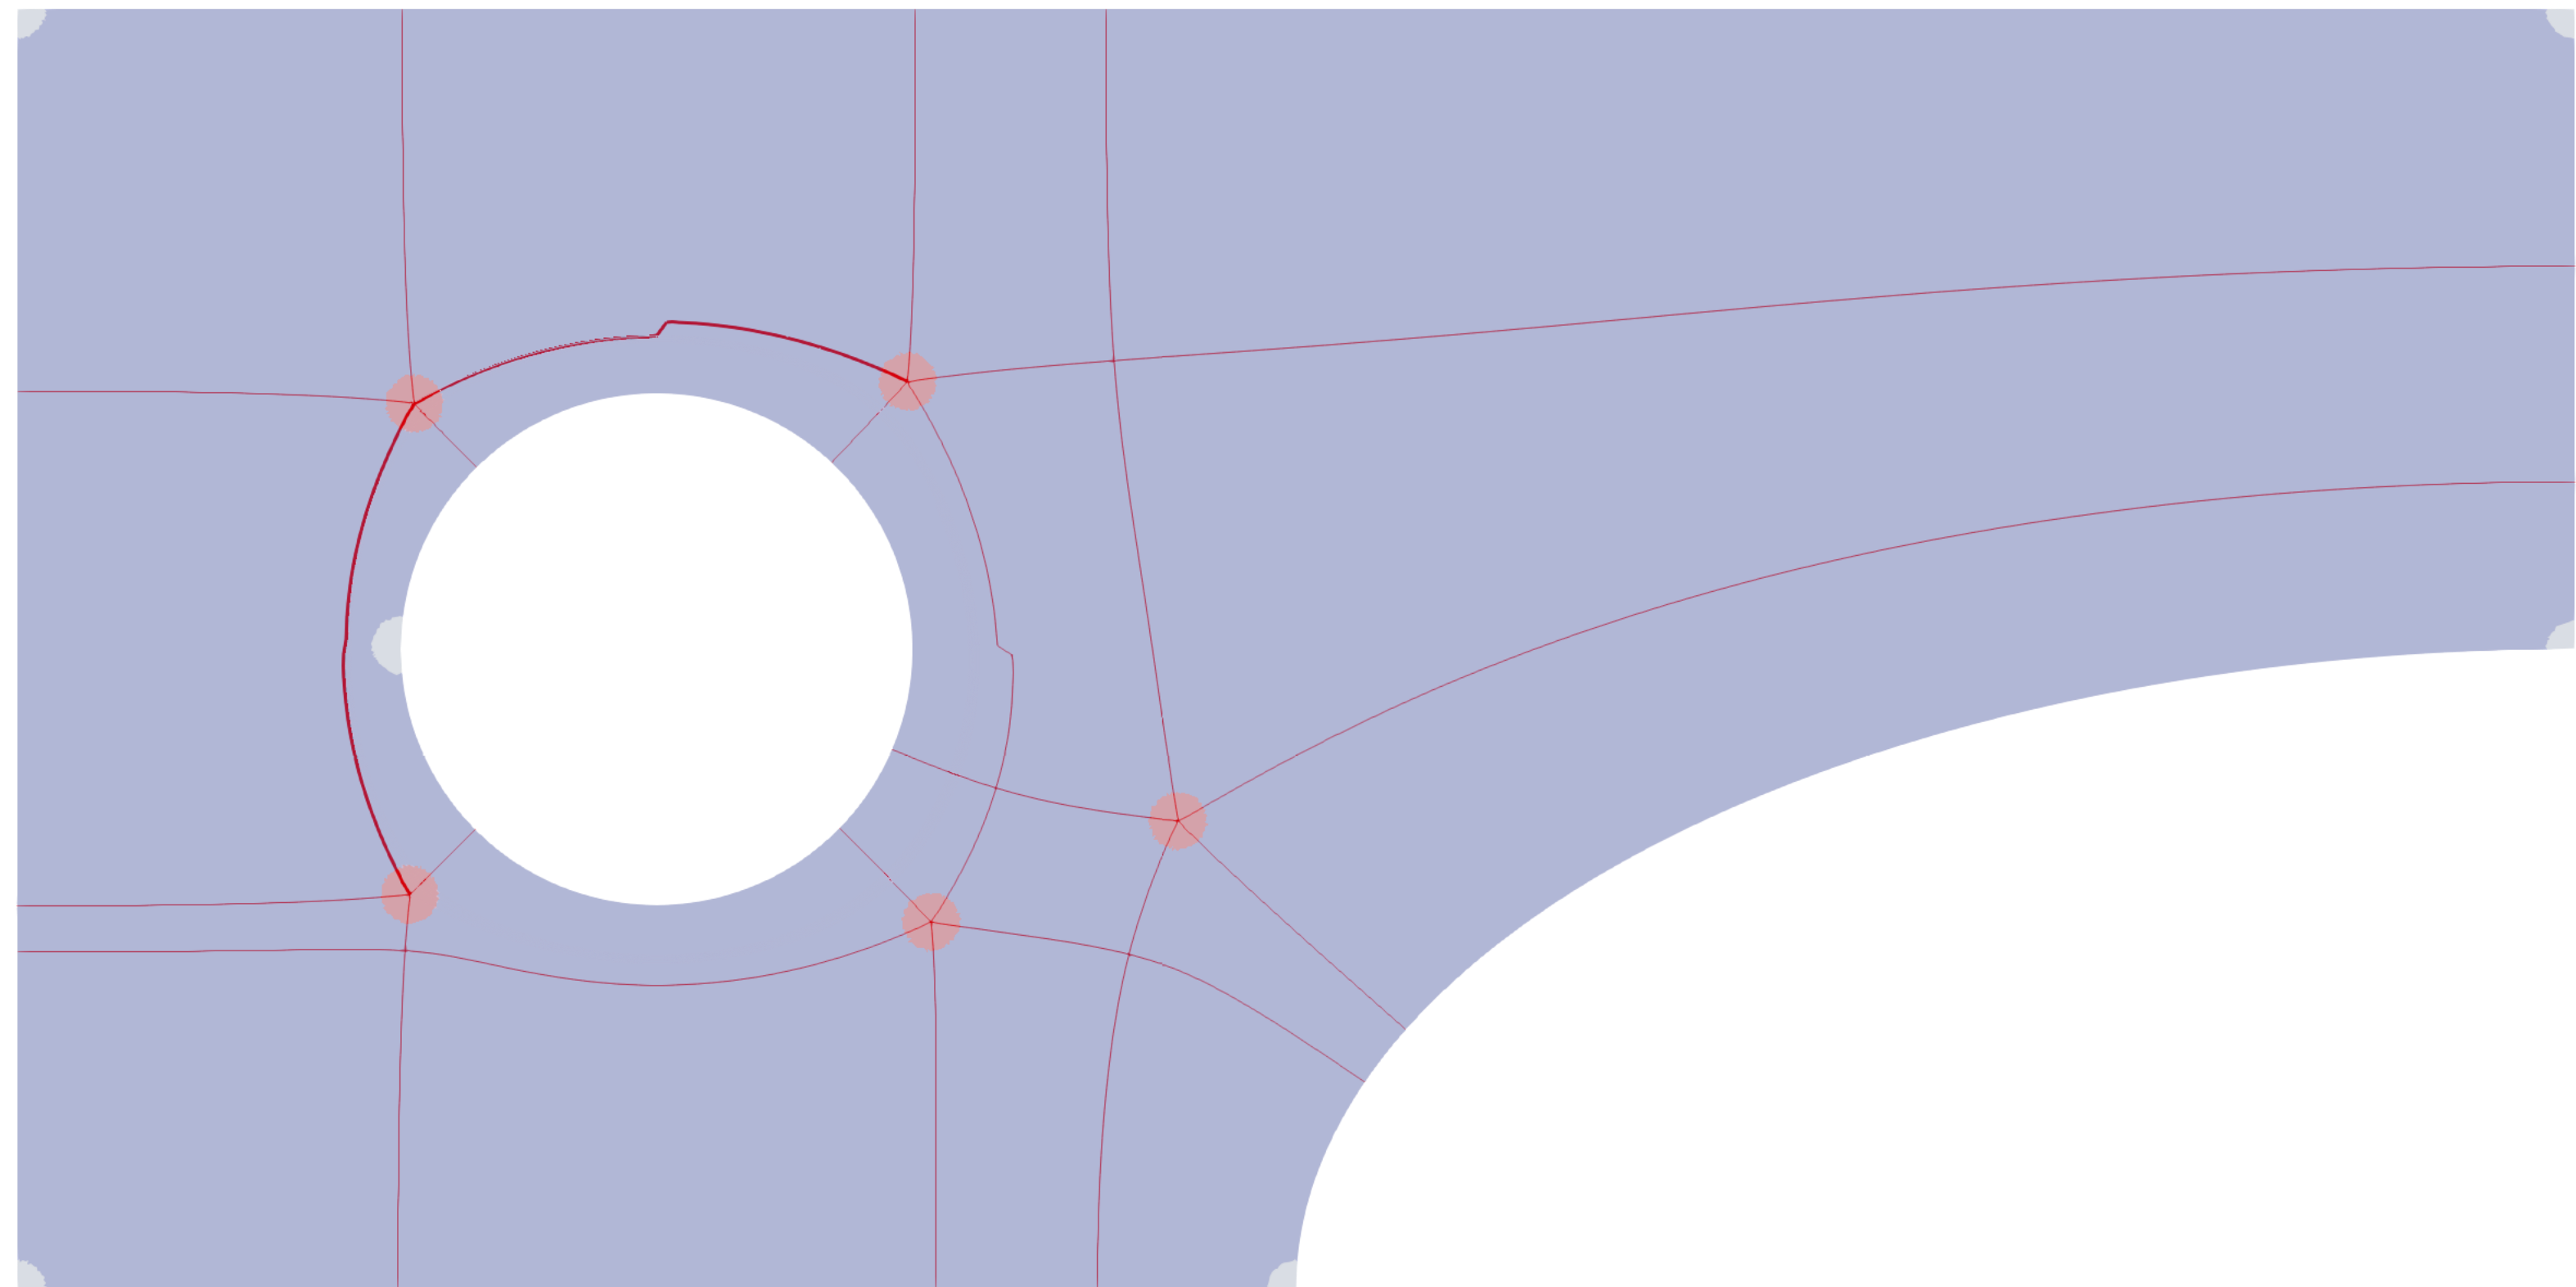
\includegraphics[width=10cm]
        {img/HIS8-SS5.png}}
        \caption{ Mesh HIS8 - SS5}
      \end{figure}
	}
	
	\frame{
	\begin{figure}[]
        \center{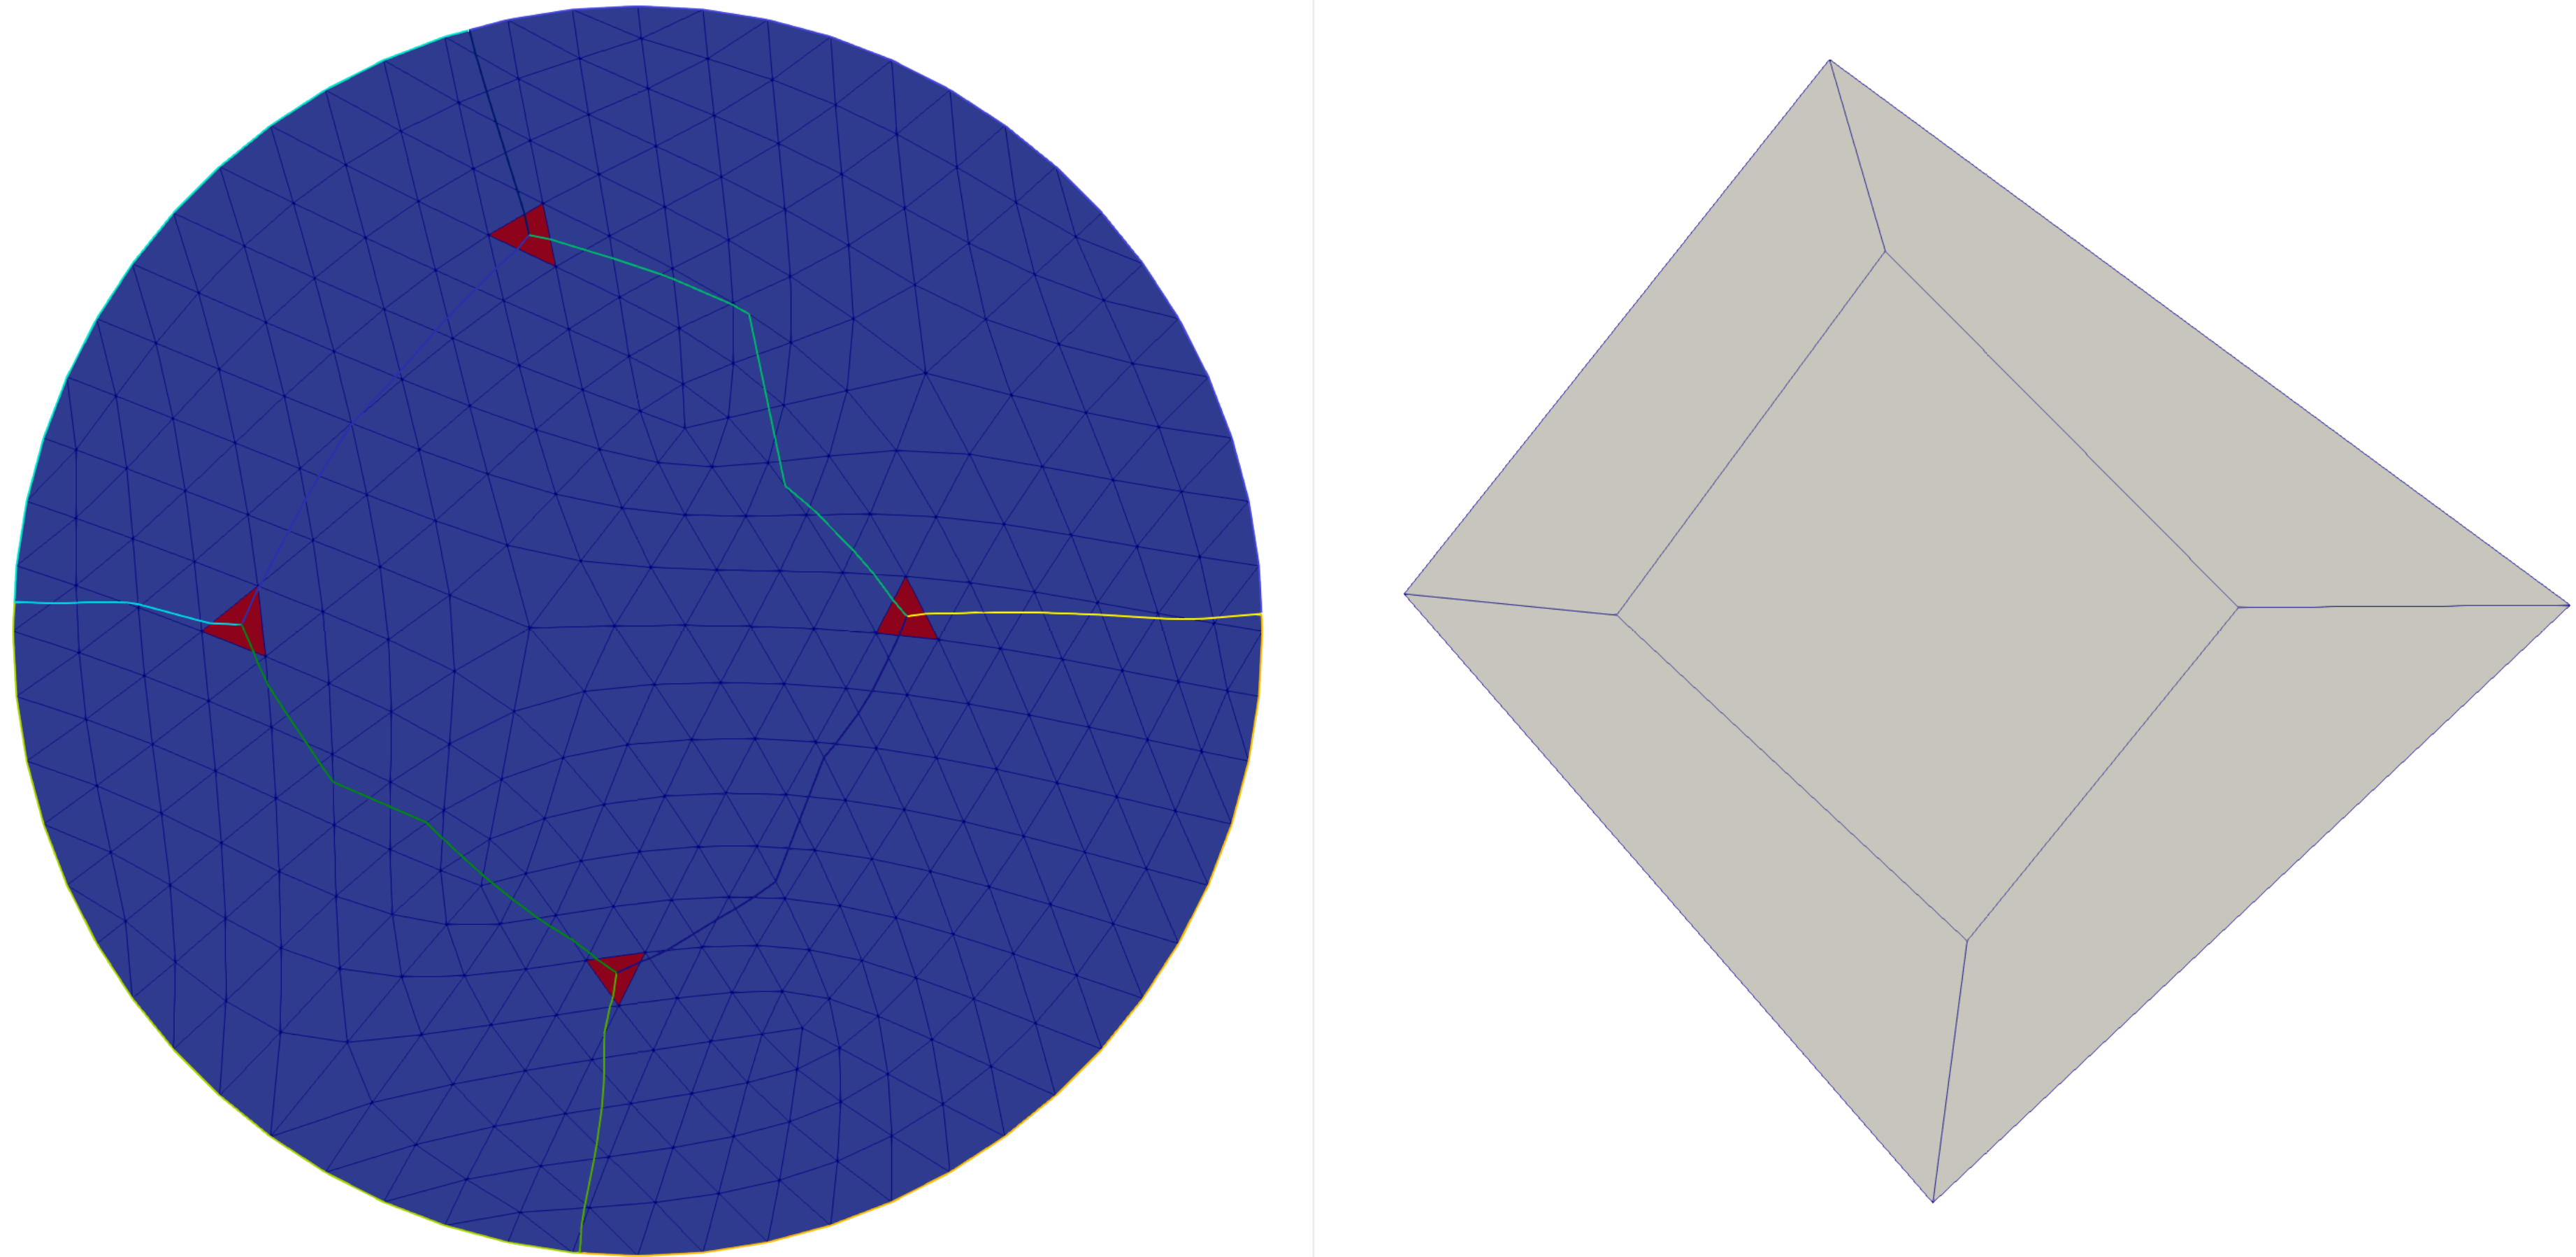
\includegraphics[width=10cm]
        {img/Circle_refSS3.png}}
        \caption{ Mesh Circle\_ref - SS3}
      \end{figure}
	}
	
	\frame{
	\begin{figure}[]
        \center{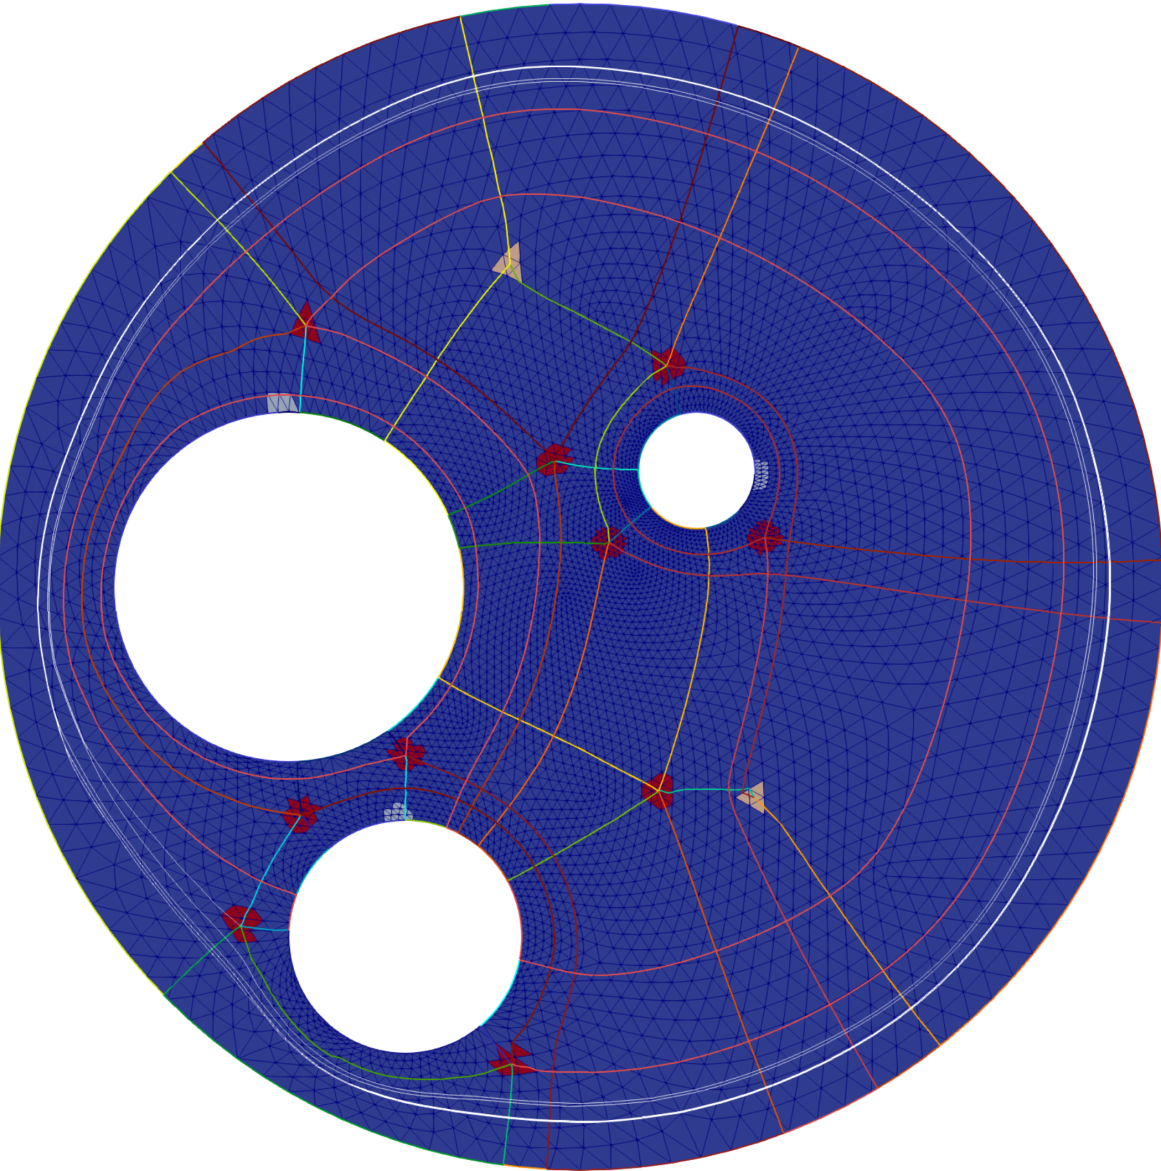
\includegraphics[width=8cm]
        {img/Circle_with_circle_holes_refSS1-cycle.png}}
        \caption{ Mesh Circle\_with\_circle\_holes\_ref - SS1}
      \end{figure}
      }
      
      \frame{
      \begin{figure}[]
        \center{\includegraphics[width=8cm]
        {img/Circle_with_circle_holes_coarseSS4-nocycle.png}}
        \caption{ Mesh Circle\_with\_circle\_holes\_coarse - SS4}
      \end{figure}
      }
      
      \frame{
      \begin{figure}[]
        \center{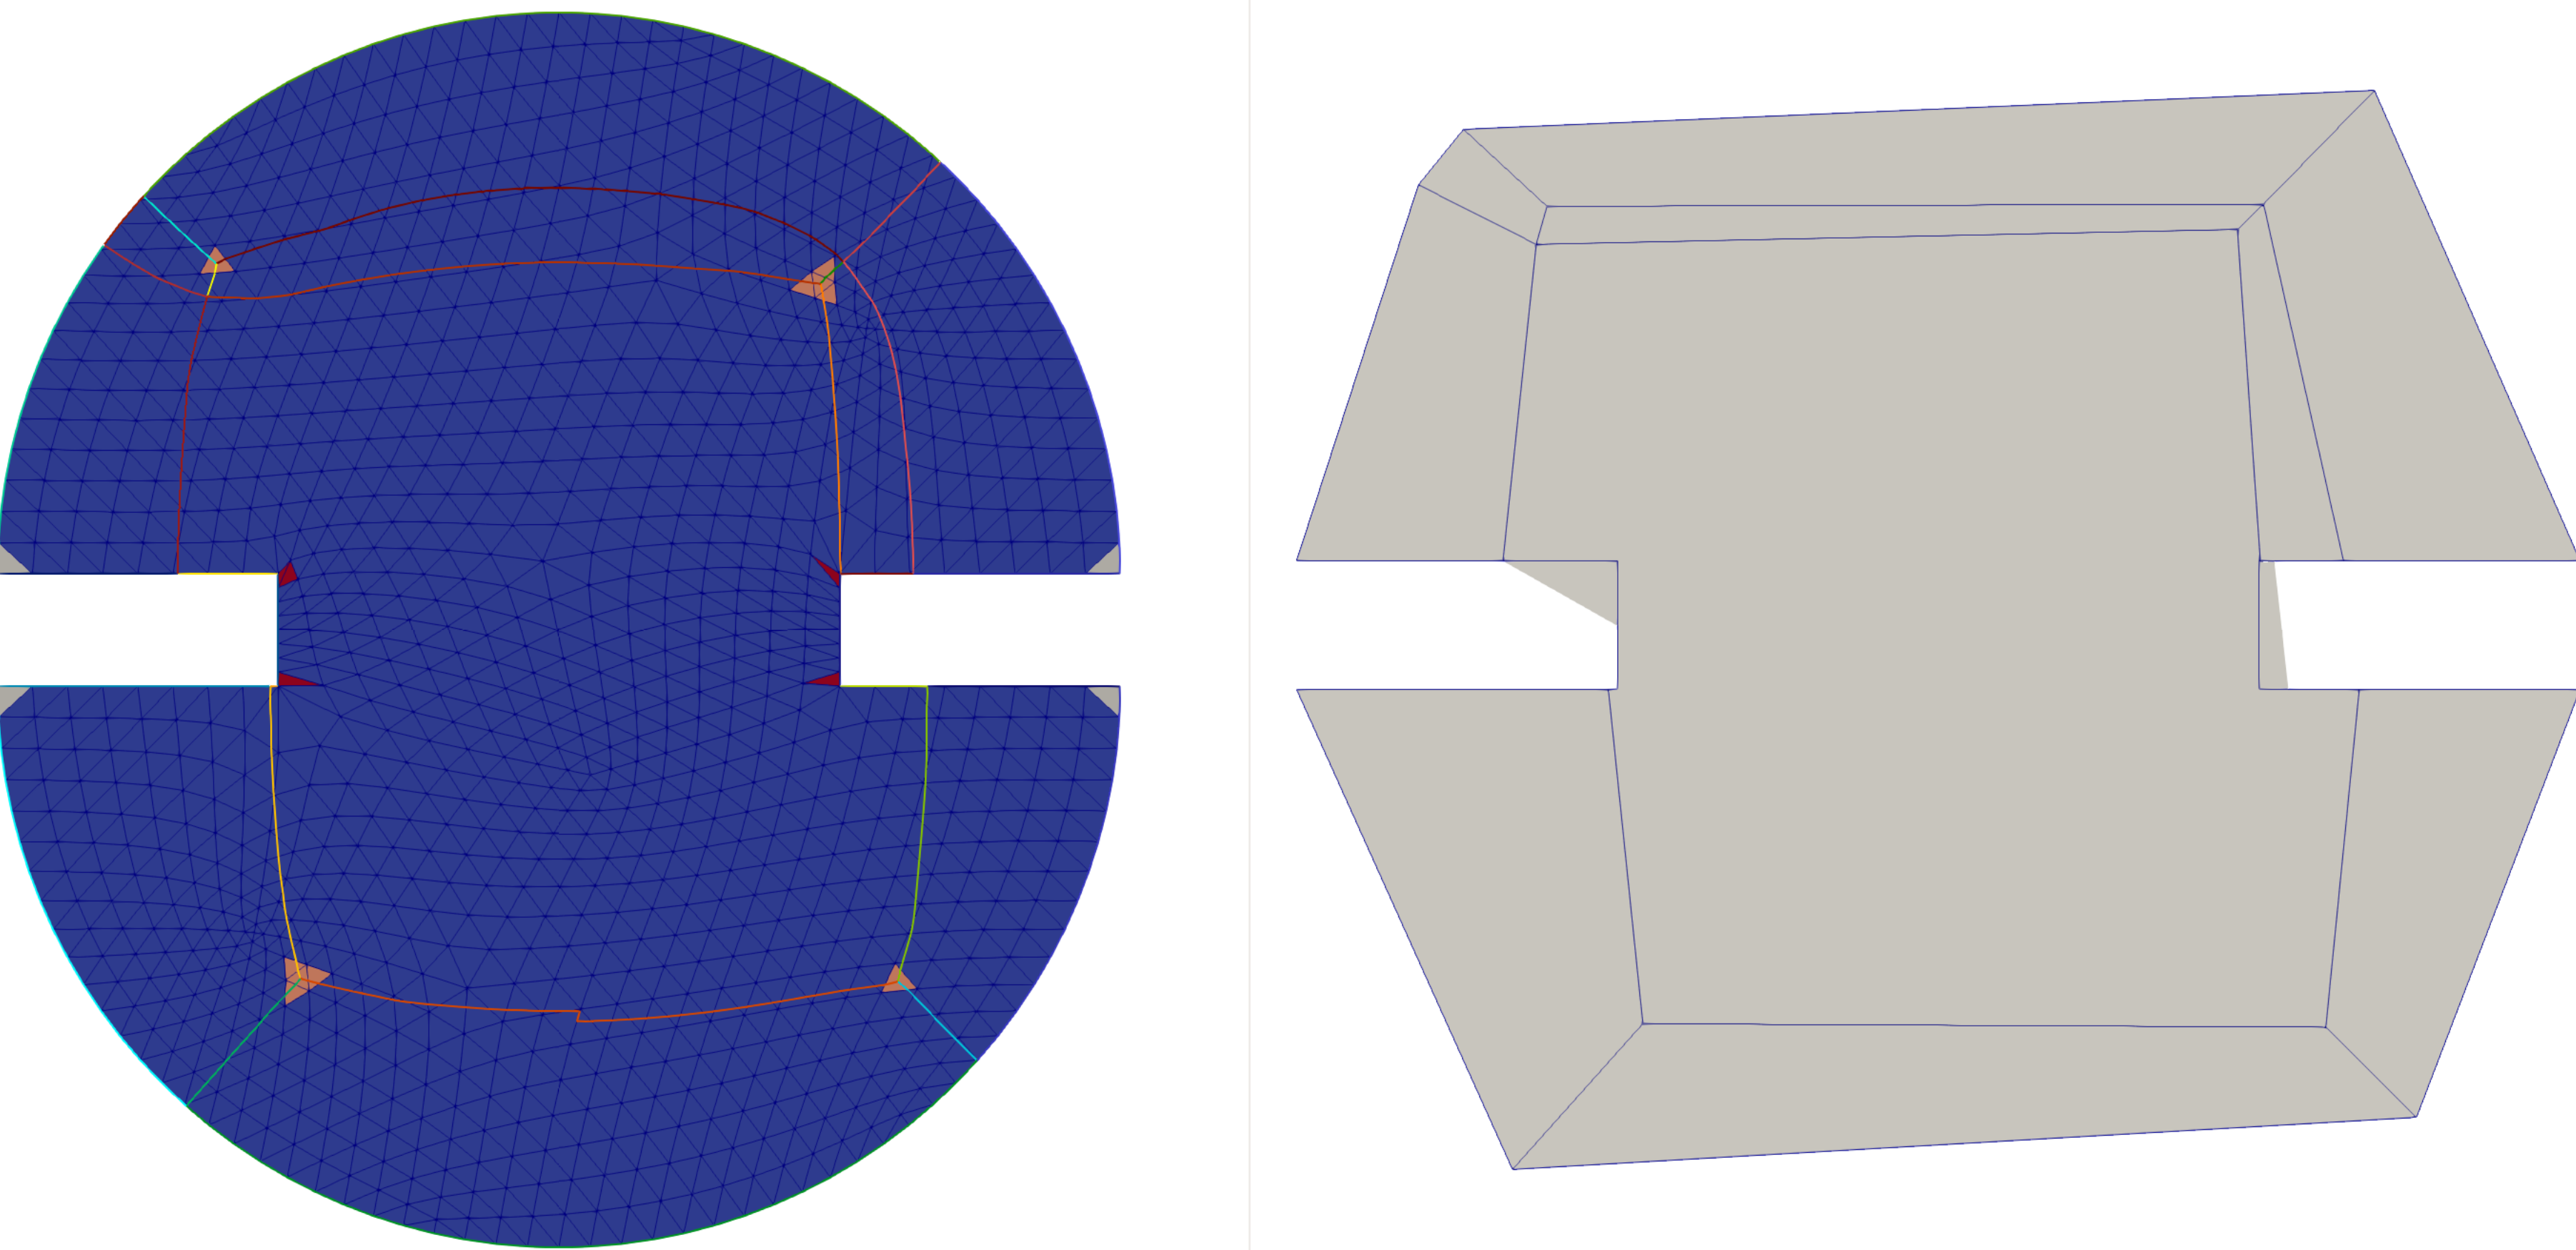
\includegraphics[width=10cm]
        {img/Circle_with_concavities_refSS1.png}}
        \caption{ Mesh Circle\_with\_concavities\_ref - SS1}
      \end{figure}
      }
      
      \frame{
      \begin{figure}[]
        \center{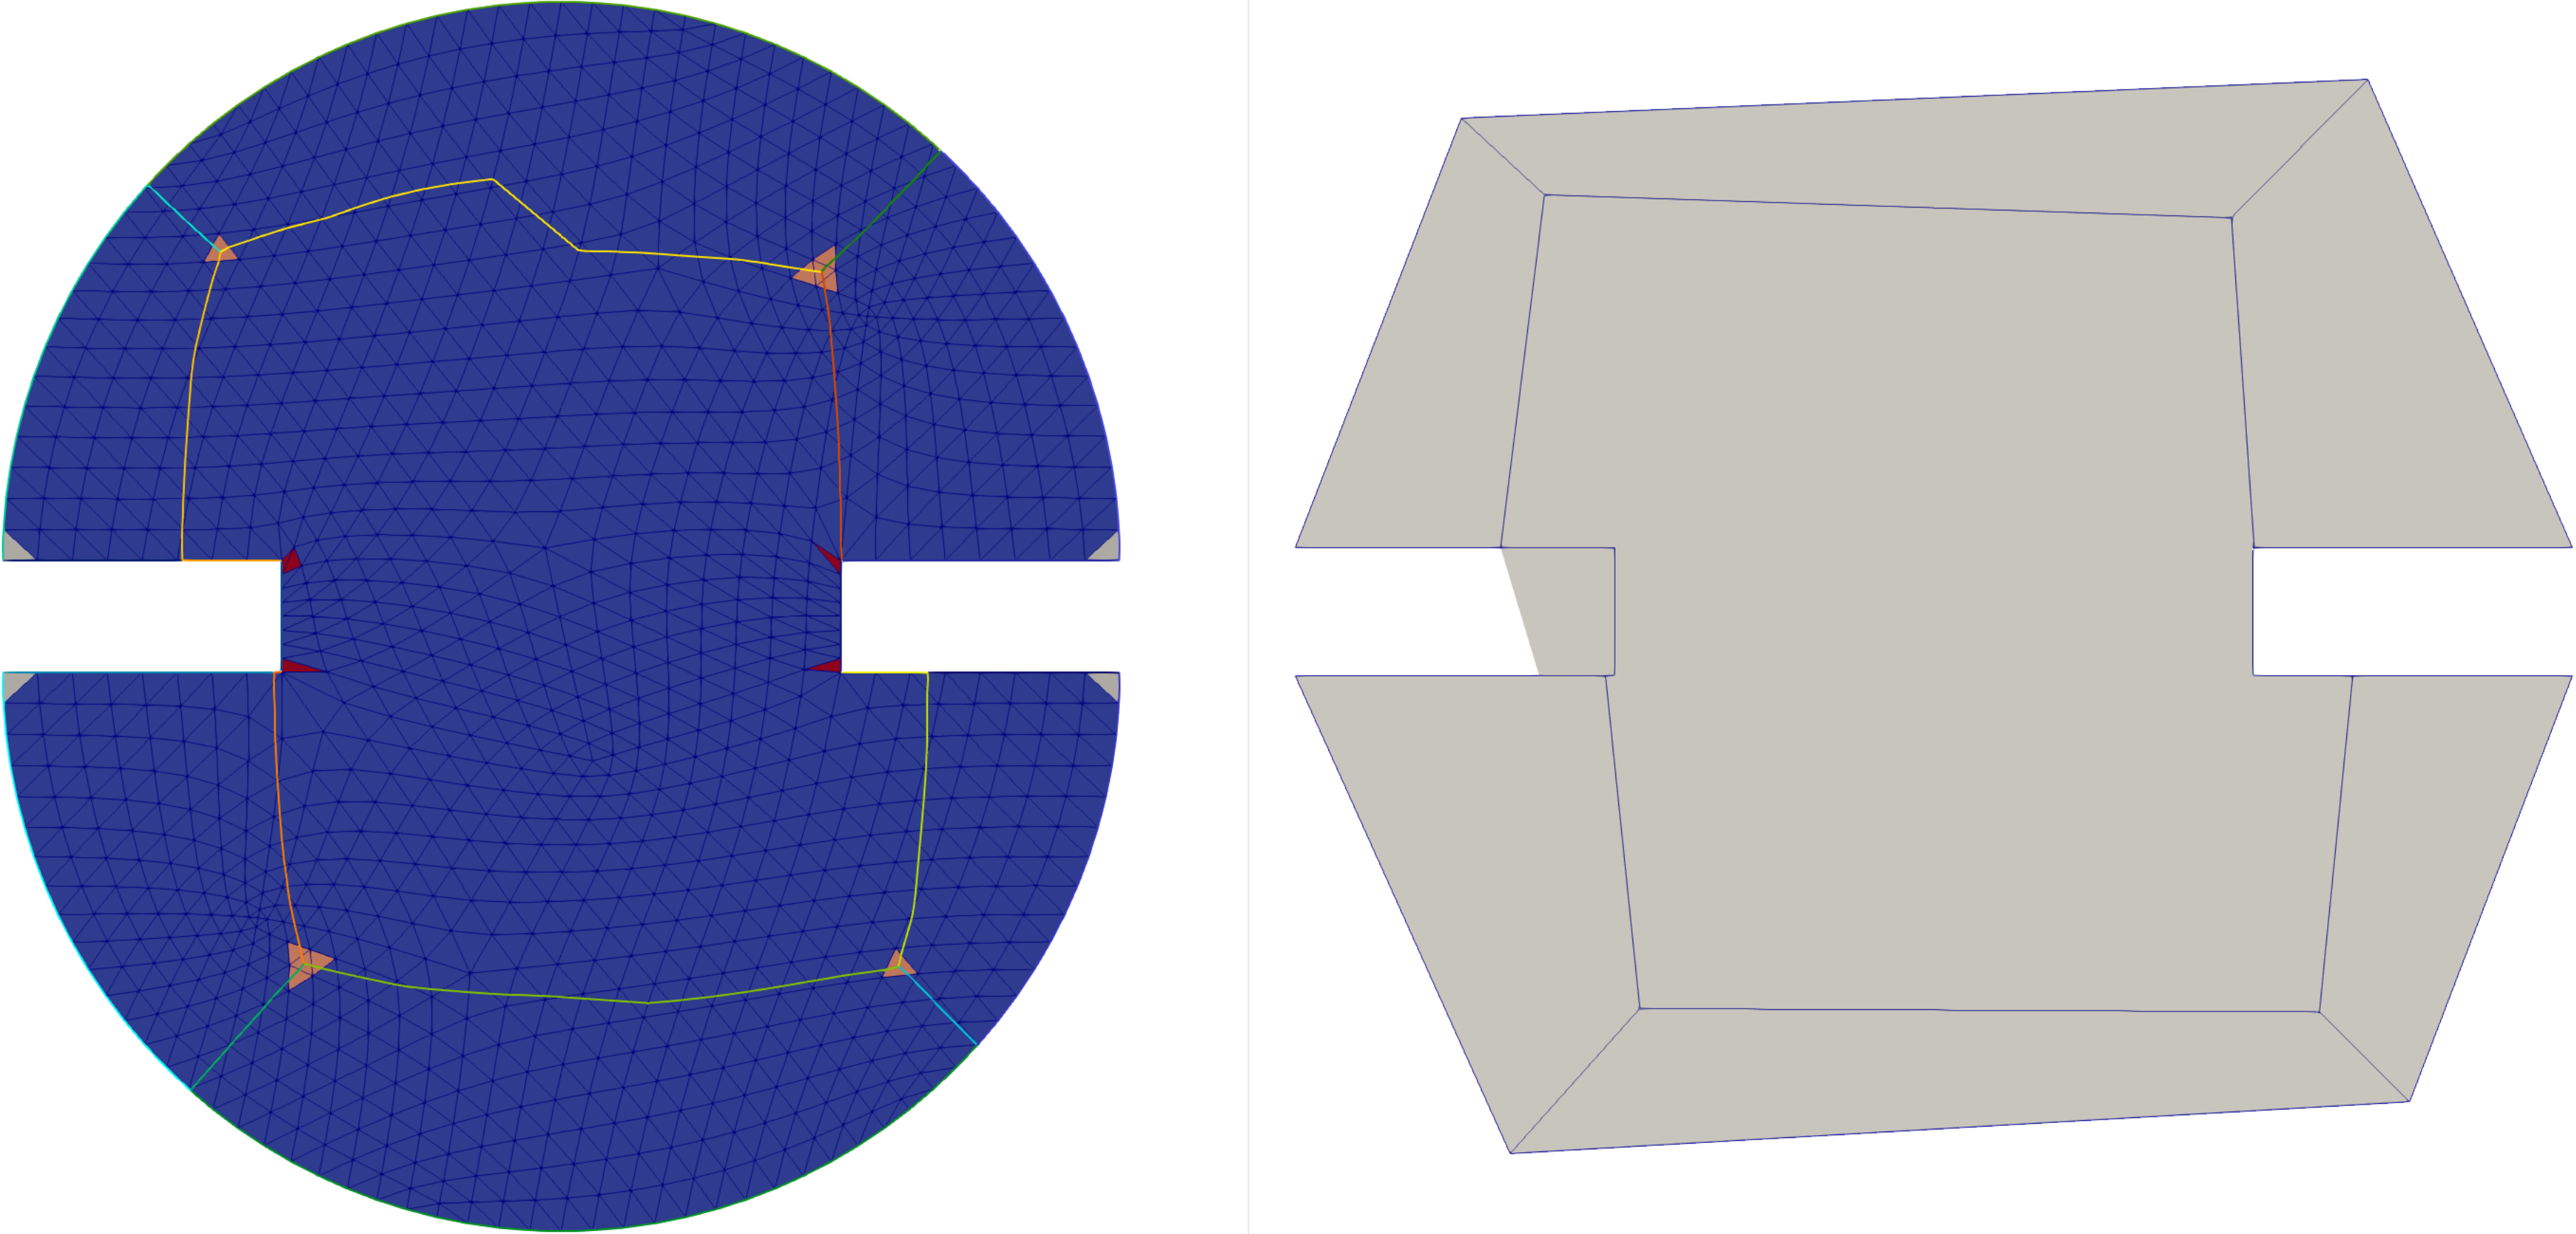
\includegraphics[width=10cm]
        {img/Circle_with_concavities_refSS4.png}}
        \caption{ Mesh Circle\_with\_concavities\_ref - SS4}
      \end{figure}
      }
      
%\frame{      
 %     \begin{figure}[]
 %      \center{\includegraphics[width=10cm]
 %     {img/Curved_Shape1SS5.png}}
 %    \caption{ Mesh Curved\_Shape1 - SS5}
 % \end{figure}
 %}   
    
    \frame{  
      \begin{figure}[]
        \center{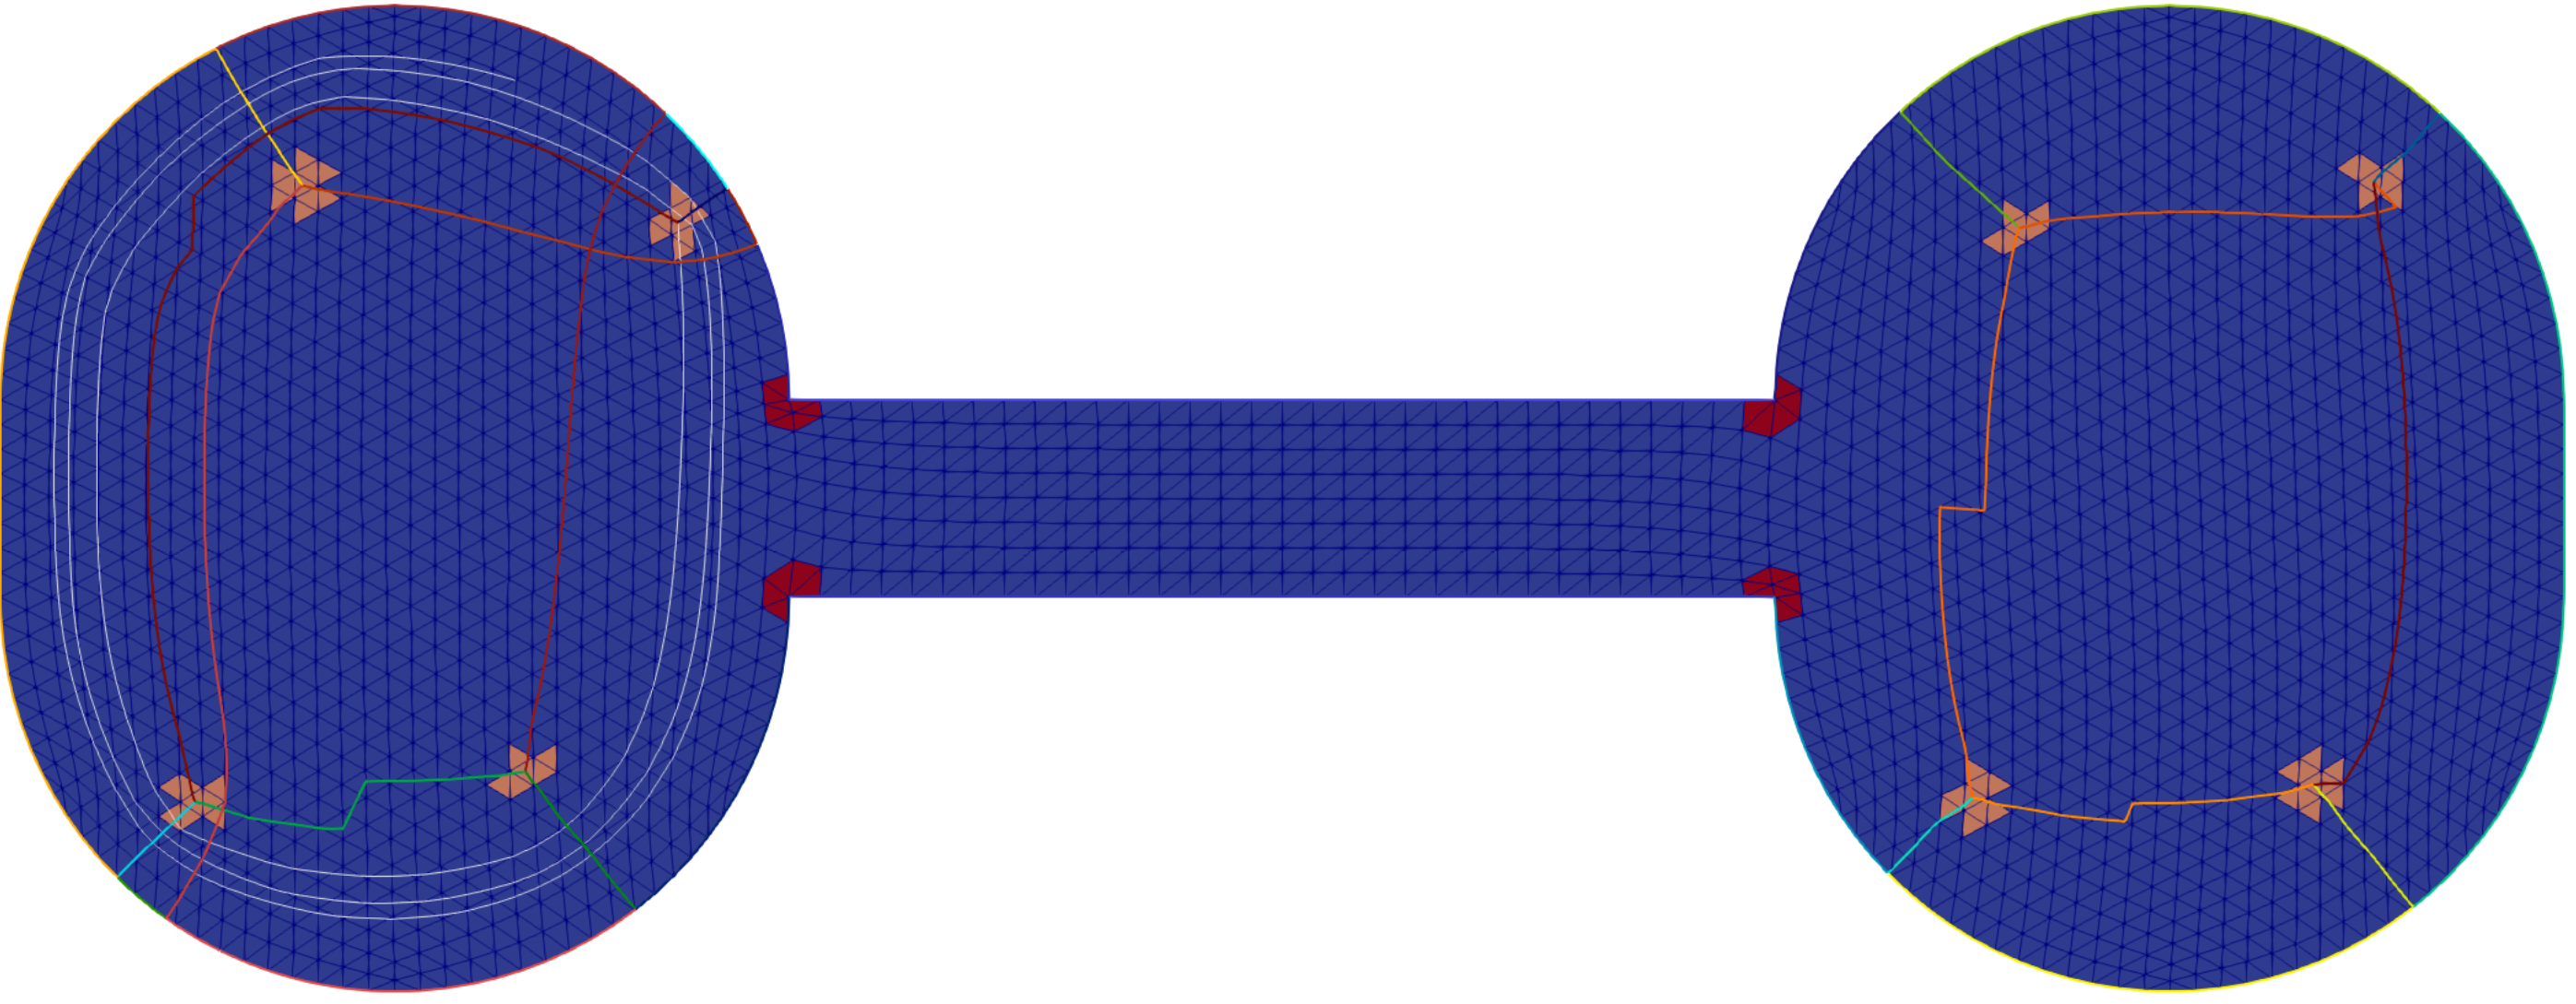
\includegraphics[width=10cm]
        {img/shape1SS2-cycle.png}}
        \caption{ Mesh shape1 - SS2}
      \end{figure}
      }
      
      
      \frame{
      \begin{figure}[]
        \center{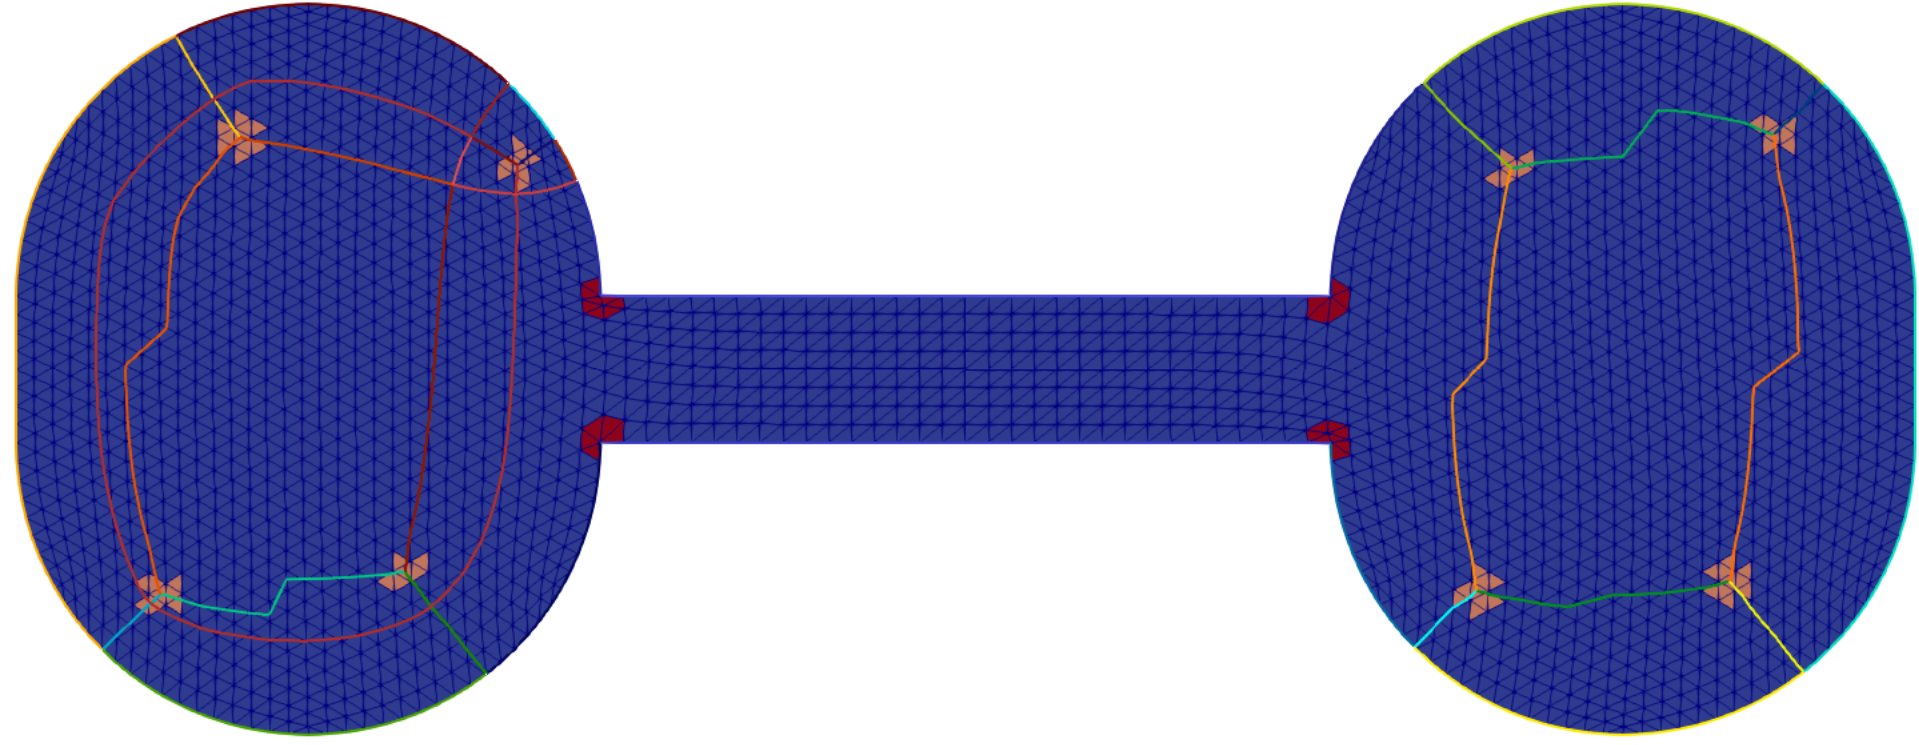
\includegraphics[width=10cm]
        {img/shape1SS3.png}}
        \caption{ Mesh shape1 - SS3}
      \end{figure}
}
	
\end{document}